\chapter{Konzeption}\label{chap:conception}
    \section{Gesamtarchitektur des Systems}\label{sec:overall-system-architecture}
        % müsste eigentlich Additiven Fertigung heißen wie geht das in latex?
        Das in dieser Arbeit entwickelte System verfolgt das Ziel, eine durchgängige Verarbeitungskette von der dreidimensionalen Bauteilgeometrie bis zur robotergestützten \gls{additive-manufacturing} bereitzustellen.
        Die Gesamtarchitektur gliedert sich in zwei eigenständige Softwarekomponenten: \ac{medusa} für die geometrische Planung und \ac{kronos} für die roboterkinematische Ausführung.
        Die folgenden Unterabschnitte beschreiben zunächst die leitenden Entwurfsprinzipien und anschließend den modularen Aufbau sowie die Begründung der gewählten Komponentenaufteilung.
        Abschließend wird die Schnittstelle beschrieben, über die beide Komponenten miteinander kommunizieren.
        \sig{Adrian Gabriel Axtmann}

        \subsection{Architekturprinzipien und Entwurfsziele}\label{subsec:architecture-principles-and-design-goals}
            Der Entwurf des Gesamtsystems orientiert sich an vier leitenden
            Architekturprinzipien.
            Die konkrete Umsetzung dieser Prinzipien in Form der Aufteilung in die Komponenten \ac{medusa} und \ac{kronos} wird in \cref{subsec:concept-component-separation-medusa-kronos} begründet.
            \sig{Adrian Gabriel Axtmann}

            \paragraph{Modularität}
                Das System wird in klar abgegrenzte Module mit definierten Schnittstellen unterteilt.
                Jedes Modul kapselt eine fachliche Verantwortlichkeit und ist unabhängig von der internen Realisierung anderer Module nutzbar.
                Dieses Prinzip ermöglicht den Austausch einzelner Komponenten, ohne die Gesamtarchitektur zu verändern.
                \sig{Adrian Gabriel Axtmann}

            \paragraph{Erweiterbarkeit}
                Neue \gls{slicing}-Algorithmen sollen integrierbar sein, ohne die nachgelagerten Verarbeitungsstufen oder die Roboteranbindung zu verändern.
                Ebenso soll die Anbindung alternativer Robotersysteme möglich sein, ohne die geometrische Planungskomponente anzupassen.
                Dieses Ziel wird durch eine wohldefinierte Schnittstelle zwischen den Komponenten sowie durch abstrakte Interfaces innerhalb der algorithmischen Schicht adressiert.
                \sig{Adrian Gabriel Axtmann}

            \paragraph{Plattformunabhängigkeit der Planungskomponente}
                Die Komponente \ac{medusa} wird so konzipiert, dass sie auf den Betriebssystemen Linux, macOS und Windows kompilier- und ausführbar ist.
                Plattformspezifische Anpassungen beschränken sich auf die Build-Konfiguration und die grafische Ausgabe.
                Die algorithmischen Kernfunktionen sind frei von plattformspezifischen Abhängigkeiten.
                \sig{Adrian Gabriel Axtmann}

            \paragraph{Unabhängigkeit der Lebenszyklen}
                Die beiden Komponenten sollen unabhängig voneinander entwickelt, getestet und in Betrieb genommen werden können.
                Insbesondere darf die algorithmische Entwicklung nicht an die Verfügbarkeit eines physischen Robotersystems gebunden sein.
                Umgekehrt muss die Inbetriebnahme der Robotersteuerung von einem bestimmten Stand der \gls{slicing}-Implementierung unabhängig sein.
                \sig{Adrian Gabriel Axtmann}

        \subsection{Modularer Aufbau und Verantwortlichkeiten}\label{subsec:modular-structure-and-responsibilities}
            Aus den genannten Prinzipien aus \cref{subsec:architecture-principles-and-design-goals} ergibt sich eine Zweiteilung des Gesamtsystems entlang der Grenze zwischen geometrischer Planung und roboterkinematischer Ausführung.
            \cref{tab:concept-component-responsibilities} fasst die Verantwortlichkeiten der beiden Komponenten zusammen.
            Die ausführliche fachliche Beschreibung erfolgt in \cref{sec:concept-of-software-components}.
            \sig{Adrian Gabriel Axtmann}

            \begin{figure}[ht]
                \centering
                \resizebox{\linewidth}{!}{
                        \begin{tikzpicture}[
    >=Latex,
    every node/.style={font=\small},
    component/.style={
        rectangle, rounded corners=6pt, draw, very thick,
        minimum width=4.6cm,
        minimum height=5.6cm,
        align=center, inner sep=8pt,
    },
    medusa/.style={component, fill=blue!6,  draw=blue!55!black},
    kronos/.style={component, fill=orange!8, draw=orange!60!black},
    submodule/.style={
        rectangle, rounded corners=2pt, draw, thin,
        fill=white, minimum width=3.8cm,
        minimum height=0.55cm,
        align=center, font=\scriptsize, inner sep=2pt,
    },
    domaintext/.style={
        font=\scriptsize\itshape, gray!60!black, align=center,
    },
    flow/.style={->, very thick, blue!50!black},
    iflow/.style={->, very thick, orange!60!black},
    iolabel/.style={font=\scriptsize\bfseries, gray!70!black,
                    align=center},
    extbox/.style={
        rectangle, rounded corners=2pt, draw, thin,
        fill=gray!10, minimum width=2.0cm, minimum height=1.0cm,
        align=center, font=\scriptsize,
    },
    inlinelbl/.style={
        font=\scriptsize, gray!70!black, align=center,
        fill=white, inner xsep=3pt, inner ysep=1pt,
    },
]
    % =========================================================
    % MEDUSA-Komponente (links)
    % =========================================================
    \node[medusa] (medusa) {};
    \node[font=\bfseries, anchor=north]
        at ([yshift=-4pt]medusa.north) {MEDUSA};
    \node[domaintext, anchor=north]
        at ([yshift=-22pt]medusa.north) {Domäne: Geometrie};

    \node[submodule, anchor=north]
        at ([yshift=-44pt]medusa.north) (m1) {Mesh-Import};
    \node[submodule, below=2pt of m1] (m2) {Geometrieaufbereitung};
    \node[submodule, below=2pt of m2] (m3) {Slicing-Algorithmen};
    \node[submodule, below=2pt of m3] (m4) {Toolpath-Planung};
    \node[submodule, below=2pt of m4] (m5) {3D-Viewer (OpenGL)};
    \node[submodule, below=2pt of m5] (m6) {JSON-Export};

    % =========================================================
    % KRONOS-Komponente (rechts)
    % =========================================================
    \node[kronos, right=3.0cm of medusa] (kronos) {};
    \node[font=\bfseries, anchor=north]
        at ([yshift=-4pt]kronos.north) {KRONOS};
    \node[domaintext, anchor=north]
        at ([yshift=-22pt]kronos.north) {Domäne: Roboterkinematik};

    \node[submodule, anchor=north]
        at ([yshift=-44pt]kronos.north) (k1) {JSON-Parser};
    \node[submodule, below=2pt of k1] (k2) {Planning Scene / Kollision};
    \node[submodule, below=2pt of k2] (k3) {Inverse Kinematik (TRAC-IK)};
    \node[submodule, below=2pt of k3] (k4) {Singularitätsbehandlung};
    \node[submodule, below=2pt of k4] (k5) {Postprozessor};
    \node[submodule, below=2pt of k5] (k6) {ROS\,2 / MoveIt-Anbindung};

% =========================================================
    % Schnittstelle: toolpath.json (datei-artig, etwas größer)
    % =========================================================
    \coordinate (mid) at ($(medusa.east)!0.5!(kronos.west)$);

    \begin{scope}[shift={(mid)}]
        \def\fw{0.75}   % halbe Breite  -> Gesamtbreite 1.5 cm
        \def\fh{0.55}   % halbe Höhe    -> Gesamthöhe   1.1 cm
        \def\fc{0.22}   % Eckenfase (rechts oben)
        % Korpus
        \fill[red!8]
            (-\fw,-\fh) -- (\fw,-\fh) -- (\fw,\fh-\fc)
            -- (\fw-\fc,\fh) -- (-\fw,\fh) -- cycle;
        \draw[red!55!black, thick]
            (-\fw,-\fh) -- (\fw,-\fh) -- (\fw,\fh-\fc)
            -- (\fw-\fc,\fh) -- (-\fw,\fh) -- cycle;
        % Knick-Linien (Faltkante)
        \draw[red!55!black, thick]
            (\fw-\fc,\fh) -- (\fw-\fc,\fh-\fc) -- (\fw,\fh-\fc);
        % Beschriftung
        \node[font=\scriptsize\ttfamily, align=center, text=red!35!black]
            at (0,-0.02) {toolpath\\.json};
        % Ankerpunkte für die Pfeile
        \coordinate (artwest)  at (-\fw,0);
        \coordinate (arteast)  at ( \fw,0);
        \coordinate (artnorth) at (0, \fh);
    \end{scope}

    \draw[flow]  (medusa.east) -- (artwest);
    \draw[iflow] (arteast)     -- (kronos.west);

    \node[inlinelbl, anchor=south]
        at ([yshift=6pt]artnorth)
        {dateibasiert,\\asynchron};

    % =========================================================
    % Eingabe (3D-Mesh)
    % =========================================================
    \node[extbox, left=1.2cm of medusa] (input) {3D-Datei\\(STL / OBJ)};
    \draw[flow] (input.east) -- (medusa.west);

    % =========================================================
    % Ausgabe (UR3e-Roboter) – etwas mehr Abstand für das Label
    % =========================================================
    \node[extbox, right=1.7cm of kronos] (robot) {UR3e\\(simuliert)};
    \draw[iflow] (kronos.east) -- (robot.west);

    \node[inlinelbl, anchor=south]
        at ([yshift=6pt]$(kronos.east)!0.5!(robot.west)$)
        {Joint-\\Trajektorien};

\end{tikzpicture}
                    }
                \caption[Gesamtarchitektur des Systems]{%
                    Gesamtarchitektur mit \ac{medusa} (Slicing) und \ac{kronos} (Robotersteuerung).
                    Die Kopplung erfolgt ausschließlich über das Dateiartefakt \texttt{toolpath.json}.
                }
                \label{fig:concept-system-architecture}
            \end{figure}

            \begin{table}[ht]
                \centering
                \caption[Verantwortlichkeiten der Systemkomponenten]
                        {Verantwortlichkeiten der Systemkomponenten und Aufzählung in Reihenfolge der Verarbeitungspipeline}
                \label{tab:concept-component-responsibilities}
                \begin{tabular}{@{} l l p{8.0cm} @{}}
                    \toprule
                    \textbf{Komponente} & \textbf{Domäne} & \textbf{Verantwortlichkeit} \\
                    \midrule
                    \ac{medusa} & Geometrie &
                        \begin{itemize}[leftmargin=*, nosep, label=--]
                            \item \gls{mesh}-Import
                            \item \gls{slicing}
                            \item \gls{infill}-Generierung
                            \item \gls{toolpath}-Planung
                            \item Echtzeit-Visualisierung
                        \end{itemize} \\
                    \addlinespace
                    \ac{kronos} & Roboterkinematik &
                        \begin{itemize}[leftmargin=*, nosep, label=--]
                            \item Entgegennahme des \gls{toolpath}
                            \item Transformation in 6-\ac{DOF}-Posen
                            \item \gls{inverse-kinematics}
                            \item \gls{singularity}-Behandlung
                            \item Kollisionsprüfung
                            \item \gls{postprocessor}
                            \item Ansteuerung des UR3e
                        \end{itemize} \\
                    \bottomrule
                \end{tabular}
            \end{table}

        \subsection{Komponentenabgrenzung MEDUSA und KRONOS}\label{subsec:concept-component-separation-medusa-kronos}
            Die in \cref{subsec:modular-structure-and-responsibilities} dargestellte Aufteilung in zwei eigenständige Komponenten ist keine reine Implementierungsentscheidung, sondern folgt aus vier sachlichen Gründen.

            \paragraph{Unterschiedliche fachliche Domänen}
                \ac{medusa} operiert im Bereich der algorithmischen Geometrieverarbeitung und Computergrafik, \ac{kronos} dagegen in der Domäne der Roboterkinematik und Steuerungstechnik.
                Eine Trennung entlang dieser Domänengrenze reduziert die Kopplung zwischen den Teilsystemen und erlaubt es, fachspezifische Bibliotheken und Programmiermodelle isoliert einzusetzen.
                \sig{Adrian Gabriel Axtmann}

            \paragraph{Unterschiedliche Laufzeitanforderungen}
                Die geometrische Planung in \ac{medusa} erfolgt als Offline-Prozess und unterliegt keinen Echtzeitbedingungen.
                Da die Berechnungsdauer komplexer Slicing-Algorithmen je nach Geometrie stark schwanken kann, ist ein nicht-deterministisches Zeitverhalten hier akzeptabel.
                Die roboterseitige Ausführung in \ac{kronos} ist hingegen an strikte, deterministische Kommunikationszyklen und an die aktive Sicherheitsüberwachung der Robotersteuerung gebunden.
                Industrieroboter wie der UR3e verlangen eine Ansteuerung in exakten Zeitintervallen (Echtzeit), um eine flüssige Trajektorienführung zu garantieren und Sicherheitsstopps zu vermeiden.
                Da Software-Frameworks wie \ac{ros} oder MoveIt inhärent nicht-deterministisch operieren, würden Rechenzeitschwankungen (Jitter) bei einer direkten Kopplung zum Abbruch der Kommunikation mit der Hardware führen.
                Diese gegensätzlichen Anforderungen werden durch die physische Trennung der Prozesse und ein explizites, asynchrones Übergabeformat aufgelöst, welches die geplanten Pfade von der zeitkritischen Ausführung entkoppelt.
                \sig{Adrian Gabriel Axtmann}

            \paragraph{Wiederverwendbarkeit der Planungskomponente}
                Die \gls{slicing}-Algorithmen und die \gls{toolpath}-Planung sind unabhängig vom konkreten Robotersystem.
                \ac{medusa} kann daher als Planungskomponente für unterschiedliche Roboter-Backends eingesetzt werden, sofern in der jeweiligen Ausführungskomponente ein kompatibler \gls{postprocessor} bereitgestellt wird.
                \sig{Adrian Gabriel Axtmann}

            \paragraph{Entkoppelte Entwicklungs- und Releasezyklen}
                Die Trennung der beiden Komponenten ermöglicht eine unabhängige Entwicklung sowie Test- und Validierungsprozesse.
                Die algorithmische Arbeit an \ac{medusa} ist nicht an die Verfügbarkeit des UR3e-Systems gebunden.
                In gleicher Weise kann \ac{kronos} unabhängig vom aktuellen Stand der \gls{slicing}-Algorithmen weiterentwickelt werden, sofern das vereinbarte Übergabeformat eingehalten wird.
                \sig{Adrian Gabriel Axtmann}

        \subsection{Datenflüsse und Schnittstellen zwischen den Modulen}\label{subsec:data-flows-and-interfaces-between-modules}
            Die zentrale Systemschnittstelle verläuft zwischen \ac{medusa} und \ac{kronos}.
            Sie besteht aus exakt einem Datenartefakt, dem von \ac{medusa} erzeugten \gls{toolpath}.
            Dieser bildet die vollständige Beschreibung des geplanten Fertigungspfads ab und ist die einzige Information, die zwischen den beiden Komponenten ausgetauscht wird.
            \sig{Adrian Gabriel Axtmann}

            \subsubsection{Anforderungen an die Schnittstelle}\label{subsubsec:interface-requirements}
                Die Anforderungen definieren den äußeren Rahmen der Schnittstelle, treffen jedoch keine Aussagen über die inhaltlichen Eigenschaften des Übergabeartefakts selbst.
                Aus ihnen lassen sich vier Eigenschaften ableiten:

                \begin{description}
                    \item[Vollständigkeit]
                        Damit \ac{kronos} ohne Zugriff auf interne Datenstrukturen von \ac{medusa} arbeiten kann, müssen pro Wegpunkt sowohl die geometrische Lage als auch alle prozessrelevanten Größen im Datenstrom enthalten sein.
                    \item[Selbstbeschreibung]
                        Aus Persistenz und Asynchronität folgt, dass kein gemeinsamer Laufzeitkontext existiert.
                        Das Artefakt muss daher Bezugssystem, Einheiten und erzeugenden \gls{slicing}-Algorithmus explizit mitführen.
                    \item[Versionierbarkeit]
                        Da \ac{medusa} und \ac{kronos} unabhängig voneinander entwickelt werden können, muss die Schnittstelle versionsbehaftet sein, sodass \ac{kronos} bei der Übernahme die Kompatibilität prüfen kann.
                \end{description}
                \sig{Adrian Gabriel Axtmann}

            \subsubsection{Aufbau des Toolpath-Artefakts}\label{subsubsec:interface-conceptual-structure}
                Der \gls{toolpath} ist zweischichtig aufgebaut.
                Ein \emph{Job-Header} beschreibt den gesamten Fertigungsauftrag, ein \emph{Wegpunktstrom} die geometrische und prozessuale Bewegungsfolge.
                Die Trennung erlaubt es, den Header einmalig vor Beginn der Ausführung zu validieren und den Wegpunktstrom anschließend sequenziell zu verarbeiten.
                \cref{tab:interface-header-fields} und \cref{tab:interface-waypoint-fields} fassen die jeweils enthaltenen Felder zusammen.

                \begin{table}[ht]
                    \centering
                    \caption[Felder des Job-Headers]{Felder des Job-Headers}
                    \label{tab:interface-header-fields}
                    \begin{tabular}{@{} l l p{6.5cm} @{}}
                        \toprule
                        \textbf{Feld} & \textbf{Typ} & \textbf{Bedeutung} \\
                        \midrule
                        Schemaversion       & SemVer-String   & Versionskennung der Schnittstellenspezifikation; Grundlage der Kompatibilitätsprüfung \\
                        Slicer-Version      & SemVer-String   & Versionskennung der erzeugenden \ac{medusa}-Instanz; Diagnose- und Reproduktionszweck \\
                        Algorithmus         & Aufzählung      & Bezeichner des verwendeten \gls{slicing}-Algorithmus (\emph{planar}, \emph{Base}, \emph{Kristall}) \\
                        Einheiten           & String-Tupel    & Festlegung der Einheiten für Position (\si{mm}) und Zeit (\si{s}) \\
                        Bezugssystem        & String          & Name des Koordinatensystems, in \ac{kronos} als TF-Frame interpretierbar \\
                        Erzeugungszeitpunkt & ISO-8601-String & Zeitstempel der Erzeugung; dient der Nachverfolgbarkeit \\
                        Wegpunkt-Prüfsumme  & 64-Bit Hex      & Nicht-kryptografische Prüfsumme über den serialisierten Wegpunktstrom \\
                        \bottomrule
                    \end{tabular}
                \end{table}

                \begin{table}[ht]
                    \centering
                    \caption[Felder eines Wegpunkts]{Felder eines Wegpunkts}
                    \label{tab:interface-waypoint-fields}
                    \begin{tabular}{@{} l l p{6.0cm} @{}}
                        \toprule
                        \textbf{Feld} & \textbf{Typ} & \textbf{Bedeutung} \\
                        \midrule
                        Position $(x, y, z)$                 & $\mathbb{R}^3$ in \si{mm}            & Lage der Werkzeugspitze \\
                        Orientierung $(q_w, q_x, q_y, q_z)$  & Einheits-\gls{quaternion}            & Werkzeugorientierung; ROS-/MoveIt-kompatibel \\
                        Vorschub                             & $\mathbb{R}_{\geq 0}$ in \si{mm/s}   & Bahngeschwindigkeit \\
                        Extrusionsrate                       & $\mathbb{R}_{\geq 0}$ in \si{mm^3/s} & Materialfluss; bei Verbindungswegen $0$ \\
                        Bewegungsart                         & $\{\text{print}, \text{travel}\}$    & Steuert Geschwindigkeitsprofil \\
                        Schichtindex                         & $\mathbb{N}_0$                       & Zugehörige Schicht; monoton nicht-fallend \\
                        Segmentindex                         & $\mathbb{N}_0$                       & Position innerhalb der Schicht; Diagnose und Wiederaufnahme \\
                        \Gls{branch}-Bezeichner              & $\mathbb{N}_0$, optional             & Identifiziert die \gls{branch} bei Base und Kristall \\
                        \bottomrule
                    \end{tabular}
                \end{table}

                Es wurde bewusst eine \emph{wegpunkt-} und keine \emph{segmentbasierte} Repräsentation gewählt.
                Ein Segment ergibt sich implizit aus zwei aufeinanderfolgenden Wegpunkten, ohne redundante Endpunkte zu übertragen.
                Die Quaternionen-Repräsentation der Orientierung vermeidet den Gimbal-Lock-Effekt von Eulerwinkeln, ist kompakter als eine Rotationsmatrix und korrespondiert unmittelbar mit der ROS-2-/MoveIt-Posendarstellung in \ac{kronos}.
                \sig{Adrian Gabriel Axtmann}

            \subsubsection{Übergabemechanismus}\label{subsubsec:interface-handover-mechanism}
                Aus der geforderten Persistenz, Asynchronität und manuellen Bedienbarkeit folgt unmittelbar ein dateibasierter Austausch.
                Ein \gls{ipc}-Mechanismus wie ROS-2-Topics würde einen gemeinsamen Lebenszyklus beider Prozesse erzwingen und widerspricht damit der geforderten Entkopplung.
                Als konkretes Dateiformat wurde \gls{json} gewählt, da es textbasiert und damit menschenlesbar, durch \gls{json-schema} formal spezifizierbar und sowohl in der \texttt{C++}-Welt von \ac{medusa} als auch in der ROS-2-Welt von \ac{kronos} nativ unterstützt wird.
                Binäre Alternativen wie, \texttt{Protocol Buffers}, sind speichereffizienter, stehen jedoch im Widerspruch zur Werkzeugunabhängigkeit und der manuellen Bedienbarkeit.
                \sig{Adrian Gabriel Axtmann}

    \section{Konzeption der Softwarekomponenten}\label{sec:concept-of-software-components}
        Die folgenden Unterabschnitte beschreiben die beiden Softwarekomponenten des Systems im Detail.
        Während \cref{sec:overall-system-architecture} die Aufteilung und das Zusammenspiel beider Komponenten auf Architekturebene begründet, wird hier die innere Konzeption jeder Komponente beschrieben.

        \subsection{Komponente MEDUSA}\label{subsec:component-medusa}
            Im Mittelpunkt der Konzeption von \ac{medusa} stehen die Verarbeitungspipeline, die Aufteilung in fachliche Module, die zentralen Datenrepräsentationen sowie die Konzepte für Visualisierung und Bedienung.
            \sig{Adrian Gabriel Axtmann}

            \subsubsection{Verarbeitungspipeline}\label{subsubsec:concept-medusa-pipeline} \index{MEDUSA!Pipeline}
                Die innere Verarbeitungskette von \ac{medusa} ist als gerichteter azyklischer Datenfluss vom geladenen \gls{mesh} bis zum exportierten \gls{toolpath} organisiert.
                Sie gliedert sich in fünf aufeinander aufbauende Stufen:

                \begin{enumerate}
                    \item \emph{Mesh-Import}: Einlesen einer 3D-Datei (z.\,B. STL oder OBJ) und Überführung in eine interne Geometriedatenstruktur
                    \item \emph{Geometrieaufbereitung}: Verschweißen identischer \glspl{vertex}, Berechnung von Adjazenz, \gls{vertex}-Normalen und der \ac{AABB} des Bauteils
                    \item \emph{Slicing}: Anwendung eines der in \cref{sec:concept-of-slicing-strategies} beschriebenen Verfahren auf die aufbereitete Geometrie
                    \item \emph{Toolpath-Aufbereitung}: Zusammenführung der Schichtdaten zu einer linearen Wegpunktfolge und Anreicherung mit Pose, Vorschub und Bewegungsart
                    \item \emph{Export}: Serialisierung des \glspl{toolpath} in das in \cref{subsubsec:interface-conceptual-structure} definierte \gls{json}-Schema und atomare Ablage im Übergabeverzeichnis
                \end{enumerate}

                \begin{figure}[ht]
                    \centering
                    \resizebox{\linewidth}{!}{
                        % =====================================================================
%  MEDUSA – Verarbeitungspipeline (einreihig, Labels über den Boxen)
%
%  Benötigte TikZ-Bibliotheken (im Hauptdokument):
%      \usetikzlibrary{arrows.meta, positioning, calc, fit, backgrounds}
% =====================================================================

\providecommand{\stagenum}[1]{{\footnotesize\bfseries\color{blue!55!black}#1}}
\providecommand{\stagettl}[1]{{\scriptsize\bfseries\shortstack[c]{#1}}}

\begin{tikzpicture}[
    >=Latex,
    node distance=0.5cm,
    every node/.style={font=\footnotesize},
    %
    stage/.style={
        rectangle, rounded corners=3pt,
        draw=blue!55!black, thick,
        top color=blue!4, bottom color=blue!14,
        minimum width=2.0cm, minimum height=2.0cm,
        align=center, inner sep=3pt,
    },
    flow/.style={->, line width=0.7pt, draw=blue!55!black},
    flowlabel/.style={
        font=\scriptsize, text=black!75,
        inner xsep=2pt, inner ysep=1pt, align=center,
    },
    iolabel/.style={font=\scriptsize\bfseries, text=black!75, align=center},
    viz/.style={
        rectangle, rounded corners=3pt,
        draw=green!45!black, thick, dashed,
        fill=green!6, inner sep=6pt, align=center,
    },
    vizflow/.style={->, dashed, line width=0.6pt, draw=green!45!black},
]
% --------------------------- Stufen ----------------------------------
\node[stage] (s1) {%
    \stagenum{1}\\[1pt]\stagettl{Schicht-\\positionen}\\[4pt]
    \begin{tikzpicture}[baseline]
        \draw[gray!55] (0,0) rectangle (0.55,0.4);
        \foreach \y in {0.08,0.20,0.32}
            \draw[blue!65!black, thin] (-0.04,\y) -- (0.59,\y);
    \end{tikzpicture}};

\node[stage, right=of s1] (s2) {%
    \stagenum{2}\\[1pt]\stagettl{Schnitt}\\[4pt]
    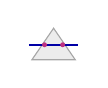
\begin{tikzpicture}[baseline]
        \fill[gray!15] (0,0)--(0.55,0)--(0.275,0.4)--cycle;
        \draw[gray!70] (0,0)--(0.55,0)--(0.275,0.4)--cycle;
        \draw[blue!65!black, thick] (-0.04,0.19)--(0.59,0.19);
        \fill[magenta!75!black] (0.16,0.19) circle (0.9pt);
        \fill[magenta!75!black] (0.39,0.19) circle (0.9pt);
    \end{tikzpicture}};

\node[stage, right=of s2] (s3) {%
    \stagenum{3}\\[1pt]\stagettl{Verkettung}\\[4pt]
    
\begin{tikzpicture}[baseline]
        \draw[magenta!75!black, very thick, rounded corners=1pt]
            (0.07,0.10)--(0.20,0.05)--(0.38,0.05)--
            (0.50,0.15)--(0.50,0.28)--(0.38,0.37)--
            (0.20,0.37)--(0.07,0.28)--cycle;
    \end{tikzpicture}};

\node[stage, right=of s3] (s4) {%
    \stagenum{4}\\[1pt]\stagettl{Reihenfolge}\\[4pt]
    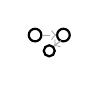
\begin{tikzpicture}[baseline]
        \draw[thick] (0.10,0.30) circle (0.08);
        \draw[thick] (0.46,0.30) circle (0.08);
        \draw[thick] (0.28,0.10) circle (0.07);
        \draw[->, thin, gray!70, dashed] (0.19,0.30)--(0.37,0.30);
        \draw[->, thin, gray!70, dashed] (0.43,0.23)--(0.34,0.16);
    \end{tikzpicture}};

\node[stage, right=of s4] (s5) {%
    \stagenum{5}\\[1pt]\stagettl{Emission}\\[4pt]
    
\begin{tikzpicture}[baseline]
        \draw[gray!70] (0.05,0) rectangle (0.52,0.4);
        \foreach \y in {0.08,0.16,0.24,0.32}
            \draw[gray!55, thin] (0.10,\y)--(0.47,\y);
    \end{tikzpicture}};

% --------------------------- Datenfluss-Pfeile -----------------------
\draw[flow] (s1.east) -- (s2.west);
\draw[flow] (s2.east) -- (s3.west);
\draw[flow] (s3.east) -- (s4.west);
\draw[flow] (s4.east) -- (s5.west);

% --------------------------- Labels ÜBER den Boxen -------------------
\node[flowlabel, above=2pt]
    at ($(s1.north east)!0.5!(s2.north west)$) {Höhen $a_i$};
\node[flowlabel, above=2pt]
    at ($(s2.north east)!0.5!(s3.north west)$) {Segmente};
\node[flowlabel, above=2pt]
    at ($(s3.north east)!0.5!(s4.north west)$) {Konturringe};
\node[flowlabel, above=2pt]
    at ($(s4.north east)!0.5!(s5.north west)$) {geordnete Ringe};

% --------------------------- I/O -------------------------------------
\draw[flow] ([xshift=-0.8cm]s1.west) -- (s1.west);
\node[iolabel, anchor=east] at ([xshift=-0.85cm]s1.west) {\gls{mesh}};

\draw[flow] (s5.east) -- ([xshift=0.8cm]s5.east);
\node[iolabel, anchor=west] at ([xshift=0.85cm]s5.east)
    {Schicht-\\datensatz};

% --------------------------- Viz-Box ---------------------------------
\node[viz,
      fit={(s1.south west) (s5.south east)},
      inner xsep=6pt, inner ysep=10pt,
      minimum height=1.1cm,
      yshift=-1.3cm] (vizfit)
    {\textbf{\footnotesize Visualisierung}~\scriptsize(3D-Viewer, OpenGL)\\[3pt]%
     \scriptsize\itshape read-only Zugriff auf jede Pipeline-Stufe};

\foreach \s in {s1,s2,s3,s4,s5}
    \draw[vizflow] (\s.south) -- (\s.south |- vizfit.north);

\end{tikzpicture}
                    }
                    \caption[Verarbeitungspipeline von MEDUSA]{
                        Verarbeitungspipeline von \ac{medusa} mit fünf Stufen und read-only Visualisierungs-Abzweigung.
                        Jede Stufe erzeugt eine isoliert testbare Zwischenrepräsentation.
                    }
                    \label{fig:concept-medusa-pipeline}
                \end{figure}

                Parallel zu dieser Hauptkette existiert eine \emph{Visualisierungs-Abzweigung}, die in jeder Stufe lesend auf den jeweils aktuellen Zwischenzustand zugreifen kann.
                Sie ist read-only, sodass die Darstellung im 3D-Viewer den eigentlichen Verarbeitungszustand nicht verändert und sich beliebig zu- oder abschalten lässt.
                Die strikte Stufung erlaubt es, jede Stufe isoliert zu testen und einzelne Stufen (insbesondere die Slicing-Stufe) unter Beibehaltung der übrigen Pipeline auszutauschen.
                \sig{Adrian Gabriel Axtmann}

            \subsubsection{Innere Modularisierung}\label{subsubsec:concept-medusa-modularization} \index{MEDUSA!Module}
                Die in \cref{subsec:architecture-principles-and-design-goals} formulierten Prinzipien der Modularität und Erweiterbarkeit werden innerhalb von \ac{medusa} durch eine Schichtenarchitektur umgesetzt.
                Jedes Modul kapselt eine fachliche Verantwortlichkeit und kennt ausschließlich die Schnittstellen darunterliegender Schichten.
                Insbesondere kennt kein Domänen- oder Infrastrukturmodul die Präsentationsschicht.
                Dadurch bleiben die algorithmischen Kernfunktionen frei von UI- und Renderingabhängigkeiten und sind eigenständig wiederverwendbar.

                \begin{figure}[ht]
                    \centering
                    \resizebox{\linewidth}{!}{
                        \begin{tikzpicture}[
    >=Latex,
    every node/.style={font=\small},
    layer/.style={
        rectangle, rounded corners=4pt, draw, very thick,
        minimum width=11.0cm, minimum height=1.4cm,
        align=center, inner sep=6pt,
    },
    composition/.style={layer, fill=purple!10, draw=purple!55!black},
    presentation/.style={layer, fill=blue!8,    draw=blue!55!black},
    interface/.style={layer, fill=red!8,        draw=red!55!black},
    domainlayer/.style={layer, fill=green!10,   draw=green!45!black},
    infrastructure/.style={layer, fill=gray!15, draw=gray!60!black},
    module/.style={
        rectangle, rounded corners=2pt, draw, thin,
        fill=white, minimum width=2.4cm, minimum height=0.65cm,
        align=center, font=\scriptsize\ttfamily, inner sep=2pt,
    },
    layerlabel/.style={
        font=\bfseries\small, anchor=west, inner sep=2pt,
    },
    dep/.style={->, very thick, blue!50!black},
    sidenote/.style={
        font=\scriptsize\itshape, gray!65!black,
        align=left, anchor=west,
    },
]
    % =========================================================
    % Schichten (von oben nach unten)
    % =========================================================
    \node[composition]                                  (L1) {};
    \node[presentation,    below=0.35cm of L1]          (L2) {};
    \node[interface,       below=0.35cm of L2]          (L3) {};
    \node[domainlayer,     below=0.35cm of L3]          (L4) {};
    \node[infrastructure,  below=0.35cm of L4]          (L5) {};

    % =========================================================
    % Schicht-Beschriftungen (links)
    % =========================================================
    \node[layerlabel, anchor=east]
        at ([xshift=-4pt]L1.west) {Komposition};
    \node[layerlabel, anchor=east]
        at ([xshift=-4pt]L2.west) {Präsentation};
    \node[layerlabel, anchor=east]
        at ([xshift=-4pt]L3.west) {Schnittstelle};
    \node[layerlabel, anchor=east]
        at ([xshift=-4pt]L4.west) {Domäne};
    \node[layerlabel, anchor=east]
        at ([xshift=-4pt]L5.west) {Infrastruktur};

    % =========================================================
    % Module pro Schicht
    % =========================================================
    % Komposition
    \node[module] at (L1) {app};

    % Präsentation: graphics, ui, controls
    \node[module] (m_graphics) at ([xshift=-3.0cm]L2.center) {graphics};
    \node[module] (m_ui)       at (L2.center)                {ui};
    \node[module] (m_controls) at ([xshift=3.0cm]L2.center)  {controls};

    % Schnittstelle: exporter
    \node[module] at (L3) {exporter};

    % Domäne: geometry, slicing
    \node[module] (m_geometry) at ([xshift=-1.6cm]L4.center) {geometry};
    \node[module] (m_slicing)  at ([xshift=1.6cm]L4.center)  {slicing};

    % Infrastruktur: core
    \node[module] at (L5) {core};

    % =========================================================
    % Abhängigkeitsrichtung (Pfeil rechts neben den Schichten)
    % =========================================================
    \draw[dep, very thick]
        ([xshift=0.6cm]L1.east) -- ([xshift=0.6cm]L5.east)
        node[midway, sloped, above, font=\scriptsize, gray!70!black]
        {Abhängigkeitsrichtung};

    % =========================================================
    % Erläuterungen rechts
    % =========================================================
    \node[sidenote] at ([xshift=1.3cm]L1.east)
        {kennt alle\\anderen Schichten};
    \node[sidenote] at ([xshift=1.3cm]L2.east)
        {Fenster, GUI,\\Eingabe};
    \node[sidenote] at ([xshift=1.3cm]L3.east)
        {JSON-Serialisierung};
    \node[sidenote] at ([xshift=1.3cm]L4.east)
        {Mesh, Slicing-\\Algorithmen};
    \node[sidenote] at ([xshift=1.3cm]L5.east)
        {Logging,\\Basisfunktionen};

\end{tikzpicture}
                    }
                    \caption[Schichtenarchitektur der MEDUSA-Module]{
                        Schichten\-architektur von \ac{medusa}.
                        Die Abhängigkeits\-richtung verläuft strikt von oben nach unten; nur die Kompositions\-schicht (\texttt{app}) verdrahtet alle Module.
                    }
                    \label{fig:concept-medusa-layered-architecture}
                \end{figure}

                \cref{tab:concept-medusa-modules} fasst die Verantwortlichkeit jedes Moduls zusammen.

                \begin{table}[ht]
                    \centering
                    \caption[Verantwortlichkeiten der MEDUSA-Module]{Verantwortlichkeiten der MEDUSA-Module, gruppiert nach Schichten der Modularchitektur}
                    \label{tab:concept-medusa-modules}
                    \begin{tabular}{@{} l l p{6.5cm} @{}}
                        \toprule
                        \textbf{Schicht} & \textbf{Modul} & \textbf{Verantwortlichkeit} \\
                        \midrule
                        Infrastruktur & \texttt{core}     & Strukturiertes asynchrones Logging über einen rotierenden Dateisink, gemeinsame Hilfstypen, plattformübergreifende Basisfunktionen \\
                        \midrule
                        \multirow{2}{*}{Domäne}
                                    & \texttt{geometry} & \gls{mesh}-Datenstrukturen, Adjazenz, \ac{AABB} \\
                                    & \texttt{slicing}  & Implementierung der Slicing-Strategien \\
                        \midrule
                        Schnittstelle & \texttt{exporter} & Validierung und Serialisierung des \glspl{toolpath} nach \gls{json} \\
                        \midrule
                        \multirow{3}{*}{Präsentation}
                                    & \texttt{graphics} & OpenGL-Renderer für \gls{mesh}, Schichten und \gls{toolpath} \\
                                    & \texttt{ui}       & ImGui-basierte Bedienoberfläche und Dockspace \\
                                    & \texttt{controls} & Eingabe- und Kamerabehandlung \\
                        \midrule
                        Komposition   & \texttt{app}      & Lebenszyklus, Fensterverwaltung, Verkettung der Module \\
                        \bottomrule
                    \end{tabular}
                \end{table}

                Die Trennung in eine Domänen- und eine Präsentationsschicht folgt einem bewussten Entwurfsprinzip.
                Sie erlaubt den Betrieb der algorithmischen Kernfunktionen in einem reinen Bibliotheksmodus ohne Fenster und OpenGL-Kontext, z.\,B. für automatisierte Tests in der \gls{ci-pipeline}.
                Darüber hinaus lässt sich die Präsentationsschicht austauschen, z.\,B. indem die ImGui-Oberfläche durch ein Kommandozeileninterface ersetzt wird, ohne dass die Slicing-Module davon berührt werden.
                Die Komposition aller Schichten zu einer lauffähigen Anwendung übernimmt das \texttt{app}-Modul, das als einziges Modul Kenntnis aller anderen besitzt.
                \sig{Adrian Gabriel Axtmann}

            \subsubsection{Zentrale Datenrepräsentationen}\label{subsubsec:concept-medusa-data-representations} \index{MEDUSA!Datenmodelle}
                Innerhalb der Pipeline zirkulieren drei klar abgegrenzte Datenrepräsentationen, welche die Schnittstellen zwischen den Stufen bilden.
                Jede Repräsentation ist nach ihrer Erzeugung als semi-immutabel zu behandeln.
                Nachgelagerte Stufen lesen ausschließlich, modifizieren jedoch nicht.

                \paragraph{Indizierte Dreiecksrepräsentation}
                    Die zentrale Geometriedatenstruktur ist eine indizierte Dreiecksrepräsentation, in der \glspl{vertex}, Normalen, Flächenindizes sowie vorab berechnete Adjazenz- und Inzidenzlisten gemeinsam abgelegt werden.
                    Die Vorabberechnung der Adjazenz erfolgt einmalig im Anschluss an den Import und vermeidet so wiederholte Suchoperationen in den nachgelagerten Slicing-Verfahren, welche intensiv auf Nachbarflächen-Beziehungen angewiesen sind.
                    Identische \glspl{vertex} aus dem Import werden über positionsbasiertes Verschmelzen zu gemeinsamen Indizes zusammengeführt.
                    Eine darüber hinausgehende Mesh-Reparatur findet nicht statt.
                    Die in \cref{subsubsec:concept-medusa-assumptions-limits} beschriebene Verantwortung für eine \gls{watertight} Eingabe verbleibt beim Benutzer.
                    \sig{Adrian Gabriel Axtmann}

                \paragraph{Schichtfolge}
                    Das Zwischenprodukt der Slicing-Stufe ist eine geordnete Folge von Schichten in der in \cref{subsubsec:concept-planar-layer-representation} festgelegten gemeinsamen Repräsentation.
                    Die einheitliche Schichtdarstellung über alle drei Slicing-Strategien hinweg ist entscheidend.
                    Dadurch kann die nachgelagerte Toolpath-Aufbereitung algorithmenagnostisch arbeiten und das System in \cref{sec:concept-of-slicing-strategies} um weitere Strategien erweitert werden, ohne den Exporter anzupassen.
                    \sig{Adrian Gabriel Axtmann}

                \paragraph{Toolpath}
                    Das Endprodukt der Pipeline ist der \gls{toolpath} in \cref{subsubsec:interface-conceptual-structure} spezifizierten Aufbau.
                    Die Konvertierung von der internen Schichtfolge in den exportierten \gls{toolpath} ist die einzige Stelle, an der Wegpunkte mit Vorschub, Extrusionsrate und Bewegungsart angereichert werden.
                    Vorher existieren diese prozessualen Größen ausschließlich als Parameter, nicht als Datenfeld.
                    \sig{Adrian Gabriel Axtmann}

            \subsubsection{Konzept der 3D-Visualisierung}\label{subsubsec:concept-medusa-visualization} \index{MEDUSA!Visualisierung}
                Die Visualisierung in \ac{medusa} verfolgt zwei voneinander unabhängige Ziele.
                Die unmittelbare Überprüfung des geladenen Bauteils im 3D-Viewer und die diagnostische Inspektion der Slicing-Ergebnisse.
                Beide Ziele sind entkoppelt, da das Bauteil bereits vor dem Slicing darstellbar sein muss und das Slicing-Ergebnis nach dessen Berechnung zusätzlich überlagert wird.
                Die Darstellung erfolgt mit einer platt\-form\-übergreifend verfügbaren 3D-Grafikschnittstelle mit Shader-Unterstützung.
                Die konkrete Versionswahl folgt in \cref{chap:implementation}.

                Es werden vier Renderschichten unterschieden, die unabhängig voneinander zu- und abschaltbar sind.
                Diese sind jeweils einem dedizierten Shader-Paar zugeordnet.
                \begin{description}
                    \item[Mesh-Schicht] Darstellung des Eingabe-\glspl{mesh} mit \gls{vertex}-Normalen und einfachem diffusem Shading sowie optionalem Drahtmodellmodus zur visuellen Beurteilung der Topologie
                    \item[Hilfsgeometrie] Darstellung von Koordinatenachsen und Bodenraster zur räumlichen Orientierung im Viewer
                    \item[Toolpath-Schicht] Darstellung des fertig aufbereiteten \glspl{toolpath} als Linienzug mit visueller Unterscheidung von Wand-, \gls{infill}- und Verfahrbewegungen über farbcodierte Vertizes
                    \item[Feld-Overlay] Optionale Visualisierung des im Kristall-Algorithmus berechneten Skalarfeldes $\Phi$ als Heatmap auf dem \gls{mesh}, die der Verifikation der Solver-Stufe dient
                \end{description}

                Für das $\Phi$-Overlay wird eine wahrnehmungsuniforme Farbabbildung eingesetzt, damit gleiche numerische Differenzen in $\Phi$ optisch als gleiche Farbabstände erscheinen und die Skala auch für Personen mit Farbsehschwäche unterscheidbar bleibt \autocite[vgl.][S.~5--9]{nunezOptimizingColormapsConsideration2018}.
                Die konkrete Wahl der Farbpalette und ihre Realisierung im Shader folgen in \cref{chap:implementation}.
                \sig{Adrian Gabriel Axtmann}

            \subsubsection{Bedienkonzept und grafische Oberfläche}\label{subsubsec:concept-medusa-ui} \index{MEDUSA!Bedienoberfläche}
                Die Bedienoberfläche von \ac{medusa} folgt dem Konzept einer Werkstatt-Anwendung.
                Ein zentraler 3D-Viewer für die Geometrie wird von beweglichen Werkzeugfenstern für Dateiauswahl, Slicing-Parameter und Diagnoseausgaben umrahmt.
                Realisiert wird diese Trennung über einen Dockspace, in den die einzelnen Werkzeugfenster eingedockt werden können und dessen Layout zwischen Sitzungen erhalten bleibt.

                Es sind drei wiederkehrende Interaktionsmuster vorgesehen, die das gesamte Bedienspektrum abdecken:
                \begin{itemize}
                    \item \emph{Modellauswahl} über einen Dateibrowser, welcher ein konfigurierbares Verzeichnis nach unterstützten 3D-Dateiformaten durchsucht und die Auswahl per Callback an die Anwendungsschicht meldet
                    \item \emph{Parameterkonfiguration} über typisierte Eingabewidgets für die Parameter der gewählten Slicing-Strategie (z.\,B. \gls{layer-height}, \gls{overhang}-Grenzwinkel, \gls{infill-spacing})
                    \item \emph{Aktionsauslösung} über explizite Schaltflächen für Slicing, Visualisierung und Export.
                        Eine implizite Auslösung bei Parameteränderung ist aus Performanzgründen nicht vorgesehen (siehe \cref{subsubsec:concept-medusa-assumptions-limits}).
                \end{itemize}

                Die Oberfläche ist als Werkzeug für Entwicklung und Diagnose konzipiert und nicht als Endanwender-Interface ausgelegt.
                Anforderungen an Internationalisierung, barrierefreie Bedienung oder visuellen Feinschliff bleiben deshalb bewusst unberücksichtigt.
                \sig{Adrian Gabriel Axtmann}

            \subsubsection{Wahl externer Bibliotheken}\label{subsubsec:concept-medusa-external-libraries} \index{MEDUSA!Externe Bibliotheken}
                Die in \cref{subsec:architecture-principles-and-design-goals} geforderte Plattformunabhängigkeit der Planungskomponente schränkt die Wahl externer Bibliotheken ein.
                Es werden ausschließlich Bibliotheken eingesetzt, die unter einer permissiven Lizenz stehen, aktiv gepflegt werden und auf Linux, macOS und Windows nativ verfügbar sind.
                Die Bindung erfolgt zur Konfigurationszeit deklarativ, sodass die Reproduzierbarkeit eines Builds an einen wohldefinierten Stand der Abhängigkeiten gebunden bleibt.
                \cref{tab:concept-medusa-libraries} fasst die eingesetzten Bibliotheken nach Schicht gruppiert zusammen.
                Eine ausführliche Begründung der Bibliothekswahl sowie die konkreten Einbindungs- und Versionsverwaltungsdetails folgen in \cref{chap:implementation}.
                \sig{Adrian Gabriel Axtmann}

                \begin{table}[ht]
                    \centering
                    \caption[Rolle der externen Bibliotheken in MEDUSA]{Rolle der externen Bibliotheken in MEDUSA (Versionsangaben dienen der Reproduzierbarkeit)}
                    \label{tab:concept-medusa-libraries}
                    \renewcommand{\arraystretch}{1.2}
                    \setlength{\emergencystretch}{2em}
                    \begin{tabular}{@{} l l l >{\raggedright\arraybackslash\hspace{0pt}}p{6.0cm} @{}}
                        \toprule
                        \textbf{Bibliothek} & \textbf{Version} & \textbf{Schicht} & \textbf{Rolle} \\
                        \midrule
                        GLFW           & 3.4    & Präsentation  & Plattform\-übergreifende Fenster- und Eingabeverwaltung \\
                        GLAD           & 0.1.36 & Präsentation  & Laden plattform\-spezifischer OpenGL-Funktionszeiger \\
                        Dear ImGui     & 1.91   & Präsentation  & Immediate-Mode-Bedien\-oberfläche und Dockspace \\
                        \addlinespace
                        GLM            & 1.0.3  & Domäne        & Vektor- und Matrix\-arithmetik mit Bezug zu GLSL-Konventionen \\
                        Eigen          & 3.4    & Domäne        & Lineare Algebra für den dünn\-besetzten Solver des Kristall-Algorithmus \\
                        libigl         & 2.5    & Domäne        & Geometrie\-verarbeitung, u.\,a. \gls{cotangent-laplacian} \\
                        Assimp         & 5.4    & Domäne        & Import zahlreicher 3D-Dateiformate \\
                        \addlinespace
                        nlohmann\_json & 3.11   & Schnittstelle & Serialisierung des \glspl{toolpath} nach \gls{json} \\
                        \addlinespace
                        spdlog         & 1.15   & Infrastruktur & Strukturiertes Logging über alle Module hinweg \\
                        GoogleTest     & 1.17   & Infrastruktur & Testrahmen für die automatisierte Validierung in der \gls{ci} \\
                        \bottomrule
                    \end{tabular}
                \end{table}

            \subsubsection{Test- und Validierungskonzept}\label{subsubsec:concept-medusa-testing} \index{MEDUSA!Testkonzept}
                Aus den in \cref{subsec:architecture-principles-and-design-goals} formulierten Architekturprinzipien folgt, dass jedes Modul von \ac{medusa} unabhängig von der grafischen Anwendung verifizierbar sein muss.
                Diese Anforderung wird durch eine zweigeteilte Teststrategie aus automatisierten Tests und einem kuratierten geometrischen Validierungsdatensatz erfüllt.
                Eine vollständige End-to-End-Validierung über \ac{kronos} hinweg, ist nicht Teil des Konzepts.
                Die in \cref{subsubsec:interface-conceptual-structure} definierte Schnittstelle wird ausschließlich strukturell geprüft, die robotertechnische Ausführbarkeit ist der separaten Validierung von \ac{kronos} zugeordnet.

                \paragraph{Automatisierte Tests}
                    Sämtliche Tests werden als ausführbare Testbinaries lokal und automatisiert in der \gls{ci-pipeline} ausgeführt.
                    Es werden zwei Testkategorien unterschieden:
                    \begin{description}
                        \item[Unit-Tests] prüfen einzelne Bausteine der Domänenschicht gegen analytisch konstruierte Eingaben.
                        \item[Integrationstests] prüfen die Verkettung der Stufen aus \cref{subsubsec:concept-medusa-pipeline}.
                    \end{description}

                \paragraph{Geometrischer Validierungsdatensatz}
                    Da die Korrektheit eines Slicing-Verfahrens nicht allein aus algorithmischen Invarianten abgeleitet werden kann, wird ergänzend ein kleiner, fest definierter Mesh-Datensatz als Validierungsbasis vorgehalten.
                    Er zerfällt in eine \emph{Slicer-Baseline} aus geometrisch minimal repräsentativen Bauteilen sowie eine erweiterte \emph{Importer- und Renderer-Menge} mit zusätzlichen 3D-Dateien.
                    Die Slicer-Baseline erlaubt reproduzierbare Vergleiche zwischen den Slicing-Strategien und Regressionsprüfungen in der \gls{ci}.
                    Die breitere Importer-Menge sichert die Robustheit der Eingangs- und Ausgangsstufen gegenüber realweltlich entstandenen Dateien, ohne die Slicer-Vergleichbarkeit zu beeinträchtigen.
                    Die konkrete Zusammensetzung beider Mengen wird in \cref{chap:implementation} festgelegt.
                    \sig{Adrian Gabriel Axtmann}

            \subsubsection{Voraussetzungen und Grenzen}\label{subsubsec:concept-medusa-assumptions-limits}
                Über die in \cref{sec:concept-of-slicing-strategies} formulierten gemeinsamen Voraussetzungen an die Eingabegeometrie hinaus stellt \ac{medusa} zwei zusätzliche Anforderungen.
                Zunächst muss das Eingabe-\gls{mesh} aus einem Format stammen, das die Vertex-Normalen entweder mitliefert oder aus der Topologie rekonstruierbar macht.
                Weiterhin muss das Bauteil vor dem Import in das gewünschte globale Koordinatensystem überführt sein, da \ac{medusa} keine interaktive Repositionierung des Modells vorsieht.

                Folgende Grenzen werden bewusst akzeptiert, da sie für die prototypische Zielsetzung dieser Arbeit nicht relevant sind:
                \begin{itemize}
                    \item \textbf{Keine direkte Roboteransteuerung}
                        \ac{medusa} kennt weder \ac{ros} noch MoveIt.
                        Jegliche Roboterinteraktion erfolgt ausschließlich über das in \cref{subsubsec:interface-conceptual-structure} beschriebene \gls{toolpath}-Artefakt.
                    \item \textbf{Keine Mesh-Reparatur}
                        Nicht-mannigfaltige oder offene \glspl{mesh} werden importiert, aber nicht automatisch repariert.
                        Die Verantwortung für eine \gls{watertight} Eingabe liegt beim Benutzer.
                    \item \textbf{Keine Echtzeitvorschau des Slicings}
                        Das Slicing wird ausschließlich auf explizite Anforderung ausgelöst, da insbesondere der Kristall-Algorithmus für eine kontinuierliche Vorschau zu rechenintensiv ist.
                    \item \textbf{Keine Mehrteile-Bauplatzverwaltung}
                        Es wird genau ein Bauteil pro Sitzung verarbeitet.
                        Die Anordnung mehrerer Bauteile auf einer gemeinsamen \gls{buildplate} ist nicht vorgesehen.
                    \item \textbf{Eingeschränkte Bedienoberfläche}
                        Die Oberfläche dient der Diagnose und Entwicklung.
                        Produktive Workflows wie Druckhistorie o. Ä. sind nicht Teil des Konzepts.
                \end{itemize}
                \sig{Adrian Gabriel Axtmann}

        \subsection{Komponente KRONOS}\label{subsec:component-kronos}
            Das \acl{kronos} (\acs{kronos}) bildet das Herzstück der Bewegungssteuerung.
            \ac{kronos} fungiert als zentrale Middleware, welche die diskretisierten geometrischen Daten eines Slicers in ausführbare Gelenktrajektorien für den Universal Robots UR3e transformiert.
            Die Komponente prozessiert hierbei sowohl standardisierte \ac{GCODE}-Dateien als auch proprietäre CSV-Punktwolken.

            \subsubsection{Funktionsweise und algorithmische Umsetzung}\label{subsubssec:functionality}
                Der Prozess beginnt mit der Datenextraktion durch einen spezialisierten Parser, der kartesische Koordinaten und Orientierungsvektoren aus den Quelldateien liest. 
                Da Slicer-Daten üblicherweise in Millimetern vorliegen, führt das System eine initiale Normierung in das \ac{SI}-Einheitensystem (Meter) durch, um Kompatibilität mit den internen \ac{ROS}~2-Metriken sicherzustellen.

                Die Steuerung eines 6-Achs-Manipulators im 3D-Druck stellt aufgrund der hohen Wegpunktdichte besondere Anforderungen an die Recheneffizienz:
                \begin{itemize}
                    \item \textbf{Batch-Processing:} Wegpunkte werden nicht einzeln, sondern in Clustern von 50 Punkten verarbeitet. 
                Dies ermöglicht eine vorausschauende Planung (\textit{Look-ahead}) und reduziert den Kommunikations-Overhead zwischen Planner und Controller.
                    \item \textbf{Cartesian Path Planning:} Das System nutzt die Methode \texttt{computeCartesian\allowbreak Path}, wobei eine Interpolationsschrittweite von $0,001$\,m gewählt wurde, um eine konstante Bahngeschwindigkeit und damit ein gleichmäßiges Extrusionsbild zu erreichen.
                    \item \textbf{Validierungs-Metrik:} Für jeden Batch wird eine Mindestabdeckung (\textit{Coverage}) von 95\,\% gefordert. 
                Unterschreitet die berechnete Trajektorie diesen Wert — etwa aufgrund von Singularitäten oder Kollisionen — terminiert \ac{kronos} den Prozess sofort, um inkonsistente Druckzustände zu vermeiden.
                \end{itemize}

                Ein kritischer Aspekt bei kontinuierlichen Bahnbewegungen ist das sogenannte \glqq Joint Flipping\grqq. 
                Da die Inverse Kinematik für eine kartesische Pose oft mehrere Gelenkkonfigurationen liefert, implementiert \ac{kronos} einen \textit{Unwrapping}-Algorithmus.
                Dieser prüft die Differenz zwischen aufeinanderfolgenden Gelenkwinkeln; überschreitet die Differenz den Schwellenwert $\pi$, wird durch Addition oder Subtraktion von $2\pi$ sichergestellt, dass das Gelenk nicht den längeren Weg über den Nullpunkt wählt, was den Druckvorgang unterbrechen würde.
                \sig{Ben Stahl}

            \subsubsection{Software-Abhängigkeiten und Framework-Integration}
                \label{subsubssec:dependencies}
                Die Realisierung von \ac{kronos} basiert auf der Integration bewährter Open-Source-Frameworks, wobei die modulare Architektur von \ac{ROS}~2 genutzt wird, um eine strikte Trennung zwischen Bahnplanung und Hardware-Abstraktion zu erreichen.

                \textbf{ROS 2 Humble Hawksbill}\\
                Als zugrundeliegendes Betriebssystem-Framework bietet \ac{ROS}~2 die notwendige Echtzeit-Infrastruktur. 
                Die Kommunikation zwischen dem \ac{kronos}-Knoten und dem Roboter erfolgt über das \textit{DDS-Protokoll} (Data Distribution Service), was eine hohe Zuverlässigkeit der Nachrichtenübertragung garantiert.

                \textbf{MoveIt 2}\\
                MoveIt~2 übernimmt die koordinierte Bewegungsplanung. 
                Es dient als Schnittstelle zum \texttt{JointTrajectoryController} und verwaltet den Zustand des Robotermodells über das \textit{RobotState}-Interface. 
                Besonders die Integration der \textit{Planning Scene Interface} ist für die Kollisionsvermeidung in \ac{kronos} essenziell.

                \textbf{TRAC-IK Kinematics Solver}\\
                Anstelle des standardmäßigen KDL-Solvers wird das TRAC-IK-Plugin verwendet. 
                TRAC-IK kombiniert einen Newton-basierten Konvergenz-Algorithmus mit einem genetischen Algorithmus, um lokale Minima in der Inversen Kinematik zu überwinden. 
                Dies ist besonders bei komplexen 3D-Druck-Geometrien notwendig, bei denen der Roboter oft nah an seinen physikalischen Arbeitsraumgrenzen operiert.

                \textbf{Universal Robots ROS2 Driver}\\
                Für den Betrieb an realer Hardware oder in der Simulation (\textit{Fake Hardware}) wird der offizielle UR-Treiber eingebunden. 
                Dieser ermöglicht die Umschaltung zwischen verschiedenen Controller-Typen, wobei \ac{kronos} primär den \texttt{joint\_trajectory\_\allowbreak controller} anspricht, um eine direkte und präzise Ausführung der berechneten Gelenkpfade zu gewährleisten.
                \sig{Ben Stahl}

    \section{Konzeption der Slicing-Strategien}\label{sec:concept-of-slicing-strategies}
        Innerhalb von \ac{medusa} sind vier \gls{slicing}-Strategien vorgesehen, die sich in der Geometrie der Schnittflächen und in der Behandlung von Überhängen grundlegend unterscheiden.
        Den Einstieg bildet ein \emph{planarer} Algorithmus, der als Referenz- und Validierungsbaseline dient.
        Auf ihm aufbauend wird der \emph{Base}-Algorithmus für Bauteile mit lokalisierten Überhängen entwickelt, gefolgt vom \emph{Kristall}-Algorithmus für baumartige Geometrien.
        Ergänzt wird die Aufzählung durch einen rein konzeptionell entworfenen \emph{Sphären}-Algorithmus.
        Die folgenden Unterabschnitte beschreiben die Konzepte aller in dieser Arbeit verwendeten Slicing-Strategien.
        Die konkrete Realisierung in \texttt{C++} folgt im Implementierungskapitel.

        Alle vier Strategien stellen dieselben grundsätzlichen Anforderungen an die Eingabegeometrie.
        Diese werden hier einmalig zentral festgehalten und in den nachfolgenden Algorithmenbeschreibungen nicht erneut wiederholt.
        Algorithmenspezifische Zusatzanforderungen sowie die Grenzen jedes Verfahrens werden im jeweiligen Unterabschnitt \emph{Voraussetzungen und Grenzen} aufgeführt.

        \begin{description}
            \item[{\Gls{watertight}[es] \gls{mesh}}]
                Das Eingabe-\gls{mesh} muss mannigfaltig und geschlossen sein.
                Offene oder nicht-mannigfaltige \glspl{mesh} erzeugen mehrdeutige Schnittgeometrie und führen zu unvollständigen oder offenen Schichten.
            \item[Konsistent nach außen orientierte Normalen]
                Die pro \gls{vertex} hinterlegten Normalen müssen einheitlich vom Bauteil weg zeigen, da sie an den Schnittpunkten interpoliert und an die \gls{path-planning} als \gls{tool-orientation} weitergereicht werden.
                Im planaren Algorithmus ist diese Anforderung formal nicht zwingend, da die \gls{tool-orientation} dort ohnehin durch die \gls{build-axis} ersetzt wird.
        \end{description}

        Eine algorithmenübergreifende Grenze besteht für die drei nichtplanaren Verfahren (Base, Sphären, Kristall):
        Wachsen zwei \glspl{branch} aus unterschiedlichen Richtungen in dieselbe Bauteilregion, erzeugt der jeweilige Algorithmus dort überlappende Schichten ohne automatische Verschmelzung.
        Eine solche \emph{Branch-Kollisionserkennung} ist in keinem der drei Verfahren vorgesehen und bleibt zukünftigen Erweiterungen vorbehalten.
        \sig{Adrian Gabriel Axtmann}

        \subsection{Planarer Algorithmus}\label{subsec:concept-planar-algorithm} \index{Slicing-Algorithmus!Planar}
            \subsubsection{Motivation und Zielsetzung}\label{subsubsec:concept-planar-motivation}
                Der planare Algorithmus bildet das klassische Vorgehen der additiven Fertigung ab und zerlegt ein Bauteil ausschließlich entlang einer einzelnen, global festgelegten Aufbauachse.
                Er ist damit das in handelsüblichen \ac{FDM}-Slicern wie \emph{Cura}, \emph{PrusaSlicer} oder \emph{Slic3r} eingesetzte Standardverfahren und stellt den Bezugspunkt dar, gegen welchen sich die später entwickelten nichtplanaren Verfahren messen lassen müssen.

                Innerhalb dieser Arbeit verfolgt der planare Algorithmus zwei voneinander unabhängige Ziele.
                In Erster Linie dient er als \emph{Referenzimplementierung}, mit der sich die Korrektheit der gemeinsamen Slicing-Pipeline (Mesh-Import, Datenstrukturen, Schichtrepräsentation, \gls{json}-Export) isoliert von der Komplexität nichtplanarer Verfahren validieren lässt.
                Darüber hinaus fungiert er als \emph{Vergleichsbaseline}: nur durch den direkten Vergleich der erzeugten Schichten lassen sich der Mehrwert und die Grenzen des Base- und des Kristall-Algorithmus quantifizieren.

                Eine produktive Verwendung im Zielszenario der Arbeit, der robotergestützten, nichtplanaren additiven Fertigung, ist hingegen nicht beabsichtigt.
                Da der planare Algorithmus die zusätzlichen Freiheitsgrade einer 6-\ac{DOF}-Kinematik konstruktionsbedingt nicht ausnutzt, würde sein Einsatz auf einem UR3e die kinematische Flexibilität auf das Niveau einer dreiachsigen Maschine reduzieren.
                \sig{Adrian Gabriel Axtmann}

            \subsubsection{Algorithmische Grundidee}\label{subsubsec:concept-planar-core-idea}
                Dieser Algorithmus beruht auf einer einzigen geometrischen Operation, dem Schneiden des Eingabe-\glspl{mesh} mit einer \gls{family} paralleler \glspl{slice-plane}, deren Normale entlang der gewählten \gls{build-axis} $\vec{a} \in \{\vec{e}_x, \vec{e}_y, \vec{e}_z\}$ orientiert ist.
                Jede \gls{slice-plane} erzeugt eine zweidimensionale Querschnittskontur des Bauteils auf der jeweiligen Höhe.
                Die geordnete Folge dieser Konturen bildet das geslicte Bauteil ab.

                Die Verarbeitung lässt sich in eine deterministische Pipeline aus fünf aufeinander aufbauenden Stufen zerlegen, die jeweils eine wohldefinierte Zwischenrepräsentation erzeugen:
                \begin{enumerate}
                    \item \emph{Bestimmung der Schichtpositionen} entlang der \gls{build-axis}
                    \item \emph{Schnitt} der Eingabegeometrie mit der jeweiligen \gls{slice-plane} und Sammlung der entstehenden \glspl{line-segment}
                    \item \emph{Verkettung} der unsortierten \glspl{line-segment} zu geschlossenen \glspl{contour-ring}
                    \item \emph{Reihenfolgenoptimierung} dieser Ringe innerhalb einer Schicht zur Reduktion von Verbindungswegen
                    \item \emph{Emission} der Schicht in die kanonische Datenstruktur der Pipeline
                \end{enumerate}

                \begin{figure}[!ht]
                    \centering
                    \begin{tikzpicture}[
    >=Latex,
    node distance=1.6cm and 0.7cm,
    every node/.style={font=\small},
    stage/.style={
        rectangle, rounded corners=3pt, draw, thick,
        fill=blue!8, minimum width=2.7cm, minimum height=2.0cm,
        align=center, inner sep=4pt,
    },
    flow/.style={->, very thick, blue!50!black},
    flowlabel/.style={font=\scriptsize, gray!70!black, fill=white,
                      inner sep=2pt, align=center},
    iolabel/.style={font=\scriptsize\bfseries, gray!70!black,
                    align=center},
]
    % =========================================================
    % Reihe 1: Stufen 1 bis 3
    % =========================================================
    \node[stage] (s1) {%
        \textbf{1}\\[-2pt]
        \scriptsize Schichtpositionen\\[2pt]
        \begin{tikzpicture}[baseline]
            \draw[gray!50] (0, 0) rectangle (0.6, 0.45);
            \foreach \y in {0.075, 0.225, 0.375} {
                \draw[blue!70!black, thin] (-0.05, \y) -- (0.65, \y);
            }
        \end{tikzpicture}
    };

    \node[stage, right=of s1] (s2) {%
        \textbf{2}\\[-2pt]
        \scriptsize Schnitt\\[2pt]
        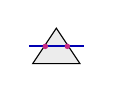
\begin{tikzpicture}[baseline]
            \fill[gray!15] (0, 0) -- (0.6, 0) -- (0.3, 0.45) -- cycle;
            \draw (0, 0) -- (0.6, 0) -- (0.3, 0.45) -- cycle;
            \draw[blue!70!black, thick] (-0.05, 0.22) -- (0.65, 0.22);
            \fill[magenta!80!black] (0.16, 0.22) circle (1pt);
            \fill[magenta!80!black] (0.44, 0.22) circle (1pt);
        \end{tikzpicture}
    };

    \node[stage, right=of s2] (s3) {%
        \textbf{3}\\[-2pt]
        \scriptsize Verkettung\\[2pt]
        
\begin{tikzpicture}[baseline]
            \draw[magenta!80!black, very thick]
                (0.08, 0.10) -- (0.22, 0.05) -- (0.42, 0.05) --
                (0.56, 0.15) -- (0.56, 0.30) -- (0.42, 0.40) --
                (0.22, 0.40) -- (0.08, 0.30) -- cycle;
        \end{tikzpicture}
    };

    % =========================================================
    % Reihe 2: Stufen 4 und 5
    % =========================================================
    \node[stage, below=1.6cm of s1] (s4) {%
        \textbf{4}\\[-2pt]
        \scriptsize Reihenfolge\\[2pt]
        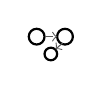
\begin{tikzpicture}[baseline]
            \draw[thick] (0.12, 0.32) circle (0.10);
            \draw[thick] (0.48, 0.32) circle (0.10);
            \draw[thick] (0.30, 0.10) circle (0.08);
            \draw[->, thin, gray!70!black, dashed]
                (0.22, 0.32) -- (0.38, 0.32);
            \draw[->, thin, gray!70!black, dashed]
                (0.45, 0.24) -- (0.36, 0.16);
        \end{tikzpicture}
    };

    \node[stage, right=of s4] (s5) {%
        \textbf{5}\\[-2pt]
        \scriptsize Emission\\[2pt]
        
\begin{tikzpicture}[baseline]
            \draw (0.05, 0) rectangle (0.55, 0.45);
            \foreach \y in {0.10, 0.20, 0.30, 0.38} {
                \draw[gray!60, very thin] (0.10, \y) -- (0.50, \y);
            }
        \end{tikzpicture}
    };

    % =========================================================
    % Pfeile
    % =========================================================
    \draw[flow] (s1) -- (s2);
    \draw[flow] (s2) -- (s3);
    \draw[flow] (s4) -- (s5);

    % =========================================================
    % Umbruch-Pfeil von s3 zu s4
    % WICHTIG: Mittelpunkt zuerst als eigene Coordinate ablegen,
    %          dann |- darauf anwenden.
    % =========================================================
    \coordinate (rowmid) at ($(s1.south)!0.5!(s4.north)$);
    \coordinate (w1) at ([xshift=0.4cm]s3.east);
    \coordinate (w2) at (w1 |- rowmid);
    \coordinate (w3) at (w2 -| s4);
    \draw[flow] (s3.east) -- (w1) -- (w2) -- (w3) -- (s4.north);

    % =========================================================
    % Labels OBERHALB der Pfeile
    % =========================================================
    \node[flowlabel, anchor=south]
        at ([yshift=2pt]$(s1.north east)!0.5!(s2.north west)$)
        {Höhen $a_i$};
    \node[flowlabel, anchor=south]
        at ([yshift=2pt]$(s2.north east)!0.5!(s3.north west)$)
        {Segmente};

    % Wrap-Label im Zwischenraum
    \node[flowlabel]
        at ($(w2)!0.5!(w3)$)
        {Konturringe};

    % Reihe 2
    \node[flowlabel, anchor=south]
        at ([yshift=2pt]$(s4.north east)!0.5!(s5.north west)$)
        {geordnete Ringe};

    % =========================================================
    % Eingabe und Ausgabe
    % =========================================================
    \draw[flow] ([xshift=-0.7cm]s1.west) -- (s1.west);
    \node[iolabel, anchor=east] at ([xshift=-0.75cm]s1.west)
        {\gls{mesh}};

    \draw[flow] (s5.east) -- ([xshift=0.7cm]s5.east);
    \node[iolabel, anchor=west] at ([xshift=0.75cm]s5.east)
        {Schicht-\\datensatz};

\end{tikzpicture}
                    \caption[Verarbeitungspipeline des planaren Algorithmus]{
                        Verarbeitungspipeline des planaren Algorithmus mit fünf zustandslosen Stufen
                    }
                    \label{fig:concept-planar-pipeline}
                \end{figure}

                Die strikte Stufung ist eine bewusste Entscheidung.
                Jede Stufe ist zustandslos, konsumiert ausschließlich die Ausgabe ihrer Vorstufe und erzeugt eine isoliert testbare Repräsentation.
                Dadurch lässt sich die Pipeline stufenweise validieren.
                Zudem ist die spätere Wiederverwendung einzelner Stufen in den nichtplanaren Algorithmen möglich, ohne den planaren Algorithmus als Ganzes verwenden zu müssen.
                Dies gilt insbesondere für das Schnitt- und das Verkettungsverfahren.
                \sig{Adrian Gabriel Axtmann}

            \subsubsection{Schichtpositionen und Mittenversatz}\label{subsubsec:concept-planar-layer-positions}
                Sei $a \in \mathbb{R}$ die skalare Koordinate eines Punktes entlang der \gls{build-axis} $\vec{a}$, d.\,h. die Projektion seiner Ortskoordinate auf $\vec{a}$.
                Mit $a_{\min} = \min_{\vec{v} \in \mathcal{M}} (\vec{v} \cdot \vec{a})$ und $a_{\max} = \max_{\vec{v} \in \mathcal{M}} (\vec{v} \cdot \vec{a})$ werden die kleinste bzw. größte Ausdehnung des Eingabe-\glspl{mesh} $\mathcal{M}$ entlang der \gls{build-axis} bezeichnet.
                $a_i$ ist entsprechend die Höhe der $i$-ten \gls{slice-plane} entlang dieser Achse.
                Die Anzahl der Schichten $N$ ergibt sich aus der Bauteilhöhe $H = a_{\max} - a_{\min}$ entlang der \gls{build-axis} und der parametrierten \gls{layer-height} $t$ als $N = \lceil H / t \rceil$.
                Die zugehörigen Schnitthöhen werden nicht an den Schichtgrenzen, sondern an den Schichtmitten platziert:
                \begin{equation}
                    a_i \;=\; a_{\min} + \left(i + \tfrac{1}{2}\right) \cdot t,
                    \qquad i \in \{0, 1, \dots, N-1\}.
                    \label{eq:concept-planar-layer-positions}
                \end{equation}

                Der konstante Versatz von $\tfrac{1}{2}\,t$ hat einen technischen Hintergrund.
                Eine Platzierung der \glspl{slice-plane} exakt an der unteren oder oberen Grenze einer Schicht würde dazu führen, dass das oberste oder unterste Bauteilfragment in der Höhe einer halben \gls{layer-height} nicht mehr durch eine \gls{slice-plane} erfasst wird.
                Mit dem Mittenversatz hingegen liegt die zugehörige \gls{slice-plane} mittig in jedem Höhenintervall, sodass jedes Bauteilfragment, das mindestens eine halbe \gls{layer-height} hoch ist, in mindestens einer Schicht erscheint.
                Bauteilbereiche, die niedriger als $\tfrac{1}{2}\,t$ sind, sind mit der gewählten \gls{layer-height} physikalisch nicht mehr darstellbar und werden bewusst nicht aufgelöst.
                \sig{Adrian Gabriel Axtmann}

                \begin{figure}[!ht]
                    \centering
                        \begin{tikzpicture}[
    >=Latex,
    scale=0.95,
    every node/.style={font=\small},
]
    % ===========================================
    % PANEL A: Ohne Mittenversatz (links)
    % ===========================================
    \begin{scope}[xshift=0cm]
        % Titel
        \node[font=\bfseries, anchor=south] at (1, 5)
            {(a) An Schichtgrenzen};

        % Aufbauachse a
        \draw[->, thick] (-0.7, -0.3) -- (-0.7, 4.3)
            node[above, font=\scriptsize] {$\vec{a}$};

        % Bauteil (Querschnitt) - Hoehe 3.7 t
        \fill[gray!15] (0, 0) rectangle (1.5, 3.7);
        \draw[thick] (0, 0) rectangle (1.5, 3.7);

        % a_min / a_max Markierungen
        \draw[dotted, thin] (0, 0) -- (-0.85, 0);
        \node[anchor=east, font=\scriptsize] at (-0.85, 0) {$a_{\min}$};
        \draw[dotted, thin] (0, 3.7) -- (-0.85, 3.7);
        \node[anchor=east, font=\scriptsize] at (-0.85, 3.7) {$a_{\max}$};

        % Schichtgrenzen-Hilfslinien
        \foreach \i in {1,2,3} {
            \draw[gray!40, dotted, very thin] (-0.3, \i) -- (2.3, \i);
        }

        % Schnittebenen (an Schichtgrenzen)
        \foreach \y/\i in {0/0, 1/1, 2/2, 3/3} {
            \draw[blue!70!black, very thick] (-0.1, \y) -- (1.6, \y);
            \node[blue!70!black, anchor=west, font=\scriptsize]
                at (1.65, \y) {$a_{\i}$};
        }

        % Nicht erfasster Bereich
        \fill[red!25] (0, 3) rectangle (1.5, 3.7);
        \draw[red!70!black, thick] (0, 3) rectangle (1.5, 3.7);

        % Annotation des fehlenden Fragments
        \node[red!80!black, anchor=south, font=\scriptsize, align=center]
            at (0.75, 4.0) {fehlende Schicht\\($0{,}7\,t$)};

        % Formel
        \node[font=\scriptsize, anchor=north] at (0.75, -0.6)
            {$a_i = a_{\min} + i \cdot t$};
    \end{scope}

    % ===========================================
    % PANEL B: Mit Mittenversatz (rechts)
    % ===========================================
    \begin{scope}[xshift=6cm]
        % Titel
        \node[font=\bfseries, anchor=south] at (1, 5)
            {(b) Mit Mittenversatz};

        % Aufbauachse a
        \draw[->, thick] (-0.7, -0.3) -- (-0.7, 4.3)
            node[above, font=\scriptsize] {$\vec{a}$};

        % Bauteil
        \fill[gray!15] (0, 0) rectangle (1.5, 3.7);
        \draw[thick] (0, 0) rectangle (1.5, 3.7);

        % a_min / a_max
        \draw[dotted, thin] (0, 0) -- (-0.85, 0);
        \node[anchor=east, font=\scriptsize] at (-0.85, 0) {$a_{\min}$};
        \draw[dotted, thin] (0, 3.7) -- (-0.85, 3.7);
        \node[anchor=east, font=\scriptsize] at (-0.85, 3.7) {$a_{\max}$};

        % Schichtgrenzen-Hilfslinien
        \foreach \i in {0,1,2,3,4} {
            \draw[gray!40, dotted, very thin] (-0.3, \i) -- (2.3, \i);
        }

        % Schnittebenen (mittig)
        \foreach \y/\i in {0.5/0, 1.5/1, 2.5/2, 3.5/3} {
            \draw[green!50!black, very thick] (-0.1, \y) -- (1.6, \y);
            \node[green!50!black, anchor=west, font=\scriptsize]
                at (1.65, \y) {$a_{\i}$};
        }

        % Bewusst akzeptierter Restbereich (klein)
        \fill[gray!40] (0, 3.5) rectangle (1.5, 3.7);

        % Annotation
        \node[gray!60!black, anchor=south, font=\scriptsize, align=center]
            at (0.75, 4.0) {$<\tfrac{t}{2}$ (akzeptiert)};

        % t/2 und t Bemassung innerhalb des Bauteils
        \draw[<->, thin, blue!70!black] (0.15, 0) -- (0.15, 0.5);
        \node[anchor=west, font=\scriptsize, blue!70!black]
            at (0.18, 0.25) {$\tfrac{t}{2}$};
        \draw[<->, thin, blue!70!black] (0.15, 0.5) -- (0.15, 1.5);
        \node[anchor=west, font=\scriptsize, blue!70!black]
            at (0.18, 1.0) {$t$};

        % Formel
        \node[font=\scriptsize, anchor=north] at (0.75, -0.6)
            {$a_i = a_{\min} + (i+\tfrac{1}{2}) \cdot t$};
    \end{scope}
\end{tikzpicture}

                    \caption[Mittenversatz der Schnittebenen im planaren Algorithmus]{
                        Vergleich zweier Platzierungsvarianten der Schnittebenen.
                        (a)~Platzierung an den Schichtgrenzen: das oberste Fragment bleibt unberücksichtigt.
                        (b)~Mittenversatz nach \cref{eq:concept-planar-layer-positions}: jedes Fragment ab $\tfrac{t}{2}$ Höhe erscheint in genau einer Schicht.
                    }
                    \label{fig:concept-planar-mid-offset}
                \end{figure}

            \subsubsection{Geometrische Grundoperation: Ebene-Mesh-Schnitt}\label{subsubsec:concept-planar-plane-intersection} \index{Schnittoperation!Ebene-Dreieck}
                Die zentrale geometrische Grundoperation ist der Schnitt einer \gls{slice-plane} mit einem einzelnen \gls{triangle}.
                Für jede Schicht $i$ wird über alle \glspl{triangle} des Eingabe-\glspl{mesh} iteriert.
                Pro \gls{triangle} wird der vorzeichenbehaftete Abstand $d_j = (\vec{v}_j)_a - a_i$ jedes \gls{vertex} $\vec{v}_j$ zur \gls{slice-plane} berechnet.
                Das Vorzeichen von $d_j$ kodiert dabei die Lage des \glspl{vertex} relativ zur \gls{slice-plane}: $d_j > 0$ bedeutet oberhalb, $d_j < 0$ unterhalb und $d_j = 0$ exakt auf der Ebene.

                Eine \gls{edge} zwischen zwei \glspl{vertex} $\vec{v}_A$ und $\vec{v}_B$ schneidet die \gls{slice-plane} genau dann, wenn die Vorzeichen der zugehörigen Abstände verschieden sind, formal $\operatorname{sgn}(d_A) \neq \operatorname{sgn}(d_B)$, wobei $\operatorname{sgn}$ die Signumfunktion bezeichnet.
                Anschaulich entspricht dies der Aussage, dass ein Endpunkt der \gls{edge} oberhalb und der andere unterhalb der \gls{slice-plane} liegen muss, sodass die \gls{edge} die Ebene zwangsläufig durchquert.
                Der Schnittpunkt $\vec{P}$ ergibt sich aus linearer Interpolation entlang der \gls{edge}:
                \begin{equation}
                    \vec{P} \;=\; \vec{v}_A + \tau \cdot (\vec{v}_B - \vec{v}_A),
                    \qquad
                    \tau \;=\; \frac{d_A}{d_A - d_B} \;\in\; [0, 1].
                    \label{eq:concept-planar-edge-intersection}
                \end{equation}
                Der Interpolationsparameter $\tau$ gibt an, an welcher relativen Position entlang der \gls{edge} die \gls{slice-plane} durchstoßen wird: $\tau = 0$ entspricht $\vec{v}_A$, $\tau = 1$ entspricht $\vec{v}_B$, und $\tau = \tfrac{1}{2}$ liegt genau in der Mitte.
                Die Formel ist die direkte Lösung der Gleichung $d_A + \tau \cdot (d_B - d_A) = 0$ und liefert damit denjenigen Punkt, an dem der vorzeichenbehaftete Abstand zur \gls{slice-plane} gerade null wird.
                Da ein \gls{triangle} unter den hier betrachteten Voraussetzungen höchstens an zwei \glspl{edge} geschnitten wird, liefert es maximal ein \gls{line-segment} pro Schicht.

                \begin{figure}[!ht]
                    \centering
                    \begin{tikzpicture}[
    >=Latex,
    scale=1.0,
    every node/.style={font=\small},
]
    % ===========================================
    % Aufbauachse a (links)
    % ===========================================
    \draw[->, thick] (-1.0, -0.4) -- (-1.0, 4.6)
        node[above, font=\scriptsize] {$\vec{a}$};

    % ===========================================
    % Schnittebene a_i (duenner halbtransparenter Band)
    % ===========================================
    \fill[blue!12, opacity=0.5] (-0.6, 1.95) rectangle (6.2, 2.05);
    \draw[blue!70!black, thick] (-0.6, 2.0) -- (6.2, 2.0);
    \node[blue!70!black, anchor=west, font=\scriptsize]
        at (6.25, 2.0) {Schnittebene $a_i$};

    % ===========================================
    % Dreieck mit drei Vertices
    % ===========================================
    \coordinate (v1) at (1.0, 3.8);
    \coordinate (v2) at (3.0, 0.3);
    \coordinate (v3) at (5.4, 3.4);

    \fill[gray!12] (v1) -- (v2) -- (v3) -- cycle;
    \draw[thick] (v1) -- (v2) -- (v3) -- cycle;

    % Schnittpunkte (linear berechnet)
    \coordinate (Pa) at (2.029, 2.0);
    \coordinate (Pb) at (4.316, 2.0);

    % Resultierendes Liniensegment (Magenta hervorgehoben)
    \draw[magenta!80!black, very thick, line width=2pt] (Pa) -- (Pb);

    % Vertices als Kreise
    \fill[red!70!black] (v1) circle (2.5pt);
    \fill[blue!70!black] (v2) circle (2.5pt);
    \fill[red!70!black] (v3) circle (2.5pt);

    % Vertex-Labels: alle ausserhalb des Dreiecks platziert
    \node[anchor=south west, font=\scriptsize] at ($(v1)+(0.10, 0.05)$)
        {$\vec{v}_1\;(d_1>0)$};
    \node[anchor=north, font=\scriptsize] at ($(v2)+(0, -0.18)$)
        {$\vec{v}_2\;(d_2<0)$};
    \node[anchor=south west, font=\scriptsize] at ($(v3)+(0.10, 0.05)$)
        {$\vec{v}_3\;(d_3>0)$};

    % ===========================================
    % Dimensionspfeil d_1 (weit LINKS vom Dreieck)
    % ===========================================
    \coordinate (D1top) at (0.3, 3.8);
    \coordinate (D1bot) at (0.3, 2.0);
    \draw[red!50!black, thin, dotted] (D1top) -- (v1);
    \draw[<->, thin, red!70!black] (D1top) -- (D1bot);
    \node[red!70!black, anchor=east, font=\scriptsize]
        at ($(D1top)!0.5!(D1bot)+(-0.05, 0)$) {$|d_1|$};

    % ===========================================
    % Dimensionspfeil |d_2| (RECHTS unten, ausserhalb des Dreiecks)
    % ===========================================
    \coordinate (D2bot) at (4.6, 0.3);
    \coordinate (D2top) at (4.6, 2.0);
    \draw[blue!50!black, thin, dotted] (v2) -- (D2bot);
    \draw[<->, thin, blue!70!black] (D2bot) -- (D2top);
    \node[blue!70!black, anchor=west, font=\scriptsize]
        at ($(D2bot)!0.5!(D2top)+(0.05, 0)$) {$|d_2|$};

    % ===========================================
    % Schnittpunkt-Marker und Labels (klar OBERHALB des Bands)
    % ===========================================
    \fill[magenta!80!black] (Pa) circle (2.5pt);
    \fill[magenta!80!black] (Pb) circle (2.5pt);
    \node[magenta!80!black, anchor=south west, font=\scriptsize]
        at ($(Pa)+(0.05, 0.18)$) {$\vec{P}_A$};
    \node[magenta!80!black, anchor=south east, font=\scriptsize]
        at ($(Pb)+(-0.05, 0.18)$) {$\vec{P}_B$};

    % ===========================================
    % Dashed Linie v1 -> Pa mit tau-Label
    % tau im Dreieck-Inneren, abseits von d_1
    % ===========================================
    \draw[->, thin, gray!70!black, dashed] (v1) -- (Pa);
    \node[gray!50!black, font=\scriptsize, anchor=south west]
        at ($(v1)!0.5!(Pa)+(0.18, 0.10)$) {$\tau$};

    % ===========================================
    % Formel am unteren Rand
    % ===========================================
    \node[font=\scriptsize, anchor=north] at (3.0, -0.95)
        {$\vec{P} = \vec{v}_A + \tau\,(\vec{v}_B - \vec{v}_A),
          \quad \tau = d_A/(d_A - d_B)$};
\end{tikzpicture}
                    \caption[Ebene-Dreieck-Schnitt mit linearer Kanteninterpolation]{
                        Schnitt einer Schichtebene $a_i$ mit einem Dreieck ($d_1 > 0$, $d_2 < 0$, $d_3 > 0$).
                        Die vorzeichenwechselnden Kanten werden nach \cref{eq:concept-planar-edge-intersection} geschnitten; das verbindende Segment (magenta) bildet den Kontur-Beitrag.
                    }
                    \label{fig:concept-planar-plane-triangle}
                \end{figure}

                Es sind drei Sonderfälle zu betrachten, die alle aus der Lage von \glspl{vertex} oder ganzen \glspl{edge} exakt auf der \gls{slice-plane} resultieren:

                \begin{description}
                    \item[Eckpunkt auf der Ebene]
                    Liegt ein \gls{vertex} exakt auf der \gls{slice-plane}, so melden zwei benachbarte \glspl{edge} denselben Punkt als Schnittpunkt, was zu einer doppelten Erfassung und damit zu einem entarteten \gls{line-segment} führen würde.
                    Die Doppelzählung wird dadurch vermieden, dass ein Schnitt nur dann gezählt wird, wenn der \gls{vertex} am Anfang der betrachteten \gls{edge} liegt.
                    An der angrenzenden \gls{edge}, an der derselbe \gls{vertex} am Ende steht, wird der Schnitt unterdrückt.
                    \item[\Gls{edge} auf der Ebene]
                    Liegen beide Endpunkte einer \gls{edge} auf der \gls{slice-plane}, so erfasst die a-Endpunkt-Regel beide \glspl{vertex} einzeln.
                    Den ersten als Startpunkt der koplanaren \gls{edge}, den zweiten als Startpunkt der anschließenden \gls{edge}.
                    Das resultierende \gls{line-segment} entspricht damit geometrisch der koplanaren \gls{edge} selbst und wird wie ein reguläres Schnittsegment in die nachfolgende Verkettungsstufe übergeben.
                    \item[\Gls{triangle} auf der Ebene]
                    Liegen alle drei \glspl{vertex} eines \glspl{triangle} auf der \gls{slice-plane}, so werden die ersten beiden \glspl{vertex} in der Reihenfolge der \gls{face}-\gls{vertex}-Liste durch die a-Endpunkt-Regel erfasst.
                    Die Auswertung der dritten \gls{edge} wird durch die Kapazitätsobergrenze $n = 2$ unterdrückt.
                    Das entstehende \gls{line-segment} gibt damit eine Kante des koplanaren \glspl{triangle} wieder.
                    Da koplanare \glspl{triangle} bei \gls{watertight}[en] \glspl{mesh} in der Praxis nicht auftreten, hat dieser Fall keinen Einfluss auf die Korrektheit der Pipeline.
                \end{description}

                \begin{figure}[ht]
                    \centering
                    \resizebox{\linewidth}{!}{%
                        \begin{tikzpicture}[
    >=Latex,
    scale=0.85,
    every node/.style={font=\small},
]
    % ============================================================
    % PANEL A: Eckpunkt auf Ebene
    % ============================================================
    \begin{scope}[xshift=0cm]
        \node[font=\bfseries, anchor=south] at (2.0, 4.5)
            {(a) Eckpunkt auf Ebene};

        % Schnittebene
        \fill[blue!12, opacity=0.5] (-0.3, 1.95) rectangle (4.3, 2.05);
        \draw[blue!70!black, thick] (-0.3, 2.0) -- (4.3, 2.0);
        \node[blue!70!black, anchor=west, font=\tiny]
            at (4.3, 2.0) {Ebene};

        % Triangle: V auf Ebene, A oben, B unten
        \coordinate (V) at (0.6, 2.0);
        \coordinate (A) at (3.2, 3.5);
        \coordinate (B) at (3.2, 0.5);
        \coordinate (P) at (3.2, 2.0);

        \fill[gray!12] (V) -- (A) -- (B) -- cycle;
        \draw[thick] (V) -- (A) -- (B) -- cycle;

        % Resultierendes Schnittsegment V-P
        \draw[magenta!80!black, very thick, line width=2pt] (V) -- (P);

        % Marker
        \fill[red!70!black] (A) circle (2pt);
        \fill[blue!70!black] (B) circle (2pt);
        \fill[red!80!black] (V) circle (3.5pt);
        \fill[magenta!80!black] (P) circle (2.5pt);

        % Vertex-Labels: alle klar AUSSERHALB des Triangles
        \node[anchor=west, font=\scriptsize] at ($(A)+(0.15, 0)$)
            {$\vec{A}\;(d{>}0)$};
        \node[anchor=west, font=\scriptsize] at ($(B)+(0.15, 0)$)
            {$\vec{B}\;(d{<}0)$};
        \node[red!80!black, anchor=east, font=\scriptsize]
            at ($(V)+(0, 0.5)$) {$\vec{V}\;(d{=}0)$};
        \node[magenta!80!black, anchor=south west, font=\scriptsize]
            at ($(P)+(0.05, 0.15)$) {$\vec{P}$};

        % Annotationen "Kante V-A meldet V" und "Kante V-B meldet V"
        \node[red!50!black, font=\tiny, anchor=south east, align=center]
            at (1.7, 3.5) {Kante $\vec{V}\!\to\!\vec{A}$\\meldet $\vec{V}$};
        \draw[->, thin, red!50!black]
            (1.4, 3.65) to[out=-90, in=60] ($(V)+(0.18, 0.18)$);

        \node[red!50!black, font=\tiny, anchor=north east, align=center]
            at (1.7, 0.5) {Kante $\vec{V}\!\to\!\vec{B}$\\meldet $\vec{V}$};
        \draw[->, thin, red!50!black]
            (1.4, 0.35) to[out=90, in=-60] ($(V)+(0.18, -0.18)$);

        % Erklärung unten (Rechtschreibung korrigiert)
        \node[anchor=north, font=\scriptsize, align=center] at (2.0, -0.45)
            {\textbf{Problem:} $\vec{V}$ doppelt erfasst.\\
             \textbf{Regel:} nur die Kante zählen,\\
             an der $\vec{V}$ \emph{Anfang} ist.};
    \end{scope}

    % ============================================================
    % PANEL B: Kante auf Ebene
    % ============================================================
    \begin{scope}[xshift=6.0cm]
        \node[font=\bfseries, anchor=south] at (2.0, 4.5)
            {(b) Kante auf Ebene};

        \fill[blue!12, opacity=0.5] (-0.3, 1.95) rectangle (4.3, 2.05);
        \draw[blue!70!black, thick] (-0.3, 2.0) -- (4.3, 2.0);
        \node[blue!70!black, anchor=west, font=\tiny]
            at (4.3, 2.0) {Ebene};

        \coordinate (TA) at (0.7, 2.0);
        \coordinate (TB) at (3.3, 2.0);
        \coordinate (TC) at (2.0, 3.5);

        \fill[gray!12] (TA) -- (TB) -- (TC) -- cycle;
        \draw[thick] (TA) -- (TC) -- (TB) -- cycle;

        % Koplanare Kante orange
        \draw[orange!85!black, very thick, dash pattern=on 5pt off 2pt,
              line width=1.5pt] (TA) -- (TB);

        \fill[red!80!black] (TA) circle (3pt);
        \fill[red!80!black] (TB) circle (3pt);
        \fill[red!70!black] (TC) circle (2pt);

        \node[anchor=south, font=\scriptsize] at ($(TC)+(0, 0.1)$)
            {$\vec{C}\;(d{>}0)$};
        \node[red!80!black, anchor=north east, font=\scriptsize]
            at ($(TA)+(-0.05, -0.1)$) {$\vec{A}\;(d{=}0)$};
        \node[red!80!black, anchor=north west, font=\scriptsize]
            at ($(TB)+(0.05, -0.1)$) {$\vec{B}\;(d{=}0)$};

        % Annotation OBERHALB des Triangles, Pfeil zur orangen Kante
        \node[orange!85!black, font=\tiny, anchor=south, align=center]
            at (3.6, 2.95) {Kante $\vec{A}\vec{B}$\\koplanar};
        \draw[->, thin, orange!85!black]
            (3.4, 2.85) to[out=-135, in=20] ($(TA)!0.65!(TB)+(0, 0.08)$);

        \node[anchor=north, font=\scriptsize, align=center] at (2.0, -0.45)
            {\textbf{Problem:} keine eindeutige\\
             Punktinformation, $\vec{A}\vec{B}$ ist tangential.\\
             \textbf{Regel:} Kante stillschweigend ignorieren.};
    \end{scope}

    % ============================================================
    % PANEL C: Dreieck auf Ebene
    % ============================================================
    \begin{scope}[xshift=12.0cm]
        \node[font=\bfseries, anchor=south] at (2.0, 4.5)
            {(c) Dreieck auf Ebene};

        % 3D-Parallelogramm
        \fill[blue!12, opacity=0.6]
            (0.0, 1.4) -- (4.0, 1.4) -- (3.4, 2.8) -- (-0.6, 2.8) -- cycle;
        \draw[blue!70!black, thick]
            (0.0, 1.4) -- (4.0, 1.4) -- (3.4, 2.8) -- (-0.6, 2.8) -- cycle;
        
        \node[blue!70!black, anchor=west, font=\tiny]
            at (4.0, 1.4) {Ebene};

        % Triangle ON the plane
        \coordinate (CA) at (0.5, 1.7);
        \coordinate (CB) at (3.0, 1.7);
        \coordinate (CC) at (1.5, 2.5);

        \fill[gray!40, opacity=0.7] (CA) -- (CB) -- (CC) -- cycle;
        \draw[gray!60!black, thick] (CA) -- (CB) -- (CC) -- cycle;

        \fill[red!70!black] (CA) circle (2.5pt);
        \fill[red!70!black] (CB) circle (2.5pt);
        \fill[red!70!black] (CC) circle (2.5pt);

        \node[gray!40!black, font=\scriptsize\itshape] at (1.66, 1.96)
            {koplanar};

        % Linkes Label ist jetzt bei x=-0.8 (deutlich außerhalb des blauen Rahmens)
        \node[red!70!black, anchor=east, font=\scriptsize] (lblCA)
            at (0.5, 1.0) {$d{=}0$};
        \draw[thin, red!70!black] (lblCA.east) -- (CA);

        % Rechtes Label ist jetzt bei x=4.2 (deutlich außerhalb des blauen Rahmens)
        \node[red!70!black, anchor=west, font=\scriptsize] (lblCB)
            at (4.2, 1.7) {$d{=}0$};
        \draw[thin, red!70!black] (lblCB.west) -- (CB);

        \node[red!70!black, anchor=south, font=\scriptsize] (lblCC)
            at (1.5, 3.0) {$d{=}0$};
        \draw[thin, red!70!black] (lblCC.south) -- (CC);

        % Erklärung unten (Rechtschreibung korrigiert)
        \node[anchor=north, font=\scriptsize, align=center] at (2.0, -0.45)
            {\textbf{Problem:} keine 1D-Kontur,\\
             nur eine 2D-Fläche.\\
             \textbf{Regel:} verwerfen, Nachbardreiecke\\
             liefern bereits die Kontur.};
    \end{scope}
\end{tikzpicture}
                    }
                    \caption[Sonderfälle des Ebene-Dreieck-Schnitts]{
                        Drei Sonderfälle des Ebene-Dreieck-Schnitts\\
                        (a)~Liegt ein Vertex $\vec{v}$ exakt auf der Ebene, würden zwei benachbarte Dreiecke denselben Punkt melden. Der Schnitt wird nur an derjenigen Edge gezählt, an der $\vec{v}$ am Anfang steht.
                        (b)~Liegt eine ganze \gls{edge} auf der Ebene, ist sie tangential und wird ignoriert.
                        (c)~Liegen alle drei Vertizes eines Dreiecks auf der Ebene, ist es koplanar. Es wird vollständig verworfen, da die umlaufenden Nachbardreiecke die Kontur bereits abbilden.%
                    }
                    \label{fig:concept-planar-special-cases}
                \end{figure}

                Diese Fallunterscheidung ist nicht nur ein Implementierungsdetail, sondern eine Voraussetzung dafür, dass die nachgelagerte Verkettungsstufe wohlgeformte Eingabedaten erhält.
                Ohne sie würden Punktduplikate und Null-\glspl{line-segment} die Verkettung erschweren und zu fehlerhaften Konturen führen.
                \sig{Adrian Gabriel Axtmann}

            \subsubsection{Verkettung der Segmente zu Konturringen}\label{subsubsec:concept-planar-contour-chaining} \index{Kontur!Verkettung}
                Die in der Schnittstufe gewonnenen \glspl{line-segment} sind topologisch unsortiert und müssen zu geschlossenen \glspl{polygonal-chain}[n], im Folgenden \glspl{contour-ring} genannt, verkettet werden.
                Dies ist notwendig, da die spätere \gls{path-planning} in \ac{kronos} jede Kontur als zusammenhängenden Bewegungsbefehl ausführt.
                Nur in einer geordneten Schleife kann der Druckkopf die Bauteilbegrenzung in einem ununterbrochenen Bewegungsablauf abfahren.

                Die Verkettung wird als \emph{gieriges \gls{nearest-neighbor}} formuliert.
                Das Verfahren beginnt an einem beliebigen, noch unbenutzten Start-\gls{line-segment} und führt einen \emph{Cursor} mit, der die aktuelle Position am Ende des bisher aufgebauten Rings markiert.
                In jedem Schritt werden die Endpunkte aller noch unbenutzten \glspl{line-segment} betrachtet, und dasjenige \gls{line-segment} wird angefügt, dessen näherer Endpunkt den minimalen euklidischen Abstand zum Cursor besitzt.
                Liegt der nähere Endpunkt am hinteren Ende eines \gls{line-segment}[s], so wird das \gls{line-segment} vor dem Anfügen umgedreht, sodass der Ring durchgängig in eine Richtung wächst.
                Anschließend wird der Cursor an das jetzt freie Ende des angefügten \gls{line-segment}[s] weitergesetzt.
                Der Ring gilt als geschlossen, sobald der Cursor wieder in eine Toleranzumgebung des Startpunkts zurückgekehrt ist.
                Das Verfahren ist \emph{gierig} (engl. \emph{greedy}), da es in jedem Schritt ausschließlich die lokal beste Entscheidung trifft, also den nächsten Nachbarn wählt, ohne die globalen Auswirkungen dieser Wahl auf den weiteren Ringverlauf zu berücksichtigen.

                \begin{figure}[ht]
                    \centering
                    \begin{tikzpicture}[
    >=Latex,
    scale=0.85,
    every node/.style={font=\small},
]
    % ============================================================
    % PANEL A: Unsortierte Segmente
    % ============================================================
    \begin{scope}[xshift=0cm, yshift=0cm]
        \node[font=\bfseries, anchor=south] at (2.0, 4.2)
            {(a) Unsortierte Segmente};

        % 7 Segmente mit Luecken (shorten)
        \draw[gray!70, thick, ->, shorten >=3pt, shorten <=3pt]
            (0.6, 1.0) -- (1.8, 0.6);
        \draw[gray!70, thick, ->, shorten >=3pt, shorten <=3pt]
            (3.6, 2.6) -- (3.0, 3.4);
        \draw[gray!70, thick, ->, shorten >=3pt, shorten <=3pt]
            (1.8, 0.6) -- (3.2, 0.8);
        \draw[gray!70, thick, ->, shorten >=3pt, shorten <=3pt]
            (1.4, 3.2) -- (0.6, 2.4);
        \draw[gray!70, thick, ->, shorten >=3pt, shorten <=3pt]
            (3.6, 2.6) -- (3.2, 0.8);   % wird in (c) umgedreht
        \draw[gray!70, thick, ->, shorten >=3pt, shorten <=3pt]
            (3.0, 3.4) -- (1.4, 3.2);
        \draw[gray!70, thick, ->, shorten >=3pt, shorten <=3pt]
            (0.6, 2.4) -- (0.6, 1.0);

        % Endpunkt-Marker zeigen, dass es 7 isolierte Segmente sind
        \foreach \p in {(0.6, 1.0), (1.8, 0.6), (3.2, 0.8), (3.6, 2.6),
                        (3.0, 3.4), (1.4, 3.2), (0.6, 2.4)} {
            \fill[gray!90!black] \p circle (1.5pt);
        }

        \node[anchor=north, font=\scriptsize, align=center] at (2.0, -0.2)
            {7 Segmente, beliebige\\
             Speicherreihenfolge und\\
             Ausrichtung};
    \end{scope}

    % ============================================================
    % PANEL B: Wahl Startsegment + Cursor
    % ============================================================
    \begin{scope}[xshift=6cm, yshift=0cm]
        \node[font=\bfseries, anchor=south] at (2.0, 4.2)
            {(b) Startsegment};

        % Inaktive Segmente
        \draw[gray!40, thick] (3.6, 2.6) -- (3.0, 3.4);
        \draw[gray!40, thick] (1.8, 0.6) -- (3.2, 0.8);
        \draw[gray!40, thick] (1.4, 3.2) -- (0.6, 2.4);
        \draw[gray!40, thick] (3.6, 2.6) -- (3.2, 0.8);
        \draw[gray!40, thick] (3.0, 3.4) -- (1.4, 3.2);
        \draw[gray!40, thick] (0.6, 2.4) -- (0.6, 1.0);

        % Startsegment in Magenta
        \draw[magenta!80!black, very thick, ->] (0.6, 1.0) -- (1.8, 0.6);
        \fill[magenta!80!black] (0.6, 1.0) circle (3pt);
        \node[magenta!80!black, anchor=east, font=\scriptsize]
            at (0.45, 1.0) {Start};

        % Cursor am freien Ende
        \fill[red!70!black] (1.8, 0.6) circle (3.5pt);
        \draw[red!70!black, thick] (1.8, 0.6) circle (5.5pt);
        \node[red!70!black, anchor=north west, font=\scriptsize]
            at (1.95, 0.40) {Cursor};

        \node[anchor=north, font=\scriptsize, align=center] at (2.0, -0.2)
            {Beliebiges Startsegment\\
             gewählt; Cursor markiert\\
             das freie Ende};
    \end{scope}

    % ============================================================
    % PANEL C: Iteration mit Umdrehen
    % ============================================================
    \begin{scope}[xshift=0cm, yshift=-7cm]
        \node[font=\bfseries, anchor=south] at (2.0, 4.2)
            {(c) Segment umkehren};

        % Bisheriger Ringverlauf in Magenta
        \draw[magenta!80!black, very thick, ->] (0.6, 1.0) -- (1.8, 0.6);
        \draw[magenta!80!black, very thick, ->] (1.8, 0.6) -- (3.2, 0.8);

        % Cursor am aktuellen Ende
        \fill[red!70!black] (3.2, 0.8) circle (3.5pt);
        \draw[red!70!black, thick] (3.2, 0.8) circle (5.5pt);

        % Originalrichtung (gestrichelt grau, LINKS versetzt)
        \draw[gray!50, thick, dashed, ->]
            ($(3.6, 2.6)+(-0.14, 0.03)$) -- ($(3.2, 0.8)+(-0.14, 0.03)$);

        % Umgedrehte Richtung (orange, RECHTS versetzt)
        \draw[orange!80!black, very thick, ->]
            ($(3.2, 0.8)+(0.14, -0.03)$) -- ($(3.6, 2.6)+(0.14, -0.03)$);

        % Restliche Segmente grau
        \draw[gray!40, thick] (3.6, 2.6) -- (3.0, 3.4);
        \draw[gray!40, thick] (1.4, 3.2) -- (0.6, 2.4);
        \draw[gray!40, thick] (3.0, 3.4) -- (1.4, 3.2);
        \draw[gray!40, thick] (0.6, 2.4) -- (0.6, 1.0);

        % Annotation "original" - INNEN im Ring
        \node[gray!50!black, anchor=east, font=\scriptsize]
            at (2.8, 2.0) {original};
        \draw[gray!50!black, thin]
            (2.85, 2.0) to[bend right=10] (3.25, 1.7);

        \node[orange!80!black, anchor=west, font=\scriptsize]
            at (3.9, 2.4) {umkehren};
        \draw[orange!80!black, ->, thick]
            (4.0, 1.5) -- (4.2, 1.5) arc[start angle=-90, end angle=90, radius=0.25] -- (4.0, 2.0);

        \node[anchor=north, font=\scriptsize, align=center] at (2.0, -0.2)
            {Näherer Endpunkt liegt am\\
             hinteren Ende $\Rightarrow$ Segment\\
             vor Anfügen umkehren};
    \end{scope}

    % ============================================================
    % PANEL D: Geschlossener Ring + Snap-Tolerance
    % ============================================================
    \begin{scope}[xshift=6cm, yshift=-7cm]
        \node[font=\bfseries, anchor=south] at (2.0, 4.2)
            {(d) Geschlossener Ring};

        % Startpunkt-Marker
        \fill[magenta!80!black] (0.6, 1.0) circle (3pt);

        % Toleranzkreis um Startpunkt
        \draw[red!70!black, thick, dashed] (0.6, 1.0) circle (11pt);

        \node[red!70!black, anchor=east, font=\scriptsize, align=center]
            at (0.2, 0.2) {Snap-Tolerance\\$\varepsilon$};
        \draw[red!70!black, ->, thin]
            (-0.25, 0.7) to[out=45, in=200] (0.25, 0.9);

        \node[anchor=north, font=\scriptsize, align=center] at (2.0, -0.2)
            {Cursor in $\varepsilon$-Umgebung\\
             des Startpunkts\\
             $\Rightarrow$ Ring schließt};

        % Vollstaendiger Ring in Magenta
        \draw[magenta!80!black, very thick, ->] (0.6, 1.0) -- (1.8, 0.6);
        \draw[magenta!80!black, very thick, ->] (1.8, 0.6) -- (3.2, 0.8);
        \draw[magenta!80!black, very thick, ->] (3.2, 0.8) -- (3.6, 2.6);
        \draw[magenta!80!black, very thick, ->] (3.6, 2.6) -- (3.0, 3.4);
        \draw[magenta!80!black, very thick, ->] (3.0, 3.4) -- (1.4, 3.2);
        \draw[magenta!80!black, very thick, ->] (1.4, 3.2) -- (0.6, 2.4);
        \draw[magenta!80!black, very thick, ->] (0.6, 2.4) -- (0.5, 1.2);
    \end{scope}
\end{tikzpicture}
                    \caption[Greedy-Nearest-Neighbor-Verkettung der Schnittsegmente]{
                        Gierige Verkettung der Schnittsegmente zu einem geschlossenen Konturring.
                        (a)~Unsortierte Segmente.
                        (b)~Wahl eines Startsegments.
                        (c)~Iteratives Anfügen des nächsten Segments.
                        (d)~Ringschluss bei Rückkehr in die $\varepsilon$-Umgebung (\gls{snap-tolerance}) des Startpunkts.
                    }
                    \label{fig:concept-planar-chaining}
                \end{figure}

                Die Wahl dieses Verfahrens ist ein bewusster Kompromiss.
                Bei einem \gls{watertight}[en] \gls{mesh} besitzt jeder Schnittpunkt genau einen Nachbarn auf derselben gemeinsamen \gls{mesh}-\gls{edge}, sodass das gierige \gls{nearest-neighbor} stets den geometrisch korrekten Nachfolger findet und mit dem globalen Optimum zusammenfällt.
                Eine aufwändigere Optimierung (etwa über das \gls{traveling-salesman-problem}) brächte daher keinen Mehrwert.
                Eine schnellere Verkettung über die \gls{mesh}-Adjazenzlisten würde dagegen die Wiederverwendung der Stufe in den nichtplanaren Algorithmen verhindern, deren \glspl{line-segment} keine eindeutige Nachbarschaftsinformation mehr besitzen.

                Die Toleranzumgebung, im Folgenden als \gls{snap-tolerance} bezeichnet, ist erforderlich, da zwei numerisch berechnete Schnittpunkte auf derselben gemeinsamen \gls{mesh}-\gls{edge} zwar in der Regel exakt übereinstimmen, durch Rundung in \gls{ieee-754}-Arithmetik aber leicht abweichen können.
                Die Toleranz ist gleichzeitig so gering zu wählen, dass tatsächlich verschiedene Punkte nicht fälschlich zusammenfallen und so groß, dass numerisches Rauschen sicher überdeckt wird.

                Eine Schicht kann mehrere voneinander unabhängige \glspl{contour-ring} enthalten, z.\,B. bei Bauteilen mit Bohrungen oder bei mehreren auf der \gls{buildplate} angeordneten Teilen.
                Das Verfahren wird daher so lange wiederholt, bis alle \glspl{line-segment} verbraucht sind.
                Verbleibt am Ende ein offener \gls{polygonal-chain}, deutet dies auf ein nicht-mannigfaltiges \gls{mesh} hin.
                Die Implementierung nimmt solche Teilketten dennoch in die Ringliste auf, sofern sie mindestens zwei Punkte umfassen.
                Eine explizite Verwerfung findet nicht statt.
                Dies ist vertretbar, weil bei korrekten \gls{watertight}[en]-\glspl{mesh} keine offenen Ketten entstehen.
                \sig{Adrian Gabriel Axtmann}

            \subsubsection{Reihenfolge der Konturringe innerhalb einer Schicht}\label{subsubsec:concept-planar-ring-ordering}
                Enthält eine Schicht mehr als einen \gls{contour-ring}, so beeinflusst die Reihenfolge ihrer Abarbeitung den notwendigen Verbindungsweg zwischen den Ringen sowie die Druckqualität.
                Lange Verbindungswege zwischen disjunkten Konturen verlängern die Fertigungsdauer und erhöhen die Wahrscheinlichkeit unerwünschter Materialfäden zwischen den Konturen.

                Die Reihenfolge wird daher als Annäherung an das \gls{traveling-salesman-problem} aufgefasst, beschränkt auf die \glspl{contour-ring} einer einzelnen Schicht.
                Da die Anzahl der Ringe pro Schicht bei den hier betrachteten Bauteilen typischerweise im einstelligen Bereich liegt, ist eine exakte Lösung des Problems unverhältnismäßig aufwendig.
                Stattdessen wird ein gieriges \gls{nearest-neighbor} eingesetzt.
                Als Startring wird derjenige Ring gewählt, dessen geometrischer Schwerpunkt den kleinsten Wert entlang der horizontalen Achse aufweist; dadurch beginnt die Roboterbewegung nahe am Koordinatenursprung.
                Ausgehend von diesem Startring wird stets derjenige unbearbeitete Ring angefügt, dessen Anfangs- oder Endpunkt dem aktuellen Cursor am nächsten liegt.
                Liegt der Endpunkt näher als der Anfangspunkt, wird der Ring umgekehrt durchlaufen, da die Konturrichtung das gedruckte Ergebnis nicht verändert, wohl aber die Länge des Verbindungswegs zum nächsten Ring.

                \begin{figure}[ht]
                    \centering
                    \begin{tikzpicture}[
    >=Latex,
    scale=0.9,
    every node/.style={font=\small},
]
    % ===========================================
    % Gemeinsame Geometrie pro Panel:
    %   - Aussenring eines Bauteils (gross)
    %   - Drei Bohrungen (kleine Kreise)
    %   - Ein zweites Bauteil daneben
    % Eintrittspunkte werden pro Ring markiert.
    % ===========================================

    % ============== PANEL A ==============
    \begin{scope}[xshift=0cm]
        \node[font=\bfseries, anchor=south] at (3.0, 5.0)
            {(a) Schlechte Reihenfolge};

        % Aussenkontur Bauteil 1 (links)
        \draw[thick] (0.4, 0.6) rectangle (3.4, 4.2);
        \fill[gray!10] (0.4, 0.6) rectangle (3.4, 4.2);
        \draw[thick] (0.4, 0.6) rectangle (3.4, 4.2);

        % Drei Bohrungen
        \fill[white] (1.2, 1.4) circle (0.35);
        \draw[thick] (1.2, 1.4) circle (0.35);
        \fill[white] (2.6, 1.4) circle (0.35);
        \draw[thick] (2.6, 1.4) circle (0.35);
        \fill[white] (1.9, 3.2) circle (0.4);
        \draw[thick] (1.9, 3.2) circle (0.4);

        % Bauteil 2 (rechts)
        \draw[thick] (4.6, 1.6) rectangle (5.8, 3.4);
        \fill[gray!10] (4.6, 1.6) rectangle (5.8, 3.4);
        \draw[thick] (4.6, 1.6) rectangle (5.8, 3.4);

        % Eintrittspunkte (kleine schwarze Punkte) - dieselben Punkte in beiden Panels
        \fill[black] (0.4, 0.6) circle (1.6pt);                  % E1 Aussen 1
        \fill[black] (1.55, 1.4) circle (1.6pt);                 % E2 Bohrung 1
        \fill[black] (2.95, 1.4) circle (1.6pt);                 % E3 Bohrung 2
        \fill[black] (2.3, 3.2) circle (1.6pt);                  % E4 Bohrung 3
        \fill[black] (4.6, 1.6) circle (1.6pt);                  % E5 Aussen 2

        % SCHLECHTE Reihenfolge: lange Travel-Wege quer durch das Bild
        % Reihenfolge: E2 (Bohrung 1) -> E5 (Bauteil 2) -> E4 (Bohrung 3) -> E1 (Aussen 1) -> E3 (Bohrung 2)
        \draw[red!75!black, thick, dashed, ->] (1.55, 1.4) -- (4.6, 1.6);
        \draw[red!75!black, thick, dashed, ->] (4.6, 1.6) -- (2.3, 3.2);
        \draw[red!75!black, thick, dashed, ->] (2.3, 3.2) -- (0.4, 0.6);
        \draw[red!75!black, thick, dashed, ->] (0.4, 0.6) -- (2.95, 1.4);

        \node[anchor=north, font=\scriptsize, align=center] at (3.0, 0.0)
            {Lange Travel-Wege\\zwischen den Konturen};
    \end{scope}

    % ============== PANEL B ==============
    \begin{scope}[xshift=8.0cm]
        \node[font=\bfseries, anchor=south] at (3.0, 5.0)
            {(b) Optimierte Reihenfolge};

        % Identische Geometrie
        \draw[thick] (0.4, 0.6) rectangle (3.4, 4.2);
        \fill[gray!10] (0.4, 0.6) rectangle (3.4, 4.2);
        \draw[thick] (0.4, 0.6) rectangle (3.4, 4.2);
        \fill[white] (1.2, 1.4) circle (0.35);
        \draw[thick] (1.2, 1.4) circle (0.35);
        \fill[white] (2.6, 1.4) circle (0.35);
        \draw[thick] (2.6, 1.4) circle (0.35);
        \fill[white] (1.9, 3.2) circle (0.4);
        \draw[thick] (1.9, 3.2) circle (0.4);
        \draw[thick] (4.6, 1.6) rectangle (5.8, 3.4);
        \fill[gray!10] (4.6, 1.6) rectangle (5.8, 3.4);
        \draw[thick] (4.6, 1.6) rectangle (5.8, 3.4);

        \fill[black] (0.4, 0.6) circle (1.6pt);
        \fill[black] (1.55, 1.4) circle (1.6pt);
        \fill[black] (2.95, 1.4) circle (1.6pt);
        \fill[black] (2.3, 3.2) circle (1.6pt);
        \fill[black] (4.6, 1.6) circle (1.6pt);

        % OPTIMIERTE Reihenfolge: Greedy NN mit kurzen Wegen
        % E1 (Aussen 1) -> E2 (Bohrung 1) -> E3 (Bohrung 2) -> E4 (Bohrung 3) -> E5 (Bauteil 2)
        \draw[green!50!black, thick, dashed, ->] (0.4, 0.6) -- (1.55, 1.4);
        \draw[green!50!black, thick, dashed, ->] (1.55, 1.4) -- (2.95, 1.4);
        \draw[green!50!black, thick, dashed, ->] (2.95, 1.4) -- (2.3, 3.2);
        \draw[green!50!black, thick, dashed, ->] (2.3, 3.2) -- (4.6, 1.6);

        \node[anchor=north, font=\scriptsize, align=center] at (3.0, 0.0)
            {Greedy Nearest-Neighbor\\reduziert die Travel-Länge};
    \end{scope}
\end{tikzpicture}
                    \caption[Reihenfolgenoptimierung mehrerer Konturringe in einer Schicht]{
                        Reihenfolge der Konturringe innerhalb einer Schicht\\
                        (a)~Ungünstige Reihenfolge mit langen Travel-Wegen.
                        (b)~Durch gieriges Nearest-Neighbor optimierte Reihenfolge mit reduzierten Verbindungswegen.
                    }
                    \label{fig:concept-planar-ring-ordering}
                \end{figure}

                Das Verfahren ist suboptimal, liefert aber für die hier auftretenden Ringzahlen praktisch akzeptable Ergebnisse.
                \sig{Adrian Gabriel Axtmann}

            \subsubsection{Schichtrepräsentation als Segmentpaarfolge}\label{subsubsec:concept-planar-layer-representation}
                Als gemeinsame Schichtrepräsentation zwischen allen drei Slicing-Algorithmen wurde eine flache Folge von Punktpaaren festgelegt.
                Pro \gls{contour-ring}-\gls{line-segment} werden Anfangs- und Endpunkt nacheinander in dieselbe Punktliste der Schicht geschrieben.
                Pro Punkt wird zusätzlich eine Normale gespeichert, die im planaren Algorithmus konstant als $+\vec{e}_y$ festgelegt ist und damit der Y-up-Konvention der \gls{build-axis} entspricht.

                Diese Wahl erfolgt aus zwei Gründen.
                Sie vermeidet zunächste eine algorithmenspezifische Repräsentation und erlaubt es \ac{kronos}, alle drei Slicing-Strategien über dieselbe Schnittstelle zu verarbeiten.
                Weiter lassen sich die Konturen der nichtplanaren Algorithmen nicht mehr eindeutig schließen (vergleiche \cref{subsec:concept-base-algorithm}).
                Eine Repräsentation, die wie der planare Fall geschlossene Polygonringe voraussetzt, wäre dort nicht mehr anwendbar.
                Die im planaren Fall vorhandene Eigenschaft geschlossener Konturen bleibt implizit erhalten.
                Dies wird erreicht, indem aufeinanderfolgende \glspl{line-segment} innerhalb desselben Rings konsekutiv abgelegt werden und der letzte Endpunkt wieder mit dem Anfangspunkt zusammenfällt.
                Die Belegung der Normalen mit der \gls{build-axis} ist im planaren Fall trivial, da die \gls{tool-orientation} über alle Schichten konstant ist.
                Sie hält jedoch das Schnittstellenformat zu \ac{kronos} konsistent, das pro Punkt eine \gls{tool-orientation} erwartet und keine zusätzliche Speicherkomplexität kostet.
                \sig{Adrian Gabriel Axtmann}

            \subsubsection{Voraussetzungen und Grenzen}\label{subsubsec:concept-planar-assumptions-limits}
                Der planare Algorithmus stellt keine über die in \cref{sec:concept-of-slicing-strategies} formulierten gemeinsamen Voraussetzungen hinausgehenden Anforderungen an die Eingabegeometrie.

                Folgende Grenzen werden bewusst akzeptiert, da der planare Algorithmus innerhalb dieser Arbeit lediglich als Validierungsbaseline eingesetzt wird:
                \begin{itemize}
                    \item \textbf{Keine Überhangerkennung}
                        Schichten werden unabhängig voneinander geschnitten, ohne den Verlauf der Bauteiloberfläche zwischen ihnen zu betrachten.
                        Überhängende Bereiche, die in der konventionellen \ac{FDM}-Fertigung jenseits eines Grenzwinkels von rund $45^\circ$ \glspl{support-structures} erfordern \autocite[vgl.][S.~120]{vanekCleverSupportEfficient2014}, werden weder erkannt noch gestützt.
                    \item \textbf{Keine adaptive Schichtdicke}
                        Alle Schichten verwenden dieselbe \gls{layer-height}.
                        Eine an die lokale Krümmung der Bauteiloberfläche angepasste \gls{layer-height} ist nicht vorgesehen.
                    \item \textbf{Konstante Werkzeugorientierung}
                        Die Werkzeugachse fällt mit der globalen \gls{build-axis} zusammen.
                        Die in dieser Arbeit angestrebte Ausnutzung der zusätzlichen Freiheitsgrade einer 6-\ac{DOF}-Kinematik bleibt damit ungenutzt.
                        Diese wird erst durch den Base- und den Kristall-Algorithmus ermöglicht.
                \end{itemize}

                \cref{tab:concept-planar-properties} fasst die Eigenschaften des planaren Algorithmus zusammen, die in den nachfolgenden Unterabschnitten als Vergleichsbasis für die nichtplanaren Verfahren dienen.
                \sig{Adrian Gabriel Axtmann}

                \begin{table}[!ht]
                    \centering
                    \caption[Eigenschaften des planaren Algorithmus]{Eigenschaften des planaren Algorithmus}
                    \label{tab:concept-planar-properties}
                    \renewcommand{\arraystretch}{1.25}
                    \begin{tabular}{@{} l l @{}}
                        \toprule
                        \textbf{Eigenschaft} & \textbf{Ausprägung} \\
                        \midrule
                        Schnittebenen           & global parallel, senkrecht zur \gls{build-axis} \\
                        Wachstumsrichtungen     & genau eine, statisch \\
                        Schichtdicke            & konstant \\
                        Kontur-Topologie        & geschlossene Ringe \\
                        Kontur-Normalen         & konstant entlang der \gls{build-axis} \\
                        \Gls{overhang}-Behandlung & nicht vorgesehen \\
                        Verwendungszweck        & Referenz- und Validierungsbaseline \\
                        \bottomrule
                    \end{tabular}
                \end{table}

        \subsection{Base-Algorithmus}\label{subsec:concept-base-algorithm} \index{Slicing-Algorithmus!Base}
            \subsubsection{Motivation und Zielsetzung}\label{subsubsec:concept-base-motivation}
                Ein Bauteil mit lokal überhängender Geometrie lässt sich mit dem planaren Algorithmus aus \cref{subsec:concept-planar-algorithm} nur unter Einsatz von \glspl{support-structures} fertigen.
                Als Modellfall sei ein T-Träger angenommen, dessen waagrechte Querbalken aus dem aufrechten \gls{trunk} herauswachsen.
                Bereits ab einem bauteilspezifischen Grenzwinkel von typischerweise rund $45^\circ$ \autocite[vgl.][S.~120]{vanekCleverSupportEfficient2014} reicht die Auflagefläche der unterliegenden Schicht nicht mehr aus, um das frisch extrudierte Material zu tragen.
                \Glspl{support-structures} verursachen Materialmehrverbrauch, verlängern die Druckdauer und hinterlassen Oberflächendefekte an der gestützten Region \autocites[vgl.][S.~1247]{stranoNewApproachDesign2013}[vgl.][S.~118]{vanekCleverSupportEfficient2014}.

                Der \emph{Base}-Algorithmus verfolgt das Ziel, genau solche Bauteile mit lokalisierten \glspl{overhang}[n] ohne \glspl{support-structures} zu fertigen.
                Die zentrale Idee lässt sich knapp formulieren:
                Statt jeden überhängenden Bereich von unten zu stützen, wird er aus einer anderen Richtung gedruckt, die näherungsweise senkrecht zu seiner eigenen Oberfläche steht.
                Auf den T-Träger angewendet bedeutet dies, den \gls{trunk} konventionell von der \gls{buildplate} aus aufzubauen und die waagrechten Querbalken anschließend seitlich an den Steg zu setzen.
                Möglich wird dies durch die zusätzlichen \gls{degrees-of-freedom} einer 6-\ac{DOF}-Kinematik, mit der sich die Werkzeugorientierung pro Schicht beliebig wählen lässt.

                Aus dieser Strategie ergibt sich eine baumartige Aufteilung des Bauteils.
                Sie besteht aus einem zentralen \gls{trunk}, der entlang der globalen \gls{build-axis} aufgebaut wird.
                Hinzu kommt eine dynamisch ermittelte Anzahl von \glspl{branch}[n], die jeweils in einem eigenen lokalen Koordinatensystem und entlang einer eigenen \gls{growth-direction} geslict werden.
                \index{Überhang}\index{Wachstumsrichtung}
                \sig{Adrian Gabriel Axtmann}

            \subsubsection{Algorithmische Grundidee: queue-getriebenes, multidirektionales Slicen}\label{subsubsec:concept-base-core-idea}
                Das Verfahren lässt sich als rekursive Anwendung des planaren Algorithmus formulieren.
                Ein Bauteil wird zunächst klassisch von der \gls{buildplate} aus geschichtet.
                Sobald während dieses Vorgangs eine zu druckende Region erkannt wird, die als Überhang gelten würde, wird diese Region nicht weiter mit der globalen Aufbauachse beschichtet.
                Stattdessen wird sie als eigenständiger Teilauftrag vorgemerkt, der zu einem späteren Zeitpunkt mit einer eigenen, an die lokale Geometrie angepassten \gls{growth-direction} bearbeitet wird.
                Da jeder dieser Teilaufträge wiederum neue Überhänge erzeugen kann, entsteht eine Hierarchie von Slicing-Aufträgen, die der Algorithmus systematisch abarbeitet.

                Formal wird jeder solche Teilauftrag als \gls{run} ($\mathit{run}$) bezeichnet und durch ein Tripel charakterisiert:

                \begin{itemize}
                    \item \Gls{growth-direction} $\vec{G} \in \mathbb{R}^3$ mit $\lVert\vec{G}\rVert = 1$. Sie gibt die Richtung an, entlang welcher innerhalb dieses \gls{run}[es] die Schichten aufeinander gestapelt werden.
                    \item Startposition $h_0 \in \mathbb{R}$ entlang $\vec{G}$. Sie bezeichnet die Höhe, bei der die erste Schicht dieses \gls{run}[es] liegt, gemessen als skalare Projektion auf $\vec{G}$.
                    \item \Gls{branch}-Bezeichner $b \in \mathbb{N}$. Er ist eine eindeutige Kennung, die festhält, zu welchem \gls{branch} oder zu welchem \gls{trunk} bei $b=0$ die in diesem \gls{run} erzeugten Schichten gehören.
                \end{itemize}

                Die noch nicht ausgeführten \glspl{run} werden in einer \ac{FIFO}-Warteschlange $Q$ verwaltet.
                Die Verarbeitung beginnt mit einem einzigen, initialen \gls{run} entlang der globalen \gls{build-axis} von der \gls{buildplate} aus, formal $\vec{G}_0 = \vec{e}_y$, $h_0 = 0$, $b_0 = 0$.
                Dieser initiale \gls{run} entspricht dem planaren Algorithmus aus \cref{subsec:concept-planar-algorithm}.
                Während der Ausführung eines beliebigen \gls{run}[s] werden überhängende Regionen erkannt (\cref{subsubsec:concept-base-overhang-detection}).
                Jede solche Region erzeugt einen neuen \gls{run}, der hinten an $Q$ angefügt wird.
                Der Algorithmus terminiert, wenn $Q$ leer ist oder ein Iterationslimit erreicht wurde (\cref{subsubsec:concept-base-termination}). \index{Breitensuche}

                Aus der Verwendung einer \ac{FIFO}-Warteschlange ergibt sich, dass die Lauf"=Hierarchie als Breitensuche abgearbeitet wird.
                Zunächst sind alle Schichten des \gls{trunk}[s] fertig, anschließend alle Schichten der direkt am \gls{trunk} entstehenden \glspl{branch} und letzlich deren Kind-\glspl{branch}.
                Die Begründung für diese Reihenfolge wird in \cref{subsubsec:concept-base-layer-ordering} im Kontext der physikalischen Druckreihenfolge nachgereicht.

                Diese Struktur trennt zwei Verantwortlichkeiten voneinander.
                Das \emph{Was} (welche Bauteilregionen werden in welcher Richtung geslict?) wird durch die Queue beschrieben.
                Das \emph{Wie} (wie wird eine konkrete Region geslict?) wird durch die Ausführung eines einzelnen \gls{run}[s] gekapselt und entspricht im Wesentlichen einer Variante des planaren Algorithmus, die statt der globalen \gls{build-axis} eine lauf­spezifische \gls{growth-direction} verwendet.
                \sig{Adrian Gabriel Axtmann}

            \subsubsection{Lokales Koordinatensystem pro Lauf}\label{subsubsec:concept-base-uv-frame}
                Sobald ein \gls{run} mit einer von $\vec{e}_y$ abweichenden \gls{growth-direction} ausgeführt wird, ist die globale Bauteilorientierung für dessen interne Geometrie irrelevant.
                Maßgeblich ist ausschließlich die Geometrie relativ zur laufeigenen \gls{growth-direction} $\vec{G}$.
                Die Schnittebenen stehen senkrecht auf $\vec{G}$, und die Begrenzungsrechtecke sowie die Überhangerkennung müssen in der dazugehörigen Schichtebene formuliert werden.
                Aus diesem Grund definiert jeder \gls{run} sein eigenes orthonormales Koordinatensystem $(\vec{U}, \vec{V}, \vec{G})$, in dem $\vec{G}$ der lokalen Aufbauachse entspricht und $\vec{U}, \vec{V}$ die zugehörige \gls{uv-plane} aufspannen.
                Auf diese Weise bleiben alle nachfolgenden Berechnungen unabhängig von der globalen Orientierung und können mit denselben Formeln wie im planaren Fall geführt werden.

                \begin{figure}[ht]
                    \centering
                    \begin{tikzpicture}[
    >=Latex,
    x={(0.85cm, -0.5cm)},
    y={(0cm, 1cm)},
    z={(-0.85cm, -0.5cm)},
    every node/.style={font=\small},
]
    % ===========================================
    % Buildplate
    % ===========================================
    \fill[gray!12]
        (-3.0, 0, -1.5) -- (4.0, 0, -1.5) --
        (4.0,  0,  1.5) -- (-3.0, 0,  1.5) -- cycle;
    \draw[gray!60]
        (-3.0, 0, -1.5) -- (4.0, 0, -1.5) --
        (4.0,  0,  1.5) -- (-3.0, 0,  1.5) -- cycle;
    \node[font=\scriptsize, gray!60!black, anchor=north west]
        at (-3.0, 0, 1.5) {Buildplate};

    % ===========================================
    % 1) LINKER ZWEIG b=2  (gruen) - hinten
    % ===========================================
    \fill[green!12] % Front
        (-2.0, 2.5, 0.3) -- (-0.3, 2.5, 0.3) --
        (-0.3, 3.2, 0.3) -- (-2.0, 3.2, 0.3) -- cycle;
    % Die linke Seitenfläche (\fill[green!18]) wurde entfernt, da abgewandt/verdeckt!
    \fill[green!22] % Oben
        (-2.0, 3.2, 0.3) -- (-0.3, 3.2, 0.3) --
        (-0.3, 3.2, -0.3) -- (-2.0, 3.2, -0.3) -- cycle;

    \draw[green!50!black] % Front-Rahmen
        (-2.0, 2.5, 0.3) -- (-0.3, 2.5, 0.3) --
        (-0.3, 3.2, 0.3) -- (-2.0, 3.2, 0.3) -- cycle;
    % Rahmen für Oben (nur noch vordere-linke und hintere Kante sichtbar)
    \draw[green!50!black]
        (-2.0, 3.2, 0.3) -- (-2.0, 3.2, -0.3) -- (-0.3, 3.2, -0.3);

    \foreach \xi in {-1.8, -1.5, -1.2, -0.9, -0.6} {
        \draw[green!50!black, very thin] (\xi, 2.5, 0.3) -- (\xi, 3.2, 0.3);
    }

    % ===========================================
    % 2) STAMM b=0  (blau) - Mitte
    % ===========================================
    \fill[blue!12] % Front
        (-0.3, 0, 0.3) -- (0.3, 0, 0.3) --
        (0.3, 3.2, 0.3) -- (-0.3, 3.2, 0.3) -- cycle;
    \fill[blue!18] % Rechte Seite (endet bei y=2.5 fuer orangen Ast)
        (0.3, 0, 0.3) -- (0.3, 0, -0.3) --
        (0.3, 2.5, -0.3) -- (0.3, 2.5, 0.3) -- cycle;
    \fill[blue!22] % Oben
        (-0.3, 3.2, 0.3) -- (0.3, 3.2, 0.3) --
        (0.3, 3.2, -0.3) -- (-0.3, 3.2, -0.3) -- cycle;

    \draw[blue!60!black] % Front-Rahmen
        (-0.3, 0, 0.3) -- (0.3, 0, 0.3) --
        (0.3, 3.2, 0.3) -- (-0.3, 3.2, 0.3) -- cycle;
    \draw[blue!60!black] % Rechter Rahmen (endet bei y=2.5)
        (0.3, 0, 0.3) -- (0.3, 0, -0.3) --
        (0.3, 2.5, -0.3) -- (0.3, 2.5, 0.3);
    \draw[blue!60!black] % Oberer Rahmen (hinten und links)
        (-0.3, 3.2, 0.3) -- (-0.3, 3.2, -0.3) -- (0.3, 3.2, -0.3);

    \foreach \y in {0.3, 0.6, 0.9, 1.2, 1.5, 1.8, 2.1, 2.4, 2.7, 3.0} {
        \draw[blue!50, very thin] (-0.3, \y, 0.3) -- (0.3, \y, 0.3);
    }

    % ===========================================
    % 3) RECHTER ZWEIG b=1  (orange) - vorne
    % ===========================================
    \fill[orange!12]
        (0.3, 2.5, 0.3) -- (2.0, 2.5, 0.3) --
        (2.0, 3.2, 0.3) -- (0.3, 3.2, 0.3) -- cycle;
    \fill[orange!18]
        (2.0, 2.5, 0.3) -- (2.0, 2.5, -0.3) --
        (2.0, 3.2, -0.3) -- (2.0, 3.2, 0.3) -- cycle;
    \fill[orange!22]
        (0.3, 3.2, 0.3) -- (2.0, 3.2, 0.3) --
        (2.0, 3.2, -0.3) -- (0.3, 3.2, -0.3) -- cycle;
    \draw[orange!70!black]
        (0.3, 2.5, 0.3) -- (2.0, 2.5, 0.3) --
        (2.0, 3.2, 0.3) -- (0.3, 3.2, 0.3) -- cycle;
    \draw[orange!70!black]
        (2.0, 2.5, 0.3) -- (2.0, 2.5, -0.3) --
        (2.0, 3.2, -0.3) -- (2.0, 3.2, 0.3);
    \draw[orange!70!black]
        (0.3, 3.2, -0.3) -- (2.0, 3.2, -0.3);
    \foreach \xi in {0.6, 0.9, 1.2, 1.5, 1.8} {
        \draw[orange!70!black, very thin] (\xi, 2.5, 0.3) -- (\xi, 3.2, 0.3);
    }

    % ===========================================
    % Globales Frame
    % ===========================================
    \draw[->, thick] (0, 0, 0) -- (1.0, 0, 0)
        node[font=\scriptsize, anchor=north west, inner sep=1pt] {$\vec{e}_x$};
    \draw[->, thick] (0, 0, 0) -- (0, 1.0, 0)
        node[font=\scriptsize, anchor=west] {$\vec{e}_y$};
    \draw[->, thick] (0, 0, 0) -- (0, 0, 1.0)
        node[font=\scriptsize, anchor=north east, inner sep=1pt] {$\vec{e}_z$};
    \node[font=\scriptsize, anchor=north, inner sep=3pt] at (0, 0, 0) {};

    % ===========================================
    % Stamm-Wachstumsrichtung G_0
    % ===========================================
    \draw[->, very thick, blue!70!black]
        (-1.5, 0.4, 0.3) -- (-1.5, 2.0, 0.3)
        node[font=\scriptsize, midway, anchor=east]
        {$\vec{G}_0 = \vec{e}_y$};

    % ===========================================
    % Lokales Frame Zweig b=1  (orange)
    % ===========================================
    \draw[->, very thick, orange!85!black]
        (2.5, 2.85, 0) -- (3.5, 2.85, 0)
        node[font=\scriptsize, anchor=north west, inner sep=1pt]
        {$\vec{G}_1$};
    \draw[->, very thick, orange!85!black]
        (2.5, 2.85, 0) -- (2.5, 3.85, 0)
        node[font=\scriptsize, anchor=south] {$\vec{U}_1$};
    \draw[->, very thick, orange!85!black]
        (2.5, 2.85, 0) -- (2.5, 2.85, 1.0)
        node[font=\scriptsize, anchor=north east, inner sep=1pt]
        {$\vec{V}_1$};

    % ===========================================
    % Lokales Frame Zweig b=2  (gruen)
    % ===========================================
    \draw[->, very thick, green!50!black]
        (-2.5, 2.85, 0) -- (-3.5, 2.85, 0)
        node[font=\scriptsize, anchor=north east, inner sep=1pt]
        {$\vec{G}_2$};
    \draw[->, very thick, green!50!black]
        (-2.5, 2.85, 0) -- (-2.5, 3.85, 0)
        node[font=\scriptsize, anchor=south] {$\vec{U}_2$};
    \draw[->, very thick, green!50!black]
        (-2.5, 2.85, 0) -- (-2.5, 2.85, -1.0)
        node[font=\scriptsize, anchor=north west, inner sep=1pt]
        {$\vec{V}_2$};

    % ===========================================
    % Beschriftungen
    % ===========================================
    \node[font=\scriptsize, blue!70!black, anchor=west]
        at (0.5, 0.2, 0.0) {Stamm $b=0$};
    \node[font=\scriptsize, orange!85!black, anchor=south]
        at (0.9, 3.5, -0.5) {Zweig $b=1$};
    \node[font=\scriptsize, green!50!black, anchor=south]
        at (-1.4, 3.5, 2.0) {Zweig $b=2$};

\end{tikzpicture}

                    \caption[Lokale UVG-Frames der Zweig-Läufe am 3D-T-Träger]{
                        T-Träger mit globalem Koordinatensystem und lokalen Frames pro Zweig.
                        Der Stamm $b=0$ (blau) wächst entlang $\vec{G}_0 = \vec{e}_y$; die Querbalken-Zweige $b=1$ (orange) und $b=2$ (grün) haben eigene Wachstumsrichtungen $\vec{G}_1 = +\vec{e}_x$ bzw.\ $\vec{G}_2 = -\vec{e}_x$.
                    }
                    \label{fig:concept-base-uvg-frame}
                \end{figure}

            
                Die Achsen werden durch eine \gls{gram-schmidt}-artige Konstruktion erzeugt.
                Aus einer nicht zu $\vec{G}$ parallelen Referenzrichtung $\vec{r}$ wird zunächst
                \[
                    \vec{U} \;=\; \frac{\vec{G} \times \vec{r}}{\lVert \vec{G} \times \vec{r} \rVert}
                \]
                und anschließend $\vec{V} = \vec{U} \times \vec{G}$ berechnet, sodass $(\vec{U}, \vec{V}, \vec{G})$ ein orthonormales Tripel bildet.
                Die Wahl von $\vec{r}$ als $\vec{e}_x$ oder $\vec{e}_y$ in Abhängigkeit von $\vec{G}$ verhindert, dass das Kreuzprodukt entartet, falls $\vec{G}$ nahezu parallel zu einer der globalen Achsen verläuft.
                Die festgelegte Orientierungskonvention wird in allen nachfolgenden Stufen einheitlich beibehalten, sodass die interpolierten Oberflächennormalen für die 6-\ac{DOF}-\gls{tool-orientation} konsistent verwendet werden können.
                \sig{Adrian Gabriel Axtmann}

            \subsubsection{Geometrische Überhangerkennung}\label{subsubsec:concept-base-overhang-detection} \index{Überhang!Erkennung}
                Die Frage, ob ein Bereich druckbar oder überhängend ist, beantwortet der Algorithmus über einen Vergleich aufeinanderfolgender Schichten innerhalb eines \gls{run}[s].
                Die physikalische Überlegung basiert grundlegend auf der Abstützung der einzelnen Materialschichten.
                Während aufliegende Schichten direkt durch ihre Vorgängerschicht getragen werden, besitzen seitlich hinausragende Überhänge keine ausreichende Auflagefläche und müssten konventionell durch Stützstrukturen stabilisiert werden.

                Quantifiziert wird dieser Vergleich über die jeweiligen Begrenzungsrechtecke in der \gls{uv-plane}.
                Jede Schicht $i$ wird auf die \gls{uv-plane} ihres \gls{run}[s] projiziert, wodurch sich ein achsenparalleles \gls{bounding-rectangle}
                \[
                    B_i \;=\; [u^-_i,\, u^+_i] \times [v^-_i,\, v^+_i]
                \]
                ergibt (\cref{fig:concept-base-overhang}).
                Dabei bezeichnen $u^-_i$ und $u^+_i$ die kleinste bzw. größte $\vec{U}$-Koordinate aller Konturpunkte der Schicht $i$, $v^-_i$ und $v^+_i$ analog die kleinste und größte $\vec{V}$-Koordinate.
                Das Rechteck $B_i$ ist damit das kleinste achsenparallele Rechteck in der \gls{uv-plane}, das alle Konturpunkte der Schicht enthält.
                Geometrisch entspricht $u^+_i$ der rechten Kante des Rechtecks in $+\vec{U}$-Richtung, $u^-_i$ der linken Kante in $-\vec{U}$-Richtung, $v^+_i$ und $v^-_i$ analog den Kanten in $\pm\vec{V}$-Richtung.
                Eine neue Schicht $i$ wird mit der unmittelbar vorangegangenen Schicht $i-1$ verglichen.

                \begin{figure}[ht]
                    \centering
                    \begin{tikzpicture}[
    >=Latex,
    scale=1.0,
    every node/.style={font=\small},
]
    % --- Koordinatenachsen (UV-G-System des aktuellen Laufs) ---
    \draw[->, thick] (-1.0, 0) -- (6.8, 0) node[right] {$+\vec{U}$};
    \draw[->, thick] (0, -0.3) -- (0, 5.6) node[above] {$\vec{G}$};
    \node[anchor=north east] at (0,0) {$O$};

    % --- Stamm (Trunk) ---
    \fill[gray!15] (2, 0) rectangle (3, 3.2);
    \draw[thick] (2, 0) rectangle (3, 3.2);

    % --- Querbalken (Überhang-Region) ---
    \fill[gray!30] (0.5, 3.2) rectangle (4.5, 4.0);
    \draw[thick] (0.5, 3.2) rectangle (4.5, 4.0);

    % --- Schichtdicke t (mit Hilfslinien nach links) ---
    \draw[gray, thin] (0.5, 2.9) -- (-0.7, 2.9);
    \draw[gray, thin] (0.5, 3.2) -- (-0.7, 3.2);
    \draw[<->, thin] (-0.5, 2.9) -- (-0.5, 3.2);
    \node[anchor=east, font=\scriptsize] at (-0.6, 3.05) {$t$};

    % --- Schicht i-1 (letzte unkritische Schicht des Stamms) ---
    \draw[blue!70!black, very thick] (2, 2.9) -- (3, 2.9);
    \draw[blue!70!black, dashed, thin] (3, 2.9) -- (4.8, 2.9);
    \node[blue!70!black, anchor=west, font=\scriptsize] at (4.8, 2.9)
        {Schicht $i-1$};

    % --- Schicht i (löst Überhang aus) ---
    \draw[red!80!black, very thick, dashed] (0.5, 3.2) -- (4.5, 3.2);
    \draw[red!80!black, dashed, thin] (4.5, 3.2) -- (4.8, 3.2); % Hilfslinie zum Text
    \node[red!80!black, anchor=west, font=\scriptsize] at (4.8, 3.2)
        {Schicht $i$};

    % --- Markierungen u^+_{i-1} und u^+_i ---
    \draw[dotted] (3, 2.9) -- (3, -0.4);
    \node[anchor=north] at (3, -0.4) {$u^+_{i-1}$};

    \draw[dotted] (4.5, 3.2) -- (4.5, -0.4);
    \node[anchor=north] at (4.5, -0.4) {$u^+_i$};

    % --- Toleranzschwelle u^+_{i-1} + tau ---
    \draw[green!55!black, thick] (3, 2.9) -- (3.4, 3.2);
    \fill[green!55!black, opacity=0.15]
        (3, 2.9) -- (3.4, 3.2) -- (3, 3.2) -- cycle;
    \node[green!55!black, anchor=west, font=\scriptsize] at (3.05, 3.05)
        {$\alpha$};

    \draw[dotted, green!55!black] (3.4, 3.2) -- (3.4, -1.0); % Tiefer gezogen, damit es nicht kollidiert
    \node[anchor=north, green!55!black, font=\scriptsize] at (3.4, -1.0)
        {$u^+_{i-1}+\tau$};

    % --- Überschreitung markieren (nach oben verlegt!) ---
    \draw[red!80!black, thin] (3.4, 4.0) -- (3.4, 4.3);
    \draw[red!80!black, thin] (4.5, 4.0) -- (4.5, 4.3);
    \draw[<->, red!80!black, thick] (3.4, 4.2) -- (4.5, 4.2);
    \node[red!80!black, anchor=south, font=\scriptsize] at (3.95, 4.2)
        {Überhang};

    % --- Gespawnte Wachstumsrichtung (weiter nach oben verlegt) ---
    \draw[->, very thick, orange!80!black] (3.0, 4.8) -- (5.7, 4.8);
    \node[orange!80!black, anchor=south, font=\scriptsize] at (4.35, 4.8)
        {neuer Lauf $\vec{G}' = +\vec{U}$};

\end{tikzpicture}

                    \caption[Geometrische Überhangerkennung im UV-G-System]{
                        Überhangerkennung im lokalen $(\vec{U}, \vec{V}, \vec{G})$-System am T-Träger-Querschnitt.
                        Schicht $i$ überschreitet die Toleranzschwelle $u^+_{i-1} + \tau$ und löst nach \cref{eq:concept-base-overhang-tolerance} einen neuen Lauf mit $\vec{G}' = +\vec{U}$ aus.
                    }
                    \label{fig:concept-base-overhang}
                \end{figure}

                Bei einer um den Grenzwinkel $\alpha$ gegen die \gls{growth-direction} geneigten Bau\-teil\-ober\-fläche wandert die Schichtgrenze pro Schicht um genau $t \cdot \tan(\alpha)$ in $\vec{U}$-Richtung weiter, wobei $t$ die \gls{layer-height} bezeichnet.
                Dieser Wert dient als Toleranzschwelle.
                Erweitert sich die Schicht weniger stark, ist die zugrundeliegende Oberfläche flacher geneigt als $\alpha$ und gilt als druckbar.
                Wird der Wert überschritten, liegt ein zu fertigender \gls{overhang} vor.
                Formal bildet eine Schicht in Richtung $+\vec{U}$ einen \gls{overhang} genau dann, wenn
                \begin{equation}
                    u^+_i \;>\; u^+_{i-1} \;+\; \tau,\qquad
                    \tau \;=\; t \cdot \tan(\alpha),
                    \label{eq:concept-base-overhang-tolerance}
                \end{equation}
                wobei $\alpha$ den parametrierbaren \gls{overhang}-Grenzwinkel bezeichnet. \index{Grenzwinkel}

                Analoge Bedingungen mit $u^-_i$ bzw. $v^\pm_i$ gelten für die drei verbleibenden Richtungen $-\vec{U}$, $+\vec{V}$ und $-\vec{V}$.
                Werden in derselben Schicht mehrere Bedingungen gleichzeitig verletzt, etwa bei Bauteilen mit doppelseitigem Überhang, werden alle entsprechenden Spawn-Vorgänge ausgelöst (\cref{subsubsec:concept-base-branch-spawning}).
                Die Beschränkung auf vier achsenparallele Richtungen statt einer kontinuierlichen Richtungssuche ist eine bewusste Vereinfachung.
                Sie reduziert die Erkennung auf eine konstante Anzahl an Vergleichen pro Schicht und führt für die typischen, kantigen Zielgeometrien wie Konsolen und Halterungen zu denselben \glspl{growth-direction} wie eine feinere Diskretisierung.
                Für stark gerundete oder schräg verlaufende Überhänge stellt sie eine bewusst akzeptierte Approximation dar.
                \sig{Adrian Gabriel Axtmann}

            \subsubsection{Zweig-Spawning und Bereichsbegrenzung}\label{subsubsec:concept-base-branch-spawning} \index{Zweig!Spawning}
                Wird in Richtung $+\vec{U}$ ein \gls{overhang} detektiert, treten zwei Vorgänge gleichzeitig ein.
                Ein neuer \gls{run} wird angelegt, und der aktuelle \gls{run} wird in seinem erlaubten Bereich beschnitten.

                \begin{enumerate}
                    \item \textbf{{Erzeugung eines Kind-\gls{run}[s]}}
                    Ein neuer \gls{run} wird mit
                    \[
                        \vec{G}' \;=\; \vec{U}, \qquad
                        h'_0 \;=\; u^+_{i-1}, \qquad
                        b' \;=\; b_\text{next}
                    \]
                    in $Q$ eingereiht.
                    Die neue \gls{growth-direction} steht damit senkrecht auf der \gls{growth-direction} des aktuellen \gls{run}[s] und beginnt genau an der Grenze, an der die zuletzt akzeptierte Schicht endete, also dort, wo der überhängende Bereich aus Sicht des Eltern-\gls{run}[s] beginnt.

                    \item \textbf{Verschärfung des erlaubten Bereichs}
                    Der erlaubte Bereich des aktuellen \gls{run}[s] wird durch $u^+_\text{erlaubt} \leftarrow u^+_{i-1}$ verschärft.
                    Sämtliche nachfolgende Schichten dieses \gls{run}[s] werden auf das verkleinerte \gls{bounding-rectangle} beschnitten, sodass die überhängende Region nicht ein weiteres Mal vom Eltern-\gls{run} mit Schichten überzogen wird.
                \end{enumerate}

                Der erlaubte Bereich bildet die Schnittstelle zwischen Eltern- und Kind-\gls{run}.
                Den Bereich, den der Eltern-\gls{run} nach der Erkennung freigibt, übernimmt der Kind-\gls{run}.
                Diese disjunkte Aufteilung ist die geometrische Garantie dafür, dass dieselbe Bauteilregion nicht in zwei \glspl{run}[n] doppelt beschichtet wird.
                Pro Richtung wird zusätzlich ein Markierungsflag geführt, welches verhindert, dass derselbe \gls{overhang} in mehreren aufeinanderfolgende Schichten erneut detektiert und damit redundant in die Queue eingereiht wird.

                Das Beschneiden der Schichten auf den erlaubten Bereich erfolgt als zweidimensionale Linien-Rechteck-Verschneidung in der \gls{uv-plane}.
                Eine reine Mittelpunkts-Filterung ist hierfür ungeeignet, da bei ihr ein Liniensegment vollständig verworfen oder vollständig behalten wird.
                Segmente, die die Grenze des erlaubten Bereichs überschreiten, würden entweder vollständig wegfallen oder über die Grenze hinausragen.
                Beides verfälscht die \glspl{bounding-rectangle} der nachfolgenden Schichten und führt zu einem schleichenden Auswandern des erlaubten Bereichs über mehrere Schichten hinweg.
                Erforderlich ist deshalb ein parametrisches Linien-Clipping-Verfahren, das Segmente an der Grenze exakt zerschneidet.\index{Liang-Barsky-Verfahren}
                \sig{Adrian Gabriel Axtmann}

            \subsubsection{Schicht-Reihenfolge und Zweigverfolgung}\label{subsubsec:concept-base-layer-ordering}
                Die Wahl einer \ac{FIFO}-Warteschlange für $Q$ ist physikalisch motiviert.
                Da die Lauf-Hierarchie als Breitensuche abgearbeitet wird, werden zunächst alle Schichten des \gls{trunk}[s] ($b = 0$) erzeugt und anschließend fortlaufend die Schichten der \gls{overhang}-\glspl{branch} in der Reihenfolge ihrer Erkennung ($b = 1, 2, \dots$).
                Diese Reihenfolge entspricht der tatsächlichen Aufbaureihenfolge im Drucker.
                Ein \gls{branch} kann erst aufgesetzt werden, wenn der \gls{trunk} an der entsprechenden Stelle bereits steht.

                Eine reine Tiefensuche wurde aus genau diesem Grund verworfen.
                Sie würde ausgehend von der ersten Schicht des \gls{trunk}[s] sofort den ersten erkannten \gls{branch} vollständig zu Ende bearbeiten, bevor die zweite Schicht des \gls{trunk}[s] überhaupt erzeugt wird.
                Diese Reihenfolge ist mit einem realen Druckprozess unvereinbar.

                Jeder Schicht wird zusätzlich zu ihrem \gls{branch}-Bezeichner $b$ ein global fortlaufender Index zugewiesen, der die Reihenfolge der Erzeugung dokumentiert.
                Diese Doppelkennung ist für die nachgelagerte \gls{path-planning} in \ac{kronos} zweifach nützlich.
                Der \gls{branch}-Bezeichner erlaubt die zusammenhängende Abarbeitung eines \gls{branch}[s] ohne unterbrechende Repositionierungen zu anderen \glspl{branch}[n].
                Der globale Index dokumentiert die ursprüngliche Erzeugungsreihenfolge und kann zur Visualisierung der Slicing-Historie verwendet werden.
                \sig{Adrian Gabriel Axtmann}

                \begin{figure}[ht]
                    \centering
                    \begin{tikzpicture}[
    >=Latex,
    every node/.style={font=\small},
    run/.style={
        draw, thick, rounded corners=3pt,
        minimum width=2.6cm, minimum height=1.0cm,
        align=center,
    },
    trunk/.style={run, fill=gray!20},
    branch/.style={run, fill=blue!12},
]
    % =========================================================
    % (a) Lauf-Baum
    % =========================================================
    \node[font=\bfseries] at (0, 5.2) {(a) Lauf-Hierarchie};

    \node[trunk] (b0) at (0, 4) {$b=0$ (Stamm)\\[-1pt]
        \scriptsize $\vec{G}_0 = \vec{e}_y$};
    \node[branch] (b1) at (-2, 2) {$b=1$ (Zweig)\\[-1pt]
        \scriptsize $\vec{G}_1 = +\vec{U}_0$};
    \node[branch] (b2) at (2, 2) {$b=2$ (Zweig)\\[-1pt]
        \scriptsize $\vec{G}_2 = -\vec{U}_0$};

    \draw[->, thick] (b0) -- (b1)
        node[midway, above left, font=\scriptsize, xshift=2pt] {Spawn};
    \draw[->, thick] (b0) -- (b2)
        node[midway, above right, font=\scriptsize, xshift=-2pt] {Spawn};

    % =========================================================
    % (b) Zeitachse der Schichterzeugung
    % =========================================================
    \begin{scope}[xshift=-3.8cm, yshift=-2.5cm]
        \node[font=\bfseries] at (3.8, 2.7) {(b) Erzeugungsreihenfolge (BFS)};

        % Achse
        \draw[->, thick] (-0.4, 0) -- (8.0, 0)
            node[right, font=\scriptsize] {Index};

        % Indizes
        \foreach \i in {0,1,2,3,4,5,6,7} {
            \draw (\i, -0.08) -- (\i, 0.08);
            \node[anchor=north, font=\scriptsize] at (\i, -0.1) {\i};
        }

        % Stamm (b=0)
        \foreach \i in {0,1,2} {
            \fill[gray!40] (\i-0.32, 0.2) rectangle (\i+0.32, 0.95);
            \node[font=\scriptsize] at (\i, 0.575) {$0$};
        }

        % Zweig 1 (b=1)
        \foreach \i in {3,4} {
            \fill[blue!25] (\i-0.32, 0.2) rectangle (\i+0.32, 0.95);
            \node[font=\scriptsize] at (\i, 0.575) {$1$};
        }

        % Zweig 2 (b=2)
        \foreach \i in {5,6,7} {
            \fill[blue!25] (\i-0.32, 0.2) rectangle (\i+0.32, 0.95);
            \node[font=\scriptsize] at (\i, 0.575) {$2$};
        }

        \node[anchor=east, font=\scriptsize] at (-0.4, 0.575) {$b=$};

        % Klammern
        \draw [decorate, decoration={brace, amplitude=5pt}]
            (-0.4, 1.05) -- (2.4, 1.05)
            node[midway, above=5pt, font=\scriptsize] {Stamm};
        \draw [decorate, decoration={brace, amplitude=5pt}]
            (2.6, 1.05) -- (4.4, 1.05)
            node[midway, above=5pt, font=\scriptsize] {Zweig 1};
        \draw [decorate, decoration={brace, amplitude=5pt}]
            (4.6, 1.05) -- (7.4, 1.05)
            node[midway, above=5pt, font=\scriptsize] {Zweig 2};
    \end{scope}

\end{tikzpicture}
                    \caption[Lauf-Hierarchie und Schichtreihenfolge des Base-Algorithmus]{
                        (a)~Lauf-Hierarchie am T-Träger: $b=0$ erzeugt zwei Zweig-Läufe $b=1$ und $b=2$.
                        (b)~Erzeugungsreihenfolge unter Breitensuche: erst alle Stamm-Schichten, dann die Zweig-Schichten.
                    }
                    \label{fig:concept-base-runtree}
                \end{figure}

            \subsubsection{Terminierung und Coverage-Maß}\label{subsubsec:concept-base-termination}
                Der Algorithmus terminiert regulär, sobald $Q$ leer ist.
                Alle erkannten Bauteilregionen sind dann durch Schichten mindestens einer \gls{growth-direction} abgedeckt.
                Da im ungünstigsten Fall jeder \gls{run} weitere \glspl{run} erzeugt, etwa bei nicht-mannigfaltigen \glspl{mesh} oder rekursiv geschachtelten \glspl{overhang}[n], ist eine ausschließlich durch das Eingabe-\gls{mesh} gesteuerte Terminierung nicht garantiert.
                Als Schutz dient deshalb ein Iterationslimit $N_\text{max}$ über die Anzahl bearbeiteter \glspl{run}.
                Wird $N_\text{max}$ erreicht, bricht der Algorithmus mit einem Warnhinweis ab und gibt das bis dahin erzeugte Teilergebnis zurück.

                Als heuristisches Vollständigkeitsmaß wird die \gls{coverage} \index{Coverage}
                \begin{equation}
                    c \;=\; \min\!\left(1,\;
                        \frac{N_\text{layers}}{\lceil h_\text{mesh} / t \rceil}
                    \right)
                    \label{eq:concept-base-coverage}
                \end{equation}
                mit $N_\text{layers}$ als Gesamtzahl erzeugter Schichten und $h_\text{mesh}$ als Bauteilhöhe entlang der initialen \gls{growth-direction} definiert.
                Sie setzt die tatsächlich erzeugten Schichten ins Verhältnis zu der Schichtanzahl, die ein planarer Algorithmus für dasselbe Bauteil produzieren würde.
                Werte $c \approx 1$ deuten auf eine vollständige Abdeckung durch den \gls{trunk} hin.
                Werte $c < 1$ deuten auf unbearbeitete Regionen hin, z.\,B. nach Erreichen des Iterationslimits.
                Werte oberhalb von $1$ können durch das mehrdirektionale Slicen grundsätzlich auftreten und werden auf $1$ gekappt, da die Kennzahl als Vollständigkeits- und nicht als Effizienzmaß zu lesen ist.
                Eine Aussage über die geometrische Korrektheit oder über die Vermeidung doppelter Beschichtung trifft das Maß ausdrücklich nicht.

                Asymptotisch dominiert der lineare Anteil pro \gls{run}.
                Für $N_R$ ausgeführte \glspl{run} mit insgesamt $N_\text{layers}$ Schichten und $T$ Mesh-Dreiecken liegt der Slicing-Aufwand in $\mathcal{O}(N_\text{layers} \cdot T)$.
                Der zusätzliche Aufwand für Überhangerkennung und Linien-Clipping liegt in $\mathcal{O}(N_\text{layers})$ pro Richtung.
                Der Speicheraufwand wird durch die Queue $Q$ und die akkumulierten Schichten bestimmt und liegt in $\mathcal{O}(N_R + N_\text{layers})$.
                \sig{Adrian Gabriel Axtmann}

            \subsubsection{Voraussetzungen und Grenzen}\label{subsubsec:concept-base-assumptions-limits}
                Über die in \cref{sec:concept-of-slicing-strategies} formulierten gemeinsamen Voraussetzungen hinaus stellt der Base-Algorithmus keine zusätzlichen Anforderungen an die Eingabegeometrie.
                \sig{Adrian Gabriel Axtmann}

                Folgende Grenzen werden bewusst akzeptiert, da sie für die im Rahmen dieser Arbeit betrachteten Zielgeometrien nicht relevant sind und die Komplexität des prototypischen Slicers in vertretbarem Rahmen halten:

                \begin{itemize}
                    \item \textbf{Keine geschachtelten \glspl{overhang} pro Richtung}
                        Sobald in einer Richtung ein \gls{overhang} erkannt wurde, bleibt der erlaubte Bereich für den restlichen \gls{run} auf den Wert vor dem \gls{overhang} fixiert.
                        Eine Abfolge aus \gls{overhang}, vertikalem Stück und erneutem \gls{overhang} innerhalb derselben Richtung wird daher nicht erfasst.
                    \item \textbf{Keine Verkettung der Schnittsegmente zu geschlossenen Konturen}
                        Aufgrund der multidirektionalen Schnittführung lassen sich Konturen auf Schichten, die das Spawning anderer \glspl{branch} verursacht haben, nicht mehr eindeutig schließen.
                        Die Verkettung wird daher in die \gls{path-planning} verlagert.
                \end{itemize}

                Die in \cref{sec:concept-of-slicing-strategies} festgehaltene Branch-Kollisionserkennung gilt unverändert.

                \cref{tab:concept-base-vs-planar} fasst die Unterschiede zum planaren Algorithmus zusammen.

                \begin{table}[ht]
                    \centering
                    \caption[Unterschiede zwischen planarem Algorithmus und Base-Algorithmus]
                    {Unterschiede zwischen planarem Algorithmus und Base-Algorithmus}
                    \label{tab:concept-base-vs-planar}
                    \begin{tabular}{@{} l l l @{}}
                        \toprule
                        \textbf{Eigenschaft} & \textbf{Planar} & \textbf{Base} \\
                        \midrule
                        Schnittebenen           & global horizontal      & multidirektional \\
                        Wachstumsrichtungen     & genau eine             & dynamisch ($1, \dots, n$) \\
                        Kontur-Normalen         & konstant               & aus \gls{vertex}-Normalen interpoliert \\
                        \Gls{overhang}-Behandlung & \glspl{support-structures} nötig & stützfrei durch \gls{branch}-Spawning \\
                        Konturverkettung        & geschlossene Ringe     & einzelne Segmentpaare \\
                        \bottomrule
                    \end{tabular}
                \end{table}

        \subsection{Sphären-Algorithmus}\label{subsec:concept-sphere-algorithm} \index{Slicing-Algorithmus!Sphären}
            Der Sphären-Algorithmus wird in dieser Arbeit ausschließlich als konzeptioneller Beitrag entworfen und nicht implementiert.
            Die Begründung für diese Eingrenzung wird im Folgenden dargestellt.
            Sie erklärt zugleich die im Vergleich zu den implementierten Verfahren deutlich knappere Darstellung.
            \sig{Adrian Gabriel Axtmann}

            \subsubsection{Motivation und konzeptioneller Status}\label{subsubsec:concept-sphere-motivation}
                Sowohl der planare als auch der Base-Algorithmus zerlegen das Bauteil mit ebenen Schnittflächen.
                Sie erben damit die Treppen- und Schichtgrenzeneffekte ebener Schichtung, die in \cref{subsubsec:concept-crystal-motivation} näher betrachtet werden.
                Der Sphären-Algorithmus überwindet diese Beschränkung, indem er anstelle ebener Schnittflächen konzentrische \glspl{sphere-shell} um einen festen Mittelpunkt verwendet.
                Die Schichtgeometrie ist dabei jedoch von vornherein starr vorgegeben und folgt einer rein analytischen Vorschrift, nicht der individuellen Geometrie des Bauteils.
                Bauteile, deren Lastpfade nicht radial verlaufen, profitieren von dieser Schichtung daher nur eingeschränkt.
                Für baumartige Topologien mit mehreren Verzweigungen ist die Sphärengeometrie strukturell ungeeignet.

                Damit liegt der Anwendungsbereich des Verfahrens zwischen dem Base- und dem Kristall-Algorithmus, ohne eine wesentliche Lücke zu schließen, die nicht bereits durch eines der beiden anderen Verfahren abgedeckt wäre.
                Aus diesem Grund wird der Sphären-Algorithmus nicht implementiert.
                Seine konzeptionelle Aufnahme erfolgt dennoch, um eine im Entwurfsprozess geprüfte Alternative zu dokumentieren und deren Verwerfung nachvollziehbar zu machen, sowie um eine Designperspektive aufzuzeigen, die für radial-symmetrische Bauteile oder zukünftige Erweiterungen wieder relevant werden kann.

                Die folgende Darstellung beschränkt sich entsprechend auf die konzeptionellen Kerngedanken.
                Auf eine ausgearbeitete Diskussion numerischer Sonderfälle, Toleranzwahl und Effizienzaspekte, wie sie für den planaren, den Base- und den Kristall-Algorithmus gegeben wird, wird bewusst verzichtet, da diese Details ohne anschließende Implementierung keinen prüfbaren Mehrwert liefern würden.
                \sig{Adrian Gabriel Axtmann}

            \subsubsection{Algorithmische Grundidee}\label{subsubsec:concept-sphere-core-idea}
                Der Sphären-Algorithmus folgt dem queue-getriebenen Aufbau des Base-Algorithmus aus \cref{subsubsec:concept-base-core-idea}.
                Anstelle eines Tripels aus \gls{growth-direction}, Starthöhe und \gls{branch}-Bezeichner wird ein \gls{run} hier durch ein \gls{sphere-center} $\vec{c} \in \mathbb{R}^3$, einen Startradius $r_0 \geq 0$ und einen \gls{branch}-Bezeichner $b \in \mathbb{N}$ charakterisiert.
                Eine \ac{FIFO}-Warteschlange $Q$ verwaltet die noch nicht ausgeführten \glspl{run}.
                Der initiale \gls{run} startet mit $\vec{c}_0$ im Flächenschwerpunkt der \gls{buildplate}-Kontaktfläche und $r_0 = 0$.

                Innerhalb eines \gls{run}[s] wird der Radius schrittweise um die \gls{layer-height} $t$ erhöht.
                Es entsteht eine Folge konzentrischer \glspl{sphere-shell} $S_i$ mit $r_i = r_0 + i \cdot t$, die jeweils mit dem Eingabe-\gls{mesh} verschnitten werden und die zugehörige Schichtkontur liefern.
                \cref{fig:concept-sphere-shells} veranschaulicht diese Folge an einem kuppelförmigen Bauteil.

                \begin{figure}[ht]
                    \centering
                    \begin{tikzpicture}[
    >=Latex,
    scale=1.3,
    every node/.style={font=\small},
]
    % --- Buildplate ---
    \fill[gray!15] (-3.2, -0.4) rectangle (3.2, 0);
    \draw[gray!60] (-3.2, -0.4) rectangle (3.2, 0);
    \node[font=\scriptsize, gray!60!black, anchor=north east]
        at (3.15, -0.05) {Buildplate};

    % --- Bauteil (Halbkuppel) ---
    \fill[blue!10] (-2.5, 0) arc (180:0:2.5) -- cycle;
    \draw[thick, blue!60!black] (-2.5, 0) arc (180:0:2.5);
    \draw[thick, blue!60!black] (-2.5, 0) -- (2.5, 0);
    \node[blue!60!black, font=\scriptsize, anchor=east]
        at (-2.55, 1.6) {Bauteil};

    % --- Sphärenschalen S_0, S_1, ..., S_5 ---
    \foreach \i/\r in {0/0.4, 1/0.8, 2/1.2, 3/1.6, 4/2.0, 5/2.4} {
        \draw[orange!85!black, thick]
            (-\r, 0) arc (180:0:\r);
    }

    % Beschriftung der Schalen (nur einige, oben)
    \node[orange!85!black, font=\scriptsize, anchor=south]
        at (0, 2.45) {$S_5$};
    \node[orange!85!black, font=\scriptsize, anchor=south]
        at (0, 2.05) {$S_4$};
    \node[orange!85!black, font=\scriptsize, anchor=south]
        at (0, 1.65) {$S_3$};

    % --- Schichtdicke t ---
    \draw[<->, thin, gray!60!black]
        (1.65, -0.7) -- (2.45, -0.7);
    \node[gray!60!black, font=\scriptsize, anchor=north]
        at (2.05, -0.7) {$t$};
    \draw[gray!60!black, dotted, very thin]
        (1.6, -0.05) -- (1.6, -0.7);
    \draw[gray!60!black, dotted, very thin]
        (2.4, -0.05) -- (2.4, -0.7);

    % --- Mittelpunkt c_0 (über Sphären, damit sichtbar) ---
    \fill[red!80!black] (0, 0) circle (2.5pt);
    \node[red!80!black, anchor=north, font=\scriptsize]
        at (0, -0.08) {$\vec{c}_0$};

    % --- Wachstumsrichtung (radiale Pfeile, nach außen) ---
    \foreach \angle in {30, 75, 105, 150} {
        \draw[->, very thick, green!50!black]
            ($(0,0) + (\angle:1.6)$) -- ++(\angle:0.35);
    }
    \node[green!50!black, font=\scriptsize, align=left, anchor=west]
        at (2.6, 0.9) {$\hat{n} = +\vec{G}$\\\scriptsize (lokale\\\scriptsize Wachstums-\\\scriptsize richtung)};

\end{tikzpicture}
                    \caption[Konzentrische Sphärenschalen am Bauteil.]{
                        Querschnitt eines kuppelförmigen Bauteils mit Sphärenschalen $S_i$ um den Mittelpunkt $\vec{c}_0$.
                        Die \gls{growth-direction} $\vec{G}$ entspricht der radialen Normalen $\hat{n}$ und variiert kontinuierlich entlang jeder Schale.
                    }
                    \label{fig:concept-sphere-shells}
                \end{figure}

                Im Unterschied zum Base-Algorithmus ist die \gls{growth-direction} nicht pro \gls{run} konstant, sondern variiert kontinuierlich innerhalb jedes \gls{run}[s] entlang der lokalen Sphärennormalen.
                Daraus ergibt sich unmittelbar die \gls{tool-orientation}.
                An einem Konturpunkt $\vec{p} \in S_i$ entspricht die Werkzeugachse der nach außen gerichteten radialen Normalen $\hat{n}(\vec{p}) = (\vec{p} - \vec{c}) / \lVert\vec{p} - \vec{c}\rVert$.
                Die übrigen Tool-Achsen werden analog zur Konstruktion im Kristall-Algorithmus (\cref{eq:concept-crystal-tool-frame}) aus der lokalen Bewegungsrichtung rekonstruiert.

                Die geometrische Schnittoperation Sphäre-Mesh ersetzt den Ebene-Dreieck-Schnitt aus \cref{subsubsec:concept-planar-plane-intersection} durch eine analoge Konstruktion mit der Distanzfunktion $d_j = \lVert\vec{v}_j - \vec{c}\rVert - r_i$.
                Da die Schnittbedingung quadratisch in der Kantenlänge ist, lässt sich der Schnittpunkt nicht mehr exakt linear interpolieren, sondern nur näherungsweise mit anschließender Korrektur.
                Die Verkettung der entstehenden Segmente zu \glspl{contour-ring}[n] erfolgt unverändert mit dem aus \cref{subsubsec:concept-planar-contour-chaining} bekannten Verfahren.
                \sig{Adrian Gabriel Axtmann}

            \subsubsection{Überhangerkennung und Spawnen neuer Sphärenzentren}\label{subsubsec:concept-sphere-overhang-detection} \index{Überhang!Erkennung}\index{Sphäre!Zentrum}
                Innerhalb eines \gls{run}[s] wird jede neu erzeugte \gls{sphere-shell} $S_i$ daraufhin geprüft, ob sie an mindestens einem ihrer Konturpunkte einen \gls{overhang} aufweist.
                Ein Konturpunkt $\vec{p}$ gilt als überhängend, wenn der nach innen versetzte Testpunkt $\vec{p} - \delta \cdot \hat{n}(\vec{p})$ für ein kleines $\delta > 0$ nicht im Bauteilinneren liegt.
                Geometrisch bedeutet dies, dass die radiale Auflagestrecke der vorangegangenen \gls{sphere-shell} an dieser Stelle keine Auflage für nachfolgende Schichten bieten würde.
                Die konkrete Realisierung des Innen-Außen-Tests bleibt einer späteren Implementierung überlassen.

                Wird ein zusammenhängender überhängender Bereich erkannt, wird auf der vorangegangenen \gls{sphere-shell} $S_{i-1}$ ein neuer \gls{sphere-center} $\vec{c}'$ als geometrischer Mittelpunkt des Bereichs gesetzt und ein neuer \gls{run} mit frischem \gls{branch}-Bezeichner an $Q$ angefügt.
                Der ursprüngliche \gls{run} wird auf die nicht-überhängenden Konturteile beschnitten und mit erhöhtem Radius fortgesetzt.
                \cref{fig:concept-sphere-spawning} illustriert dieses Vorgehen an einem Bauteil mit lateralem Auswuchs.

                Die Platzierung des neuen \gls{sphere-center}[s] auf $S_{i-1}$ stellt sicher, dass der neue \gls{run} unmittelbar an den bereits gedruckten Bauteilbestand anschließt und keine Auflagelücke entsteht.
                Sprünge in der \gls{tool-orientation} treten am Übergang zwischen zwei \glspl{run}[n] mit unterschiedlichen \glspl{sphere-center}[n] auf, da sich der Bezugspunkt der radialen Normalen dort schlagartig ändert.
                \sig{Adrian Gabriel Axtmann}

            \subsubsection{Voraussetzungen und Grenzen}\label{subsubsec:concept-sphere-assumptions-limits}
                Zusätzlich zu den in \cref{sec:concept-of-slicing-strategies} formulierten gemeinsamen Voraussetzungen stellt der Sphären-Algorithmus eine weitere Anforderung an die Eingabegeometrie:
                Die \gls{buildplate}-Kontaktfläche des Bauteils muss zusammenhängend sein, damit sich aus ihr ein eindeutiger Flächenschwerpunkt ableiten lässt.
                Bauteile mit mehreren disjunkten Kontaktregionen erfordern eine separate Behandlung jeder Region und sind im hier beschriebenen Konzept nicht vorgesehen.

                Folgende Grenzen werden bewusst akzeptiert:
                \begin{itemize}
                    \item \textbf{Schwächere Bindung an Sphärenübergängen}
                        Die Bindungsfläche am Übergang zwischen zwei aufeinanderfolgenden \glspl{run}[n] ist orthogonal zu beiden Schichten und damit kleiner als die ebene Bindungsfläche im klassischen \ac{FDM}-Druck.
                        Eine quantitative Bewertung dieses Effekts ist nur experimentell möglich und im Rahmen dieser Arbeit nicht vorgesehen.
                    \item \textbf{Geometrische Eignung beschränkt}
                        Bauteile, deren Hauptmasse nicht radial vom \glspl{buildplate}-Kontaktpunkt erreichbar ist, führen zu einer großen Anzahl an gespawnten \glspl{run}[n] und damit zu vielen Sphärenübergängen.
                    \item \textbf{Keine \gls{infill}-Strategie spezifiziert}
                        Da Schichten doppelt gekrümmt sind, ist ein \gls{infill}-Verfahren erforderlich, das auf einer \gls{sphere-shell} parametriert wird.
                        Eine konzeptionelle Festlegung erfolgt hier nicht.
                    \item \textbf{Keine Implementierung und Validierung}
                        Sämtliche Aussagen zu Stabilität, Druckqualität und Performanz bleiben konzeptionell und werden im Rahmen dieser Arbeit nicht empirisch belegt.
                \end{itemize}

                Die in \cref{sec:concept-of-slicing-strategies} festgehaltene Branch-Kollisionserkennung gilt unverändert.
                \cref{tab:concept-sphere-vs-others} stellt den Sphären-Algorithmus den beiden bereits vorgestellten Verfahren (planar, Base) gegenüber.
                \sig{Adrian Gabriel Axtmann}

                \begin{table}[ht]
                    \centering
                    \small
                    \caption[Vergleich von planarem, Base- und Sphären-Algorithmus]
                            {Vergleich von planarem, Base- und Sphären-Algorithmus}
                    \label{tab:concept-sphere-vs-others}
                    \renewcommand{\arraystretch}{1.15}
                    \setlength{\emergencystretch}{2em}
                    \begin{tabularx}{\linewidth}{@{}
                        >{\raggedright\arraybackslash\hspace{0pt}}p{3.0cm}
                        >{\raggedright\arraybackslash\hspace{0pt}}X
                        >{\raggedright\arraybackslash\hspace{0pt}}X
                        >{\raggedright\arraybackslash\hspace{0pt}}X @{}}
                        \toprule
                        \textbf{Eigenschaft} & \textbf{Planar} & \textbf{Base} & \textbf{Sphären} \\
                        \midrule
                        Schichtgeometrie
                            & ebene \glspl{slice-plane} senkrecht zur \gls{build-axis}
                            & ebene Stücke pro \gls{run}
                            & \glspl{sphere-shell}, $\lVert\vec{x}-\vec{c}\rVert = r$ \\
                        \addlinespace
                        Schicht\-parametrierung
                            & Höhe $h$ entlang $\vec{a}$
                            & Höhe $h$ entlang $\vec{G}$
                            & Radius $r$ um $\vec{c}$ \\
                        \addlinespace
                        Wachstums\-richtungen
                            & genau eine, statisch
                            & vier diskrete pro \gls{run}, dynamisch
                            & kontinuierlich radial \\
                        \addlinespace
                        Topologie\-erschließung
                            & keine, lineare Schichtfolge
                            & dynamisch per Queue
                            & dynamisch per Queue \\
                        \addlinespace
                        \Gls{tool-orientation}
                            & konstant entlang \gls{build-axis}
                            & pro \gls{run} konstant
                            & radial, analytisch aus $\hat{n}(\vec{p})$ \\
                        \addlinespace
                        \Gls{overhang}-Behandlung
                            & nicht vorgesehen, \glspl{support-structures} nötig
                            & stützfrei durch \gls{branch}-Spawning
                            & stützfrei durch Spawnen neuer \gls{sphere-center} \\
                        \addlinespace
                        Kontur-Topologie
                            & geschlossene Ringe
                            & einzelne Segmentpaare
                            & geschlossene Ringe auf \gls{sphere-shell} \\
                        \addlinespace
                        Rechenkosten
                            & sehr gering
                            & gering
                            & gering bis mittel \\
                        \addlinespace
                        Anwendungs\-schwer\-punkt
                            & prismatische Bauteile, Validierungs\-baseline
                            & lokalisierte \glspl{overhang}
                            & radial-sym\-me\-trische Bauteile \\
                        \addlinespace
                        Umsetzungsstand
                            & implementiert
                            & implementiert
                            & nur konzeptionell \\
                        \bottomrule
                    \end{tabularx}
                \end{table}

        \subsection{Kristall-Algorithmus}\label{subsec:concept-crystal-algorithm} \index{Slicing-Algorithmus!Kristall}
            \subsubsection{Motivation und Zielsetzung}\label{subsubsec:concept-crystal-motivation}
                Sowohl der planare Algorithmus als auch der Base-Algorithmus zerlegen ein Bauteil mit \emph{ebenen} \glspl{slice-plane}.
                Sie unterscheiden sich lediglich in der Anzahl und Orientierung der zugelassenen Wachstumsrichtungen.
                Damit erben beide Verfahren zwei strukturelle Schwächen der ebenen Schichtung.
                Zunächst entstehen an gekrümmten oder geneigten Oberflächen \emph{Treppenartefakte}, deren Höhe linear mit dem Oberflächenwinkel wächst und durch keine \gls{layer-height} unterhalb einer materialbedingten Mindestdicke vollständig vermieden werden kann.
                Anschließend fallen die mechanischen \emph{Schichtgrenzen} mit den schwächsten Bindungsebenen des Bauteils zusammen, sodass äußere Lasten bevorzugt entlang dieser Ebenen zu Schichtablösung führen \autocite[vgl.][S.~1247]{stranoNewApproachDesign2013}.

                Der \emph{Kristall}-Algorithmus verfolgt das Ziel, die Schichten nicht mehr durch geometrisch frei gewählte Ebenen, sondern durch \emph{Iso-Flächen eines aus dem Bauteil selbst abgeleiteten Skalarfelds} $\Phi$ zu definieren.
                Die \glspl{slice-surface} folgen dadurch der natürlichen Geometrie des Bauteils.
                Gekrümmte Oberflächen werden durch gekrümmte Schichten approximiert, und die \gls{tool-orientation} variiert entlang des Pfades kontinuierlich.
                Die zusätzlichen \gls{degrees-of-freedom} einer 6-\ac{DOF}-Kinematik werden damit nicht nur an lokalisierten \glspl{overhang}[n] wie im Base-Algorithmus ausgenutzt, sondern \emph{flächendeckend} über das gesamte Bauteil.

                Anwendungsschwerpunkt sind Geometrien mit signifikanter Krümmung oder baumartiger Topologie (Schalen, Konsolen, T- und Y-Strukturen), deren Lastpfade nicht der globalen \gls{build-axis} folgen.
                Für rein prismatische Bauteile wie Quader oder Zylinder ist der \emph{Kristall}-Algorithmus konzeptionell ungeeignet.
                Das Skalarfeld degeneriert dort zu einer linearen Rampe und liefert dieselben Schichten wie der planare Algorithmus, allerdings zu deutlich höheren Rechenkosten.
                \sig{Adrian Gabriel Axtmann}

            \subsubsection{Algorithmische Grundidee: feldgetriebenes Slicen}\label{subsubsec:concept-crystal-core-idea}
                Der Kristall-Algorithmus ersetzt die im planaren Algorithmus eingesetzte \gls{family} pa\-ralleler \glspl{slice-plane} durch eine \gls{family} von \glspl{iso-surface} $\Phi(\vec{x}) = \varphi^*$.
                Dabei bezeichnet $\mathcal{M}$ das Eingabe-\gls{mesh}, also die diskrete Repräsentation der Bauteilgeometrie als Dreiecksgitter und $\vec{x} \in \mathcal{M}$ einen beliebigen Punkt darauf (im kontinuierlichen Bild) bzw. einen \gls{vertex} (im diskreten Bild).
                Das auf $\mathcal{M}$ definierte glatte Skalarfeld $\Phi : \mathcal{M} \to [0, 1]$ weist jedem solchen Punkt einen Wert im Intervall $[0, 1]$ zu, der als verallgemeinerte \glqq Bauhöhe\grqq interpretiert wird.
                $\varphi^* \in [0, 1]$ ist ein konkret gewählter, fester Niveauwert, der über die Gleichung $\Phi(\vec{x}) = \varphi^*$ genau eine \gls{iso-surface} und damit eine einzelne Schicht festlegt.

                An $\Phi$ werden drei Anforderungen gestellt \index{Skalarfeld!Phi}:
                \begin{enumerate}
                    \item $\Phi = 0$ in der Kontaktregion zur \gls{buildplate}
                    \item $\Phi = 1$ auf der Bauteiloberseite
                    \item $\Phi$ ist \emph{harmonisch} im Bauteilinneren ($\Delta\Phi = 0$) und damit per Maximumprinzip frei von inneren Extrema
                \end{enumerate}
                Der hier auftretende Laplace-Operator $\Delta\Phi$ bezeichnet die Spur der Hesse-Matrix von $\Phi$.
                Die Bedingung $\Delta\Phi = 0$ charakterisiert harmonische Felder.
                Aus der dritten Eigenschaft folgt unmittelbar, dass alle \glspl{iso-surface} $\Phi = \varphi^*$ einfach zusammenhängend bleiben und keine ungewollten Hohlräume innerhalb des Bauteils einschließen.
                Der räumliche Gradient $\nabla\Phi$ zeigt lokal in Richtung des stärksten Anstiegs und steht stets senkrecht auf der \gls{iso-surface}.
                Sein negatives Vorzeichen $-\nabla\Phi$ liefert pro Punkt eine wohldefinierte lokale \gls{growth-direction}, sein positives Vorzeichen $+\nabla\Phi$ dient zugleich als \gls{tool-orientation}.

                Die Verarbeitung lässt sich in eine Pipeline aus acht aufeinander aufbauenden und jeweils zustandslosen Stufen zerlegen:

                \begin{enumerate}
                    \item \emph{Erzeugung planarer Basisschichten} zur \glspl{buildplate}-Anhaftung
                    \item \emph{Mesh-Verfeinerung}, um dem nachfolgenden Solver hinreichend viele Freiheitsgrade bereitzustellen
                    \item \emph{Lösen} des harmonischen Skalarfeldes $\Phi$ und Berechnung des Gradientenfeldes $\nabla\Phi$
                    \item \emph{Adaptive Extraktion} der \glspl{iso-surface} mit physikalisch konstanter Schichtdicke
                    \item \emph{Branch-Tracking}: Zuordnung stabiler Bezeichner zu zusammenhängenden Komponenten über aufeinanderfolgende \glspl{iso-step}
                    \item \emph{Infill-Generierung} in der lokalen Tangentialebene jeder gekrümmten Schicht
                    \item \emph{Branch-Scheduling}: Umordnung der Schichten zur Massebalance
                    \item \emph{Konstruktion des \glspl{toolpath}} mit 6-\ac{DOF}-Posen pro Wegpunkt
                \end{enumerate}

                \cref{fig:concept-crystal-pipeline} fasst die acht Stufen mit ihren jeweiligen Zwischenrepräsentationen grafisch zusammen.

                \begin{figure}[ht]
                    \centering
                    \resizebox{\linewidth}{!}{
                        \begin{tikzpicture}[
    >=Latex,
    node distance=1.6cm and 0.7cm,
    every node/.style={font=\small},
    stage/.style={
        rectangle, rounded corners=3pt, draw, thick,
        fill=blue!8, minimum width=2.4cm, minimum height=1.7cm,
        align=center, inner sep=4pt,
    },
    flow/.style={->, very thick, blue!50!black},
    flowlabel/.style={font=\scriptsize, gray!70!black, fill=white,
                      inner sep=2pt, align=center},
    iolabel/.style={font=\scriptsize\bfseries, gray!70!black,
                    align=center},
]
    % =========================================================
    % Reihe 1: Stufen 1 bis 4
    % =========================================================
    \node[stage] (s1) {%
        \textbf{1}\\[-2pt]
        \scriptsize Planare Basisschichten\\[2pt]
        \begin{tikzpicture}[baseline]
            \fill[gray!20] (0, 0) rectangle (0.6, 0.4);
            \draw (0, 0) rectangle (0.6, 0.4);
            \foreach \y in {0.1, 0.2, 0.3} {
                \draw[blue!70!black, thin] (0, \y) -- (0.6, \y);
            }
        \end{tikzpicture}
    };

    \node[stage, right=of s1] (s2) {%
        \textbf{2}\\[-2pt]
        \scriptsize Mesh-Verfeinerung\\[2pt]
        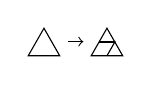
\begin{tikzpicture}[baseline]
            \draw (0, 0) -- (0.4, 0) -- (0.2, 0.35) -- cycle;
            \draw[->, thin] (0.5, 0.18) -- (0.7, 0.18);
            \draw (0.8, 0) -- (1.2, 0) -- (1.0, 0.35) -- cycle;
            \draw (0.9, 0.175) -- (1.1, 0.175) -- (1.0, 0);
            \draw (0.9, 0.175) -- (1.1, 0.175);
        \end{tikzpicture}
    };

    \node[stage, right=of s2] (s3) {%
        \textbf{3}\\[-2pt]
        \scriptsize $\Phi$ lösen\\[2pt]
        \begin{tikzpicture}[baseline]
            \shade[bottom color=viridisLow, top color=viridisHigh,
                   middle color=viridisMid]
                (0, 0) rectangle (0.6, 0.4);
            \draw (0, 0) rectangle (0.6, 0.4);
        \end{tikzpicture}
    };

    \node[stage, right=of s3] (s4) {%
        \textbf{4}\\[-2pt]
        \scriptsize Iso-Extraktion\\[2pt]
        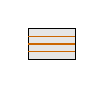
\begin{tikzpicture}[baseline]
            \fill[gray!20] (0, 0) rectangle (0.6, 0.4);
            \draw (0, 0) rectangle (0.6, 0.4);
            \draw[orange!80!black, thin] (0, 0.1) -- (0.6, 0.1);
            \draw[orange!80!black, thin] (0, 0.2) -- (0.6, 0.2);
            \draw[orange!80!black, thin] (0, 0.3) -- (0.6, 0.3);
        \end{tikzpicture}
    };

    % =========================================================
    % Reihe 2: Stufen 5 bis 8
    % =========================================================
    \node[stage, below=1.6cm of s1] (s5) {%
        \textbf{5}\\[-2pt]
        \scriptsize Branch-Tracking\\[2pt]
        
\begin{tikzpicture}[baseline]
            \draw[blue!70!black, thick] (0.3, 0) -- (0.3, 0.2);
            \draw[orange!85!black, thick] (0.3, 0.2) -- (0.1, 0.4);
            \draw[green!50!black, thick] (0.3, 0.2) -- (0.5, 0.4);
        \end{tikzpicture}
    };

    \node[stage, right=of s5] (s6) {%
        \textbf{6}\\[-2pt]
        \scriptsize Infill-Generierung\\[2pt]
        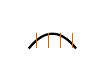
\begin{tikzpicture}[baseline]
            \draw[thick] (0, 0.05) .. controls (0.2, 0.3) and (0.4, 0.3) .. (0.6, 0.05);
            \foreach \x in {0.1, 0.25, 0.4, 0.55} {
                \draw[orange!80!black, very thin]
                    (\x, 0.05) -- (\x, 0.25);
            }
        \end{tikzpicture}
    };

    \node[stage, right=of s6] (s7) {%
        \textbf{7}\\[-2pt]
        \scriptsize Branch-Scheduling\\[2pt]
        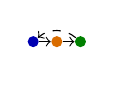
\begin{tikzpicture}[baseline]
            \node[circle, fill=blue!70!black, inner sep=0pt, minimum size=4pt] (a) at (0, 0.2) {};
            \node[circle, fill=orange!85!black, inner sep=0pt, minimum size=4pt] (b) at (0.3, 0.2) {};
            \node[circle, fill=green!50!black, inner sep=0pt, minimum size=4pt] (c) at (0.6, 0.2) {};
            \draw[->, thin] (a) -- (b);
            \draw[->, thin] (b) -- (c);
            \draw[->, thin, dashed] (c) to[bend right=40] (a);
        \end{tikzpicture}
    };

    \node[stage, right=of s7] (s8) {%
        \textbf{8}\\[-2pt]
        \scriptsize \gls{toolpath}-Konstruktion\\[2pt]
        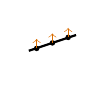
\begin{tikzpicture}[baseline]
            \draw[thick] (0, 0.1) -- (0.6, 0.3);
            \foreach \x/\y in {0.1/0.13, 0.3/0.20, 0.5/0.27} {
                \fill[black] (\x, \y) circle (1pt);
                \draw[->, very thin, orange!85!black]
                    (\x, \y) -- ++(0, 0.12);
            }
        \end{tikzpicture}
    };

    % =========================================================
    % Pfeile (ohne Labels darauf)
    % =========================================================
    \draw[flow] (s1) -- (s2);
    \draw[flow] (s2) -- (s3);
    \draw[flow] (s3) -- (s4);

    \draw[flow] (s5) -- (s6);
    \draw[flow] (s6) -- (s7);
    \draw[flow] (s7) -- (s8);

    % =========================================================
    % Umbruch-Pfeil von s4 zu s5 (explizite Koordinaten)
    % =========================================================
    \coordinate (w1) at ([xshift=0.4cm]s4.east);
    \coordinate (w2) at ([yshift=-1.05cm]w1);
    \coordinate (w3) at (w2 -| s5);
    \draw[flow] (s4.east) -- (w1) -- (w2) -- (w3) -- (s5.north);

    % =========================================================
    % Labels OBERHALB der Boxen (Reihe 1) und der Boxen (Reihe 2)
    % =========================================================
    % Reihe 1
    \node[flowlabel, anchor=south]
        at ([yshift=2pt]$(s1.north east)!0.5!(s2.north west)$)
        {\gls{mesh}};
    \node[flowlabel, anchor=south]
        at ([yshift=2pt]$(s2.north east)!0.5!(s3.north west)$)
        {verfeinertes \gls{mesh}};
    \node[flowlabel, anchor=south]
        at ([yshift=2pt]$(s3.north east)!0.5!(s4.north west)$)
        {$\Phi$, $\nabla\Phi$};

    % Wrap-Label im Zwischenraum
    \node[flowlabel]
        at ($(w2)!0.5!(w3)$)
        {Iso-Schichten};

    % Reihe 2
    \node[flowlabel, anchor=south]
        at ([yshift=2pt]$(s5.north east)!0.5!(s6.north west)$)
        {+ Branch-IDs};
    \node[flowlabel, anchor=south]
        at ([yshift=2pt]$(s6.north east)!0.5!(s7.north west)$)
        {+ \gls{infill}};
    \node[flowlabel, anchor=south]
        at ([yshift=2pt]$(s7.north east)!0.5!(s8.north west)$)
        {Druckreihenfolge};

    % =========================================================
    % Eingabe und Ausgabe
    % =========================================================
    \draw[flow] ([xshift=-0.7cm]s1.west) -- (s1.west);
    \node[iolabel, anchor=east] at ([xshift=-0.75cm]s1.west)
        {\gls{mesh}};

    \draw[flow] (s8.east) -- ([xshift=0.7cm]s8.east);
    \node[iolabel, anchor=west] at ([xshift=0.75cm]s8.east)
        {\gls{toolpath}};

\end{tikzpicture}
                    }
                    \caption[Pipeline des Kristall-Algorithmus mit acht zustandslosen Stufen.]{%
                        Verarbeitungspipeline des Kristall-Algorithmus.
                        Stufen $1$--$4$ erzeugen das Skalarfeld $\Phi$ und die Iso-Schichten; Stufen $5$--$8$ ergänzen Branch-Bezeichner, \gls{infill}, Druckreihenfolge und 6-\ac{DOF}-Posen.%
                    }
                    \label{fig:concept-crystal-pipeline}
                \end{figure}

                Im Unterschied zum Base-Algorithmus ist die Pipeline nicht queue-getrieben.
                Die Topologie des Bauteils wird nicht durch dynamisches Spawnen neuer \glspl{run}, sondern \emph{einmalig} durch die Lösung der Laplace-Gleichung erschlossen.
                Verzweigungen treten daher nicht als Steuerflussereignisse, sondern als topologische Eigenschaften der \glspl{iso-surface} in Erscheinung und werden in einer eigenen Stufe (Branch-Tracking) nachträglich identifiziert.
                \sig{Adrian Gabriel Axtmann}

            \subsubsection{Planare Basisschichten}\label{subsubsec:concept-crystal-planar-base}
                Die ersten $N_\text{base}$ Schichten werden bewusst als horizontale Ebenen geschnitten und durch Delegation an den planaren Algorithmus aus \cref{subsec:concept-planar-algorithm} erzeugt.
                Diese Entscheidung hat einen praktischen Grund: Eine gekrümmte erste Schicht hätte auf der ebenen \gls{buildplate} nur punktuellen Kontakt und würde zuverlässige Anhaftung verhindern.
                Erst oberhalb der Basisschichten setzt das nichtplanare Verfahren ein, sodass die kritische erste Bauteil-zu-Plattform-Verbindung mit dem etablierten planaren Vorgehen erfolgt.
                Die Berechnung des Skalarfeldes $\Phi$ erfolgt auf der gesamten Bauteilgeometrie einschließlich der Basisregion.
                Lediglich die Iso-Extraktion (\cref{subsubsec:concept-crystal-iso-extraction}) wird auf den Bereich $\Phi > \varphi_\text{base}$ beschränkt, wobei $\varphi_\text{base}$ dem Feldwert auf Höhe der obersten planaren Schicht entspricht.

                Die Anzahl der Basisschichten $N_\text{base}$ ist parametrierbar (Standardwert vier).
                Sie hängt vom Material und vom Bauteilformat ab.
                Stärker schwindende Materialien benötigen mehr planare Schichten, um Verzug zu vermeiden, während für leichte Bauteile eine geringere Anzahl ausreicht.
                Alle Basisschichten erhalten den \gls{branch}-Bezeichner $b = 0$ in Übereinstimmung mit der in \cref{subsubsec:concept-base-core-idea} eingeführten Konvention und eine konstante \gls{tool-orientation} entlang der \gls{build-axis}.
                Nachgelagerte Stufen unterscheiden Basis- von Iso-Schichten anhand von zwei redundanten Kriterien: dem \texttt{branch\_id}-Wert~$0$ sowie dem Schicht-Index, der unterhalb des ersten Iso-Schicht-Index liegt.
                \sig{Adrian Gabriel Axtmann}

            \subsubsection{Mesh-Verfeinerung als Voraussetzung des Solvers}\label{subsubsec:concept-crystal-mesh-refinement} \index{Mesh!Verfeinerung}
                Die Lösung der Laplace-Gleichung auf einem Dreiecksgitter ist nur dann nicht-trivial, wenn das \gls{mesh} hinreichend viele freie \glspl{vertex} zwischen den Randbedingungen besitzt.
                Auf groben Eingabe-\glspl{mesh} -- wie etwa einem CAD-Primitiv mit nur wenigen Eckvertizes -- reduziert sich das gelöste Feld auf eine lineare Rampe entlang der \gls{build-axis}.
                In diesem Fall fielen die \glspl{iso-surface} mit horizontalen Ebenen zusammen und der \emph{Kristall}-Algorithmus lieferte dieselben Schichten wie der planare Algorithmus, wenn auch unter erheblich höherem Rechenaufwand.

                Das Eingabe-\gls{mesh} wird daher vor der Feldberechnung verfeinert, bis seine längste vorhandene \gls{edge} eine parametrierbare Schwelle unterschreitet (Standardwert $1\,\text{mm}$, motiviert durch die typische Größenordnung von FDM-Düsendurchmessern).
                Besitzt das \gls{mesh} trotz erfüllter Kantenlängenbedingung weniger als 200~\glspl{vertex}, wird mindestens eine Unterteilungsrunde erzwungen.
                Dieser Fall tritt bei übermäßig dezimierter Eingabe auf, bei der zwar alle Kanten kurz sind, der Solver aber mangels Freiheitsgraden dennoch degenerieren würde.
                \glspl{mesh}, deren maximale Kantenlänge die Schwelle bereits unterschreitet und die ausreichend viele \glspl{vertex} aufweisen (z.\,B.\ Laserscan-basierte Eingaben), bleiben unverändert.

                Verwendet wird eine \emph{geometrieerhaltende} Mittelpunkt-Unterteilung.
                Jede \gls{edge} wird in der Mitte gespalten, jedes \gls{triangle} in vier Untertriangel zerlegt, und die ursprünglichen \gls{vertex}-Positionen bleiben unverändert.
                Diese Eigenschaft ist wichtig, da eine glättende Unterteilung, wie Loop-Subdivision, die Bauteilgeometrie verändern und damit die Eingangsspezifikation verletzen würde.

                Die Verfeinerung wirkt ausschließlich auf eine \emph{interne Arbeitskopie} des \glspl{mesh}.
                Das ursprüngliche \gls{mesh} bleibt für die Visualisierung und für nachfolgende Validierungsschritte unverändert verfügbar.
                Nachgelagerte Stufen der Pipeline operieren konsistent auf der verfeinerten Kopie, sodass \glspl{vertex}-Indizes und Feldwerte derselben Geometrie zuzuordnen bleiben.
                \sig{Adrian Gabriel Axtmann}

            \subsubsection{Harmonisches Skalarfeld als zentrale Datenstruktur}\label{subsubsec:concept-crystal-harmonic-field} \index{Skalarfeld!Harmonisch}\index{Laplace-Operator}
                Auf der verfeinerten Arbeitskopie wird $\Phi$ als Lösung des Randwertproblems
                \begin{equation}
                    \Delta \Phi = 0 \quad \text{im Inneren},
                    \qquad
                    \Phi|_{\Gamma_\text{unten}} = 0,
                    \qquad
                    \Phi|_{\Gamma_\text{oben}} = 1
                    \label{eq:concept-crystal-laplace}
                \end{equation}
                berechnet.

                Dabei bezeichnen $\Gamma_\text{unten}$ und $\Gamma_\text{oben}$ die der \gls{buildplate} zugewandten bzw. von ihr abgewandten Randvertizes des Bauteils, auf denen $\Phi$ jeweils fest vorgegeben wird.
                In der vorliegenden Konzeption werden beide Randmengen als zwei schmale Bänder am unteren und oberen Ende des Bauteils entlang der \gls{build-axis} festgelegt (Bandbreite je $2\,\%$ der Bauteilhöhe).
                Die Schreibweise $\Phi|_{\Gamma}$ bezeichnet hierbei die Einschränkung der Funktion $\Phi$ auf die Vertexmenge $\Gamma$, d.\,h. die Festlegung der Funktionswerte ausschließlich auf den dort liegenden Knoten.

                Da ein Computer die kontinuierliche Gleichung $\Delta\Phi = 0$ nicht direkt lösen kann, wird sie auf einem Dreiecksgitter durch ihr diskretes Analogon
                \begin{equation}
                    L\,\boldsymbol{\varphi} = 0
                    \quad\text{mit Randwerten}\quad
                    \varphi_i = \begin{cases} 0 & i \in \Gamma_\text{unten}\\ 1 & i \in \Gamma_\text{oben}\end{cases}
                    \label{eq:concept-crystal-discrete-laplace}
                \end{equation}
                ersetzt.

                Sei $V$ die Menge aller \glspl{vertex} des verfeinerten \glspl{mesh} und $\lvert V\rvert$ deren Anzahl.
                Der Vektor $\boldsymbol{\varphi} \in \mathbb{R}^{\lvert V\rvert}$ ist die diskrete Entsprechung des Skalarfeldes $\Phi$.
                Seine $i$-te Komponente $\varphi_i$ enthält den am Vertex $i$ angenommenen Feldwert.
                Während $\Phi$ also auf der gesamten Bauteilgeometrie definiert ist, ist $\boldsymbol{\varphi}$ nur an den endlich vielen Vertizes festgelegt.
                Werte dazwischen werden über die Dreiecksflächen linear interpoliert.
                Die Matrix $L \in \mathbb{R}^{\lvert V\rvert \times \lvert V\rvert}$ ist der \gls{cotangent-laplacian} und wirkt als diskreter Laplace-Operator auf den Knotenvektor.
                Anwendung von $L$ auf $\boldsymbol{\varphi}$ ergibt pro Vertex einen gewichteten Mittelwert der Differenzen zu seinen Nachbarn.
                Ist dieser Mittelwert überall null, so erfüllt $\boldsymbol{\varphi}$ die diskrete Mittelwerteigenschaft harmonischer Funktionen.

                Die Einträge von $L$ werden über die Geometrie der angrenzenden \glspl{triangle} bestimmt:
                \begin{equation}
                    L_{ij} = -\tfrac{1}{2}\bigl(\cot \alpha_{ij} + \cot \beta_{ij}\bigr),
                    \qquad
                    L_{ii} = -\sum_{j \neq i} L_{ij}
                    \label{eq:concept-crystal-cotangent}
                \end{equation}

                Hierbei bezeichnen $L_{ij}$ mit $i \neq j$ den Eintrag von $L$ in Zeile $i$ und Spalte $j$ und kodieren die Kopplung zwischen den Vertizes $i$ und $j$.
                Ein Eintrag ist nur dann von null verschieden, wenn die beiden Vertizes durch eine gemeinsame \gls{edge} verbunden sind, sodass $L$ dieselbe Sparsity-Struktur wie die Adjazenzmatrix des \glspl{mesh} besitzt.
                Die zugehörigen Gewichte ergeben sich aus den beiden Winkeln $\alpha_{ij}$ und $\beta_{ij}$, die der gemeinsamen \gls{edge} $(i, j)$ in den beiden angrenzenden \glspl{triangle} jeweils gegenüberliegen.
                Geometrisch bedeutet dies, dass an einer Kante mit annähernd rechtwinkliger Gegenüberlage die beiden Vertizes nur schwach gekoppelt werden.
                An einer Kante mit sehr spitzem Gegenwinkel hingegen entsteht eine starke Kopplung, da die beiden Vertizes dort geometrisch nahe beieinander liegen.
                Die Diagonaleinträge $L_{ii}$ werden so gewählt, dass jede Zeile zu null summiert, was die Konstanzeigenschaft harmonischer Felder ($\Delta\,\text{const} = 0$) auch im diskreten Fall garantiert \autocite[vgl.]{wardetzkyDiscreteLaplaceOperators2007}. \index{Kotangens-Gewichte}

                Die Wahl gerade dieses Operators ist durch seine mathematischen Eigenschaften begründet.
                Der \gls{cotangent-laplacian} ist symmetrisch, dünnbesetzt mit $\mathcal{O}(\lvert V\rvert)$ Nicht-Null-Einträgen und konvergiert für quasi-uniforme Gitter gegen den kontinuierlichen Laplace-Beltrami-Operator.
                Das resultierende Feld erbt drei Eigenschaften, die im Rahmen dieser Arbeit unmittelbar genutzt werden \index{Maximumprinzip}:
                \begin{description}
                    \item[Maximumprinzip] $\Phi$ besitzt im Inneren keine Extrema. Alle \glspl{iso-surface} $\Phi = \varphi^*$ mit $\varphi^* \in (0, 1)$ sind damit topologisch wohldefiniert und schließen keine inneren Hohlräume ein.
                    \item[Glattheit] $\Phi$ ist im stetigen Grenzfall $C^\infty$-glatt. Dadurch variieren $\nabla\Phi$ und somit die \gls{tool-orientation} entlang des Pfades stetig, was abrupte Drehbewegungen des Robotergelenks vermeidet.
                    \item[Geometrische Natürlichkeit] $\nabla\Phi$ steht überall senkrecht auf den \glspl{iso-surface}. Schichten und lokale Wachstumsrichtung sind damit per Konstruktion orthogonal, eine Eigenschaft, die in den ebenen Verfahren explizit erzwungen werden muss.
                \end{description}

                \cref{fig:concept-crystal-phi-field} zeigt das Skalarfeld $\Phi$ und seine Iso-Linien beispielhaft an einem T-Träger.

                \begin{figure}[ht]
                    \centering
                    \begin{tikzpicture}[
    >=Latex,
    scale=1.4,
    every node/.style={font=\small},
]
    % =========================================================
    % T-Trager mit vertikalem viridis-aehnlichem Gradient
    % Stamm: x in [-0.3, 0.3], y in [0, 2.5]
    % Querbalken: x in [-2, 2], y in [2.5, 3.0]
    % =========================================================
    \begin{scope}
        \clip
            (-0.3, 0) -- (0.3, 0) -- (0.3, 2.5) --
            (2, 2.5) -- (2, 3.0) --
            (-2, 3.0) -- (-2, 2.5) --
            (-0.3, 2.5) -- cycle;
        \shade[bottom color=viridisLow, top color=viridisHigh,
            middle color=viridisMid]
            (-2.1, -0.05) rectangle (2.1, 3.05);
    \end{scope}

    % --- T-Trager Aussenkontur ---
    \draw[thick, black]
        (-0.3, 0) -- (0.3, 0) -- (0.3, 2.5) --
        (2, 2.5) -- (2, 3.0) --
        (-2, 3.0) -- (-2, 2.5) --
        (-0.3, 2.5) -- cycle;

    % =========================================================
    % Iso-Linien (Phi = const)
    % =========================================================
    % Im Stamm: drei horizontale Linien (Phi = 0.2, 0.4, 0.6)
    \draw[white, very thick] (-0.3, 0.6) -- (0.3, 0.6);
    \node[white, font=\scriptsize, anchor=west] at (0.4, 0.6)
        {$\Phi=0{,}2$};

    \draw[white, very thick] (-0.3, 1.2) -- (0.3, 1.2);
    \node[white, font=\scriptsize, anchor=west] at (0.4, 1.2)
        {$\Phi=0{,}4$};

    \draw[white, very thick] (-0.3, 1.8) -- (0.3, 1.8);
    \node[white, font=\scriptsize, anchor=west] at (0.4, 1.8)
        {$\Phi=0{,}6$};

    % Im Querbalken: gebogene Iso-Linie (Phi = 0.85), zeigt das
    % Aufweiten in die Querbalkenarme
    \draw[white, very thick]
        (-1.8, 2.55) .. controls (-0.6, 2.95) and (0.6, 2.95) .. (1.8, 2.55);
    \node[white, font=\scriptsize, anchor=north east] at (1.85, 2.55)
        {$\Phi=0{,}85$};

    % =========================================================
    % Gradient-Pfeile (+nabla Phi, zeigt nach hoher Phi = oben)
    % =========================================================
    \foreach \x/\y in {0/0.9, 0/2.1, 1.4/2.75, -1.4/2.75} {
        \draw[->, very thick, white] (\x, \y) -- (\x, \y+0.25);
    }
    \node[white, font=\scriptsize, anchor=west] at (0.05, 0.95)
        {$+\nabla\Phi$};

    % =========================================================
    % Randbeschriftungen
    % =========================================================
    \draw[<-, thin] (0, -0.05) -- (0, -0.5);
    \node[anchor=north, font=\scriptsize, align=center] at (0, -0.5)
        {$\Gamma_\text{unten}$\\$\Phi = 0$};

    \draw[<-, thin] (0, 3.05) -- (0, 3.5);
    \node[anchor=south, font=\scriptsize, align=center] at (0, 3.5)
        {$\Gamma_\text{oben}$\\$\Phi = 1$};

    % =========================================================
    % Farbskala (rechts neben dem Bauteil)
    % =========================================================
    \begin{scope}[xshift=3.4cm]
        \shade[bottom color=viridisLow, top color=viridisHigh,
            middle color=viridisMid]
            (0, 0) rectangle (0.3, 3.0);
        \draw[thick] (0, 0) rectangle (0.3, 3.0);

        \foreach \v/\l in {0/0, 0.75/0{,}25, 1.5/0{,}5,
                        2.25/0{,}75, 3.0/1} {
            \draw (0.3, \v) -- (0.4, \v);
            \node[font=\scriptsize, anchor=west] at (0.45, \v) {\l};
        }
        \node[font=\scriptsize, anchor=south] at (0.15, 3.05) {$\Phi$};
    \end{scope}

\end{tikzpicture}
                    \caption[Skalarfeld $\Phi$ und Iso-Linien am T-Träger]{
                        Harmonisches Skalarfeld $\Phi$ auf einem T-Träger im Querschnitt (Viridis-Palette: Violett bei $\Phi=0$, Gelb bei $\Phi=1$).
                        Die Iso-Linien folgen der Bauteilgeometrie; die Gradientenpfeile $+\nabla\Phi$ geben die Werkzeugorientierung nach \cref{eq:concept-crystal-tool-frame} an.
                    }
                    \label{fig:concept-crystal-phi-field}
                \end{figure}

                Konkurrierende Felddefinitionen wurden im Vorfeld abgewogen und verworfen.
                Geodätische Distanzen lassen sich zwar mit ähnlicher Aussagekraft definieren, sind jedoch an Verzweigungspunkten nicht differenzierbar und erfordern mehrere Dijkstra-Durchläufe.
                Die \gls{heat-method} \autocite[vgl.][S.~3--4]{craneGeodesicsHeatNew2013} liefert glattere Felder, hängt aber von einem ad-hoc gewählten Diffusionszeitparameter ab.
                Der harmonische Ansatz vereint beide Vorteile, Glattheit und Parameterfreiheit und ist als linearer dünnbesetzter Solve effizient lösbar.

                Aus dem Knotenfeld $\boldsymbol{\varphi}$ wird abschließend pro \gls{triangle} der Gradient $\nabla\Phi_f$ über den diskreten Gradientenoperator $G \in \mathbb{R}^{3|F| \times |V|}$ als $\nabla\Phi_f = G_f\,\boldsymbol{\varphi}$ berechnet.
                Der so erhaltene face-weise Gradient liefert sowohl die lokale \gls{growth-direction} ($-\nabla\Phi_f$) als auch die später benötigte \gls{tool-orientation} ($+\nabla\Phi_f$).
                \sig{Adrian Gabriel Axtmann}

            \subsubsection{Adaptive Extraktion der Iso-Schichten}\label{subsubsec:concept-crystal-iso-extraction} \index{Schnittoperation!Dreieck-Iso-Fläche}
                Die Iso-Schichten werden durch Schneiden des verfeinerten \glspl{mesh} mit den Niveauflächen $\Phi = \varphi^*$ einer geordneten Folge $\varphi^*_0 < \varphi^*_1 < \dots < \varphi^*_{N-1}$ erzeugt.
                Die Wahl dieser Folge bestimmt die \emph{physikalische} Schichtdicke und ist nicht trivial, da das Verhältnis von $\Phi$-Differenz zu räumlicher Distanz spatial variiert:
                \begin{equation}
                    \Delta h_\text{phys} \;\approx\; \frac{\Delta \varphi}{|\nabla\Phi|}.
                    \label{eq:concept-crystal-physical-thickness}
                \end{equation}

                Eine uniforme $\Phi$-Schrittweite $\Delta\varphi = \text{const}$ würde in Bereichen, in denen $|\nabla\Phi|$ klein ist (z.\,B. in flachen Bauteilbereichen), zu sehr dünnen physischen Schichten führen und dort, wo $|\nabla\Phi|$ groß ist (z.\,B. in Engstellen oder an Sätteln), zu unverhältnismäßig dicken Schichten.
                Die Schrittweite wird daher \emph{adaptiv} an das lokale Gradientenfeld gekoppelt,
                \begin{equation}
                    \Delta\varphi_i \;=\; \operatorname{clamp}\bigl(t \cdot |\nabla\Phi|_\text{lokal},\; \Delta\varphi_\text{min},\; \Delta\varphi_\text{max}\bigr),
                    \label{eq:concept-crystal-adaptive-step}
                \end{equation}
                wobei $t$ die parametrierte Ziel-Schichtdicke und $|\nabla\Phi|_\text{lokal}$ der mittlere Gradientenbetrag der zuletzt extrahierten Iso-Schicht ist.
                Die untere Schranke $\Delta\varphi_\text{min}$ verhindert ein Stehenbleiben des Verfahrens in der Nähe von Sattelpunkten, an denen $|\nabla\Phi| \to 0$ gilt.
                Die obere Schranke $\Delta\varphi_\text{max}$ verhindert das Überspringen ganzer Bauteilregionen an Engstellen, an denen $|\nabla\Phi|$ sehr groß werden kann.
                Beide Schranken werden als Vielfache der uniformen Referenzschrittweite $\Delta\varphi_\text{uniform} = t/h_\text{mesh}$ bestimmt und sind damit dimensions- und bauteilskalenfrei.

                Die Schnittoperation pro $\varphi^*$ beruht auf derselben Grundidee wie der Ebene-Dreieck-Schnitt aus \cref{subsubsec:concept-planar-plane-intersection}, ersetzt aber die signierte Distanz zur \gls{slice-plane} durch die Differenz $d_j = \varphi_j - \varphi^*$ am \gls{vertex} $j$.
                Eine \gls{edge} zwischen $\vec{v}_A$ und $\vec{v}_B$ schneidet die \gls{iso-surface} genau dann, wenn $\operatorname{sgn}(d_A) \neq \operatorname{sgn}(d_B)$ und der Schnittpunkt ergibt und sich linear interpoliert zu $\vec{P} = \vec{v}_A + \tau (\vec{v}_B - \vec{v}_A)$ mit $\tau = d_A / (d_A - d_B)$.
                Die in \cref{subsubsec:concept-planar-plane-intersection} diskutierten Sonderfälle (\gls{vertex}, \gls{edge} oder \gls{triangle} exakt auf der Iso-Fläche) gelten unverändert.
                Ihnen wird zusätzlich dadurch vorgebeugt, dass der Niveauwert $\varphi^*$ geringfügig verschoben wird, sobald ein \gls{vertex} näher als $10^{-5} \cdot (\varphi_{\max} - \varphi_{\min})$ an die Iso-Fläche kommt.
                Die Verschiebung selbst beträgt $10^{-4} \cdot (\varphi_{\max} - \varphi_{\min})$.

                Die so gewonnenen \glspl{line-segment} werden pro \gls{iso-step} und pro zusammenhängender Komponente getrennt mit dem aus \cref{subsubsec:concept-planar-contour-chaining} bekannten gierigen \gls{nearest-neighbor} zu \glspl{contour-ring} verkettet.
                Pro Endpunkt wird zusätzlich der pro-\gls{triangle} berechnete Gradient $+\nabla\Phi$ als \gls{tool-orientation} mitgeführt.
                Die Verkettungsstufe muss diese Information lediglich entlang der Punktreihenfolge mit transportieren.

                Da ein Iso-Schnitt durch einen Mesh-Vertex die Verkettung in mehrere benachbarte Teilringe fragmentieren kann, werden nach der Verkettung Ringe, deren Schwerpunkte näher als eine parametrierte Verschmelzungs\-distanz liegen oder deren Bounding Boxes sich überlappen, durch ein greedy Union-Find zu einer einzigen zusammenhängenden Komponente zusammengeführt.
                Dies entspricht einer numerischen Robustheitsmassnahme und verändert die topologische Struktur des Ergebnisses bei geometrisch klar getrennten Komponenten nicht.
                \sig{Adrian Gabriel Axtmann}

            \subsubsection{Branch-Tracking auf Iso-Schichten}\label{subsubsec:concept-crystal-branch-tracking} \index{Zweig!Tracking}
                Eine einzelne Iso-Schicht $\Phi = \varphi^*_i$ kann, abhängig von der Topologie des Bauteils, in mehrere räumlich getrennte Komponenten zerfallen.
                Bei einem T-förmigen Bauteil z.\,B. ist die Iso-Fläche im unteren Stegbereich einfach zusammenhängend, im oberen Querbalken jedoch in zwei Komponenten gespalten, je eine pro Querbalkenarm.
                Damit nachfolgende Stufen, insbesondere das Branch-Scheduling, benachbarte Komponenten als zusammengehörig erkennen können, muss jeder Komponente ein über mehrere \glspl{iso-step} \emph{stabiler} \gls{branch}-Bezeichner zugewiesen werden.

                Das Verfahren wird als gierige Zuordnung über Schwerpunkte aufeinanderfolgender \glspl{iso-step} formuliert.
                Pro Komponente wird der Schwerpunkt $\vec{c}_k$ ihrer Konturpunkte berechnet.
                Im ersten \gls{iso-step} oberhalb der planaren Basis erhält jede Komponente einen frischen Bezeichner.
                In jedem darauf folgenden \gls{iso-step} wird jeder neuen Komponente $d$ derjenige Vorgänger $a$ aus dem unmittelbar vorangegangenen \gls{iso-step} zugeordnet, für den $\lVert\vec{c}_d - \vec{c}_a\rVert$ minimal ist und unterhalb einer \gls{drift-threshold} liegt.

                Die \gls{drift-threshold} ist als
                \begin{equation}
                    \delta_\text{drift} \;=\; \max\!\bigl(\delta_\text{min},\; k_\text{drift} \cdot t\bigr)
                    \label{eq:concept-crystal-drift-threshold}
                \end{equation}
                definiert, wobei $\delta_\text{min}$ ein konstantes Minimum (Standardwert $0{,}5\,\text{mm}$) und $k_\text{drift}$ ein Vielfaches der \gls{layer-height} (Standardwert $4$) bezeichnet.
                Die Schranke kodiert die geometrische Annahme, dass eine zusammenhängende Komponente zwischen zwei \glspl{iso-step}[n] maximal um wenige Schichtdicken wandern kann.
                Größere Sprünge werden als topologisches Ereignis interpretiert.

                Aus der Zuordnung lassen sich vier Topologie-Ereignisse ableiten, die für die spätere Analyse und Visualisierung des \glspl{slicing} dokumentiert werden:

                \begin{description}
                    \item[Birth] Eine neue Komponente besitzt keinen Vorgänger innerhalb von $\delta_\text{drift}$ und erhält einen frischen Bezeichner.
                    \item[Death] Ein Vorgänger besitzt keinen Nachfolger. Der zugehörige \gls{branch} terminiert (Spitze erreicht).
                    \item[Split] Ein Vorgänger wird mehreren Nachfolgern zugeordnet. Alle bis auf den nächstgelegenen erhalten frische Bezeichner. Dieses Ereignis tritt typischerweise an Verzweigungen auf (T-Querbalken zerfällt in zwei Arme).
                    \item[Merge] Mehrere Vorgänger werden demselben Nachfolger zugeordnet. Das tritt bei monotonem $\Phi$ nur in Ausnahmefällen auf (Schließen einer Bohrung).
                \end{description}

                \cref{fig:concept-crystal-branch-tracking} illustriert das Branch-Tracking am Beispiel des T-Trägers.

                \begin{figure}[ht]
                    \centering
                    \begin{tikzpicture}[
    >=Latex,
    every node/.style={font=\small},
]
    % =========================================================
    % (a) Persistence-aehnliches Diagramm
    % =========================================================
    \node[font=\bfseries, anchor=west] at (0, 3.0)
        {(a) Topologie-Evolution über die Iso-Stufen};

    % Achsen
    \draw[->, thick] (-0.3, 0) -- (10, 0)
        node[anchor=west, font=\scriptsize] {$\varphi^*$};

    % X-Skala
    \foreach \x/\v in {0/0, 2.5/0{,}25, 5/0{,}5, 7.5/0{,}75, 10/1} {
        \draw (\x, -0.1) -- (\x, 0.1);
        \node[anchor=north, font=\scriptsize] at (\x, -0.15) {\v};
    }

    % Iso-Stufen (gestrichelte Hilfslinien)
    \foreach \x in {1, 2, 3, 4, 5, 6, 7, 8, 9} {
        \draw[gray!40, dotted, very thin] (\x, -1.8) -- (\x, 2.5);
    }

    % --- LINIEN (zuerst zeichnen, damit Symbole obenauf liegen) ---
    % Stamm-Branch (b=0) von phi*=0 bis exakt phi*=0.5 (x=5)
    \draw[ultra thick, blue!70!black] (0.3, 0) -- (5.0, 0);
    
    % Zweig 1 (b=1, oben) nach Split
    \draw[ultra thick, orange!85!black] (5.0, 0) -- (5.5, 1.5) -- (10, 1.5);
    
    % Zweig 2 (b=2, unten) nach Split
    \draw[ultra thick, green!50!black] (5.0, 0) -- (5.5, -1.5) -- (10, -1.5);


    % --- SYMBOLE & TEXTE (liegen nun sauber über den Linien) ---
    % Stamm Text
    \node[font=\scriptsize, blue!70!black, anchor=south, align=center]
        at (2.5, 0.15) {Stamm $b=0$};

    % Zweig Texte
    \node[font=\scriptsize, orange!85!black, anchor=south]
        at (8, 1.65) {Zweig $b=1$};
    \node[font=\scriptsize, green!50!black, anchor=north]
        at (8, -1.65) {Zweig $b=2$};

    % Birth-Symbol (offener Kreis) am Stammbeginn
    \draw[blue!70!black, fill=white, thick] (0.3, 0) circle (0.13);
    \node[font=\scriptsize, anchor=south] at (0.3, 0.25) {Birth};

    \draw[red!80!black, fill=red!20, thick]
        (5.0, -0.18) -- (5.0, 0.18) -- (5.45, 0) -- cycle;
    \node[font=\scriptsize, red!80!black, anchor=south]
        at (4.5, 0.15) {Split};

    % Death-Symbole (gefuellte Kreise) am Ende
    \draw[orange!85!black, fill=orange!85!black, thick]
        (10, 1.5) circle (0.13);
    \draw[green!50!black, fill=green!50!black, thick]
        (10, -1.5) circle (0.13);
    \node[font=\scriptsize, anchor=west] at (10.2, 1.5) {Death};
    \node[font=\scriptsize, anchor=west] at (10.2, -1.5) {Death};

    % =========================================================
    % (b) T-Traeger-Referenz (klein, unten links)
    % =========================================================
    \begin{scope}[xshift=1.5cm, yshift=-4.2cm, scale=0.6]
        \node[font=\bfseries, anchor=west] at (-1.5, 2.2)
            {(b) Zugehöriges Bauteil};

        % Farbige Füllungen
        \fill[blue!30] (-0.3, -0.5) rectangle (0.3, 1.5);     % Kompletter Stamm
        \fill[green!40] (-1.5, 1.0) rectangle (-0.3, 1.5);    % Linker Querbalken (b=2)
        \fill[orange!40] (0.3, 1.0) rectangle (1.5, 1.5);     % Rechter Querbalken (b=1)

        \draw[thick] (-0.3, 1.0) -- (-0.3, 1.5);
        \draw[thick] (0.3, 1.0) -- (0.3, 1.5);

        % Äußere Umrandung
        \draw[thick]
            (-0.3, -0.5) -- (0.3, -0.5) -- (0.3, 1.0) --
            (1.5, 1.0) -- (1.5, 1.5) --
            (-1.5, 1.5) -- (-1.5, 1.0) --
            (-0.3, 1.0) -- cycle;

        % Branch-Beschriftungen
        \node[font=\tiny, blue!70!black] at (0, -1.0) {$b=0$};
        \node[font=\tiny, orange!85!black] at (0.9, 0.75) {$b=1$};
        \node[font=\tiny, green!50!black] at (-0.9, 0.75) {$b=2$};
    \end{scope}

    % =========================================================
    % (c) Legende der Topologie-Ereignisse (rechts neben Bauteil)
    % =========================================================
    \begin{scope}[xshift=6.5cm, yshift=-4.2cm]
        \node[font=\bfseries, anchor=west] at (0, 1.5)
            {(c) Topologie-Ereignisse};

        % Birth
        \draw[black, fill=white, thick] (0.2, 1.0) circle (0.10);
        \node[font=\scriptsize, anchor=west] at (0.4, 1.0)
            {Birth: neue Komponente};

        % Death
        \draw[black, fill=black, thick] (0.2, 0.6) circle (0.10);
        \node[font=\scriptsize, anchor=west] at (0.4, 0.6)
            {Death: Komponente endet};

        % Split
        \draw[red!80!black, fill=red!20, thick]
            (0.1, 0.1) -- (0.1, 0.3) -- (0.3, 0.2) -- cycle;
        \node[font=\scriptsize, anchor=west] at (0.4, 0.2)
            {Split: Aufspaltung};

        % Merge
        \draw[red!80!black, fill=red!20, thick]
            (0.3, -0.4) -- (0.3, -0.2) -- (0.1, -0.3) -- cycle;
        \node[font=\scriptsize, anchor=west] at (0.4, -0.3)
            {Merge: Zusammenführung};
    \end{scope}

\end{tikzpicture}
                    \caption[Branch-Tracking am T-Träger als Topologie-Diagramm]{
                        (a)~Evolution der zusammenhängenden Komponenten der Iso-Flächen $\Phi = \varphi^*$ über den Wertebereich von $\varphi^*$.
                            Der Stamm-Branch $b=0$ entsteht an der unteren Randregion und spaltet sich beim Erreichen des Querbalkens in zwei Zweig-Branches $b=1$ und $b=2$ auf, die jeweils an der oberen Randregion enden.
                        (b)~Das zugehörige Bauteil mit den entsprechend eingefärbten Branch-Regionen.
                        (c)~Legende der vier möglichen Topologie-Ereignisse.
                    }
                    \label{fig:concept-crystal-branch-tracking}
                \end{figure}

                Anders als beim Base-Algorithmus werden \glspl{branch} also nicht durch geometrische Überhangerkennung \emph{erzeugt}, sondern als topologische Eigenschaft des bereits berechneten Skalarfeldes \emph{nachträglich identifiziert}.
                Die Trennung zwischen Felddefinition in Stufe 3 und Topologieanalyse in Stufe 5 erlaubt es, beide Stufen unabhängig voneinander zu validieren.
                \sig{Adrian Gabriel Axtmann}

            \subsubsection{Infill-Generierung auf gekrümmten Schichten}\label{subsubsec:concept-crystal-infill} \index{Infill!Nicht-planar}
                Während die planaren Basisschichten dasselbe achsenparallele Scanline-Muster wie der planare Algorithmus verwenden, erfordert das \gls{infill} auf \emph{gekrümmten} Iso-Schichten zusätzliche Schritte.
                Ein zweidimensionales Muster lässt sich nicht direkt auf eine dreidimensional gekrümmte Fläche übertragen, ohne entweder die Liniendichte zu verzerren oder die Zugehörigkeit der Linien zur \gls{iso-surface} zu verlieren.

                Das Problem wird durch eine zweistufige Konstruktion gelöst.
                Zunächst wird in der lokalen Tangentialebene jeder Iso-Schicht ein klassisches zweidimensionales Scanline-\gls{infill} erzeugt und anschließend punktweise wieder auf die gekrümmte \gls{iso-surface} \emph{angehoben}.

                \paragraph{Tangentialebene und Hauptachsen}
                    Pro Komponente werden der Schwerpunkt $\vec{c}$ und die mittlere Normale $\hat{n} = \overline{\nabla\Phi}\,/\,\lVert\overline{\nabla\Phi}\rVert$ aus den Konturpunkten und ihren mitgeführten Gradienten berechnet.
                    Senkrecht zu $\hat{n}$ wird mittels \gls{gram-schmidt} eine vorläufige orthonormale Tangentialbasis $(\hat{u}_0, \hat{v}_0)$ aufgespannt.
                    Anschließend werden die Konturpunkte in diese Basis projiziert, und die Hauptachsen der projizierten Punktwolke werden mittels \gls{pca} bestimmt.
                    $(\hat{u}, \hat{v})$ wird so rotiert, dass $\hat{u}$ entlang der Hauptachse zeigt.
                    Diese Ausrichtung sorgt dafür, dass die Scanlinien längs der ausgedehnten Komponentenrichtung verlaufen und die Anzahl der Scanlinien pro Komponente nahezu minimal wird.
                    Bei nahezu isotroper Punktwolke (Eigenwertverhältnis $\lambda_2/\lambda_1 > 0{,}7$) ist die \gls{pca} numerisch instabil.
                    In diesem Fall wird auf eine globale Referenzrichtung (Welt-$X$, in die Tangentialebene projiziert) zurückgegriffen.
                    Zur Erzeugung von Kreuzungsmustern wird die Basis $(\hat{u}, \hat{v})$ in Abhängigkeit des maximalen Normalabstands der Konturpunkte von der Tangentialebene adaptiert.
                    Bei schwach gekrümmten (nahezu planaren) Schichten wird $(\hat{u}, \hat{v})$ jede zweite Schicht um $90^\circ$ gedreht, um ein alternierendes Schraffurmuster zu erzeugen.
                    Bei stark gekrümmten Schichten, deren Konturpunkte mehr als $0{,}5\,\text{mm}$ aus der Tangentialebene herausragen, wird die Basis fest um $90^\circ$ rotiert, sodass $\hat{u}$ auf die PCA-Nebenachse zeigt und die Scanlinien längs der Hauptausdehnung verlaufen.
                    \sig{Adrian Gabriel Axtmann}

                \paragraph{Scanline-Sweep in der Tangentialebene}
                    In der so festgelegten $(\hat{u},\hat{v})$-Ebene werden parallele Scanlinien im Abstand des parametrierten \gls{infill-spacing} aufgespannt.
                    Die Schnitte jeder Scanlinie mit dem projizierten Konturpolygon werden über die \gls{even-odd-rule} zu Linienpaaren zusammengefasst und nach der \gls{snake-pattern} alternierend orientiert, um Verbindungswege zwischen aufeinanderfolgenden Linien zu vermeiden.
                    \sig{Adrian Gabriel Axtmann}

                \paragraph{Anhebung auf die Iso-Fläche mittels IDW}
                    Die so gewonnenen Punkte liegen ausschließlich in der \emph{Tangentialebene}, nicht aber auf der gekrümmten \gls{iso-surface}.
                    Eine direkte Rückprojektion entlang $\hat{n}$ wäre möglich, würde aber bei stark gekrümmten Schichten zu fehlerhaften Schnitten mit Bauteilwänden führen.
                    Daher wird pro $(u, v)$-Punkt eine \gls{idw} über die $k$ nächsten Konturpunkte (in der $(u,v)$-Projektion) durchgeführt: \index{Inverse Distance Weighting}
                    \begin{equation}
                        \vec{p}_\text{3D}(u, v) \;=\; \frac{\sum_i w_i \cdot \vec{p}_i^{\,\text{Kontur}}}{\sum_i w_i},
                        \qquad
                        w_i \;=\; \frac{1}{\lVert(u,v) - (u_i, v_i)\rVert^2 + \varepsilon}.
                        \label{eq:concept-crystal-idw}
                    \end{equation}
                    Da die Konturpunkte $\vec{p}_i^{\,\text{Kontur}}$ per Konstruktion exakt auf $\Phi = \varphi^*$ liegen, interpoliert die Gewichtung jedes Infill-Punkt zwischen ihnen und liefert eine sehr gute Näherung an die echte \gls{iso-surface}, ohne dass eine erneute geometrische Verschneidung mit dem \gls{mesh} erforderlich wird.
                    Die Konstante $\varepsilon$ verhindert numerisch eine Division durch null in der Nähe eines Konturpunkts.
                    Da die IDW-Interpolation zwischen den bekannten Iso-Schicht-Punkten interpoliert, bleiben die Infill-Punkte typischerweise nah an der Iso-Fläche.
                    Eine explizite Abstandsvalidierung ist in der aktuellen Implementierung nicht vorhanden.

                    Die so erzeugten Infill-\glspl{line-segment} werden an die Wandkontur der Schicht angehängt.
                    Eine Markierung trennt die Indizes der Wandsegmente von denen der Infill-Segmente, sodass die nachgelagerte \gls{toolpath}-Konstruktion beide Bestandteile mit unterschiedlichen Druckparametern versehen kann.
                    \sig{Adrian Gabriel Axtmann}

            \subsubsection{Branch-Scheduling und Massebalance}\label{subsubsec:concept-crystal-branch-scheduling} \index{Zweig!Scheduling}
                Würden die Schichten in der Reihenfolge ihrer Erzeugung gedruckt, so würde zunächst der gesamte erste \gls{branch} bis zu ihrer Spitze gefertigt, bevor mit dem zweiten \gls{branch} begonnen wird.
                Bei symmetrischen Geometrien wie einem T-förmigen Bauteil führt dieses Vorgehen zu einer einseitigen Massenkonzentration und erhöht die Kippgefahr während des Drucks.
                Aus thermischer Sicht hat ein bereits vollständig fertiggestellter Arm zudem deutlich mehr Zeit zum Abkühlen als der noch zu fertigende, was zu Spannungen an der Verbindungsstelle führt.

                Die Schichtreihenfolge wird daher \emph{nach} dem Slicen, aber \emph{vor} der Konstruktion des \glspl{toolpath}, durch eine austauschbare Strategie umgeordnet.
                Hierzu werden die Schichten zunächst nach \gls{iso-step} gruppiert.
                Innerhalb jedes \gls{iso-step}[s] wird die Reihenfolge der Komponenten von einer konkreten Strategie bestimmt.
                Die Standardstrategie ist eine \emph{alternierende Round-Robin-Reihenfolge}.
                Pro \gls{iso-step} wird jeder \gls{branch} genau einmal abgearbeitet, bevor zum nächsten \gls{iso-step} übergegangen wird.
                Damit wächst das Bauteil schichtweise in allen \glspl{branch}[n] parallel, und die Massenverteilung bleibt während des gesamten Drucks symmetrisch.

                Entscheidend ist die Trennung von \emph{Schichterzeugung} und \emph{Schichtreihenfolge}.
                Die Erzeugung der Schichten ist deterministisch durch das Skalarfeld vorgegeben und unabhängig vom späteren Druckablauf.
                Die Reihenfolge ist dagegen ein freier Parameter, der sich an Material, Geometrie und Hardware anpassen lassen muss.
                Die Strategie wird daher als abstraktes Interface nach dem \gls{strategy-pattern} modelliert.
                Alternative Verfahren wie \glqq $N$ Schichten pro \gls{branch}\grqq für langsame thermische Zyklen oder eine streng symmetrische Paar-Reihenfolge für hochsymmetrische Bauteile lassen sich so ohne Änderung der übrigen Pipeline integrieren.
                \sig{Adrian Gabriel Axtmann}

            \subsubsection{Toolpath-Konstruktion und Werkzeugorientierung}\label{subsubsec:concept-crystal-tool-orientation} \index{Werkzeugorientierung!Crystal}
                Die Konstruktion des \glspl{toolpath} überführt die geordnete Schichtfolge nach dem Branch-Scheduling in eine chronologisch geordnete Folge von \glspl{segment}, die von \ac{kronos} als Roboterbewegungen ausgeführt werden.
                Jedes \gls{segment} trägt Anfangspunkt, Endpunkt und eine Werkzeugorientierung sowie vier Metadaten-Felder: den \gls{branch}-Bezeichner, den Wachstumsschritt (Schicht-Index), ein Infill-Kennzeichen und ein Verbindungsbewegungs-Kennzeichen.

                Die Werkzeugorientierung wird pro Segment als normierter Vektor $\hat{z}_\text{tool}$ aus den am Anfangs- und Endpunkt mitgeführten Gradientenwerten bestimmt,
                \begin{equation}
                    \hat{z}_\text{tool}
                    \;=\;
                    \frac{\nabla\Phi_{\vec{a}} + \nabla\Phi_{\vec{e}}}
                        {\lVert\nabla\Phi_{\vec{a}} + \nabla\Phi_{\vec{e}}\rVert},
                    \label{eq:concept-crystal-tool-frame}
                \end{equation}
                wobei $\nabla\Phi_{\vec{a}}$ und $\nabla\Phi_{\vec{e}}$ die face-weise berechneten Gradientenvektoren am Anfangs- bzw.\ Endpunkt des Segments sind (vgl.\ \cref{subsubsec:concept-crystal-harmonic-field}).
                Da $+\nabla\Phi$ per Konstruktion senkrecht auf der Iso-Fläche steht und vom Bauteil weg zeigt, entspricht $\hat{z}_\text{tool}$ der Werkzeugachse in der \ac{ROS}-2\slash{}MoveIt-Konvention.
                Degeneriert der Gradient ($\lVert\nabla\Phi_{\vec{a}} + \nabla\Phi_{\vec{e}}\rVert < 10^{-8}$), wird als Rückfallwert die \gls{build-axis} eingesetzt.

                Eine vollständige 6-\ac{DOF}-Pose — bestehend aus einem rechtshändigen orthonormalen Dreibein $(\hat{x}_\text{tool}, \hat{y}_\text{tool}, \hat{z}_\text{tool})$ mit $\hat{x}_\text{tool}$ entlang der Segmentrichtung und $\hat{y}_\text{tool} = \hat{z}_\text{tool} \times \hat{x}_\text{tool}$ sowie der daraus abgeleiteten \gls{quaternion} — ist als nächster Implementierungsschritt vorgesehen.
                In der vorliegenden Version wird ausschließlich $\hat{z}_\text{tool}$ als skalarer Orientierungsvektor pro Segment gespeichert.

                \paragraph{Erkennung von Verbindungswegen}
                    Zwei aufeinanderfolgende Segmente werden genau dann als \emph{Druckbewegung} verbunden, wenn der Endpunkt des vorhergehenden Segments innerhalb einer engen Toleranz von $1\,\mu\text{m}$ mit dem Startpunkt des nachfolgenden zusammenfällt und beide Segmente demselben \gls{branch} angehören.
                    Andernfalls wird zwischen ihnen ein nicht-extrudierender \gls{travel-move} eingefügt, dessen Orientierung von der Orientierung des nachfolgenden Drucksegments übernommen wird.
                    Diese explizite Markierung ist Voraussetzung dafür, dass \ac{kronos} Druck- und Verbindungsbewegungen mit unterschiedlichen Geschwindigkeitsprofilen versieht.
                    \sig{Adrian Gabriel Axtmann}

            \subsubsection{Voraussetzungen und Grenzen}\label{subsubsec:concept-crystal-assumptions-limits}
                Zusätzlich zu den in \cref{sec:concept-of-slicing-strategies} formulierten gemeinsamen Voraussetzungen stellt der Kristall-Algorithmus zwei weitere Anforderungen, die aus der Verwendung des harmonischen Solvers resultieren:

                \begin{description}
                    \item[Hinreichende Vertexdichte]
                        Das verfeinerte \gls{mesh} muss zwischen $\Gamma_\text{unten}$ und $\Gamma_\text{oben}$ genügend freie \glspl{vertex} besitzen, damit die Lösung der Laplace-Gleichung nicht zu einer linearen Rampe entartet.
                        Die in \cref{subsubsec:concept-crystal-mesh-refinement} beschriebene Verfeinerungsstufe stellt diese Voraussetzung automatisch her, sofern sie nicht explizit deaktiviert wird.
                    \item[Eindeutig identifizierbare Randbänder]
                        $\Gamma_\text{unten}$ und $\Gamma_\text{oben}$ werden anhand der Bauteilextrema entlang der \gls{build-axis} als schmale Bänder festgelegt.
                        Bauteile, deren \gls{buildplate}-Kontaktfläche nicht entlang der \gls{build-axis} liegt (z.\,B. gekippte Bauteile), erfüllen diese Annahme nicht und liefern verzerrte Iso-Schichten.
                \end{description}

                Folgende Grenzen werden bewusst akzeptiert:
                \begin{itemize}
                    \item \textbf{Keine echte adaptive Schichtdicke}
                        Adaptiv ist nur die $\Phi$-Schrittweite, sodass die \emph{physikalische} Schichtdicke näherungsweise konstant bleibt.
                        Eine an die lokale Krümmung der Bauteiloberfläche angepasste Schichtdicke wird nicht umgesetzt.
                    \item \textbf{Eine einzige Wandkontur pro Schicht}
                        Mehrwandige Konturen erfordern ein geodätisches Versatzverfahren auf gekrümmten Flächen, welches im Rahmen dieser Arbeit nicht implementiert wird.
                    \item \textbf{Genau eine zusammenhängende Basisregion}
                        Der Algorithmus geht von genau einer \gls{buildplate}-Kontaktregion aus.
                        Mehrteilige Bauplätze würden separate $\Phi$-Lösungen pro Teil erfordern.
                    \item \textbf{Approximative Lage der Infill-Punkte}
                        Durch die \gls{idw}-Anhebung können Infill-Punkte um bis zu einer \gls{layer-height} von der exakten \gls{iso-surface} abweichen.
                        Für die hier betrachteten Geometrien ist diese Abweichung tolerierbar.
                \end{itemize}

                Die in \cref{sec:concept-of-slicing-strategies} festgehaltene Branch-Kollisionserkennung gilt unverändert.

                \cref{tab:concept-crystal-vs-all} stellt den Kristall-Algorithmus allen zuvor beschriebenen Verfahren (planar, Base, Sphären) gegenüber.
                \sig{Adrian Gabriel Axtmann}

                \begin{table}[ht]
                    \centering
                    \scriptsize
                    \caption[Vergleich aller vier Slicing-Algorithmen]
                            {Vergleich aller vier Slicing-Algorithmen}
                    \label{tab:concept-crystal-vs-all}
                    \renewcommand{\arraystretch}{1.2}
                    \setlength{\emergencystretch}{2em}
                    \begin{tabularx}{\linewidth}{@{}
                        >{\raggedright\arraybackslash\hspace{0pt}}p{2.6cm}
                        >{\raggedright\arraybackslash\hspace{0pt}}X
                        >{\raggedright\arraybackslash\hspace{0pt}}X
                        >{\raggedright\arraybackslash\hspace{0pt}}X
                        >{\raggedright\arraybackslash\hspace{0pt}}X @{}}
                        \toprule
                        \textbf{Eigenschaft} & \textbf{Planar} & \textbf{Base} & \textbf{Sphären} & \textbf{Kristall} \\
                        \midrule
                        Schicht\-geometrie
                            & ebene \glspl{slice-plane}
                            & ebene Stücke pro \gls{run}
                            & \glspl{sphere-shell}
                            & gekrümmte \glspl{iso-surface} $\Phi = \mathrm{const}$ \\
                        \addlinespace
                        Schicht\-para\-metrierung
                            & Höhe $h$
                            & Höhe $h$ pro \gls{run}
                            & Radius $r$
                            & Iso-Wert $\varphi^{*}$ \\
                        \addlinespace
                        Schichtdicke
                            & konstant
                            & konstant pro \gls{run}
                            & konstant in $\Delta r$
                            & konstant in $h$, adaptiv in $\Delta\varphi$ \\
                        \addlinespace
                        Wachstums\-richtungen
                            & genau eine, statisch
                            & vier diskrete pro \gls{run}
                            & kontinuierlich radial
                            & kontinuierlich aus $-\nabla\Phi$ \\
                        \addlinespace
                        Topologie\-erschließung
                            & keine
                            & dynamisch per Queue
                            & dynamisch per Queue
                            & einmalig per Feldlösung mit Branch-Tracking \\
                        \addlinespace
                        \Gls{tool-orientation}
                            & konstant entlang \gls{build-axis}
                            & pro \gls{run} konstant
                            & radial, analytisch
                            & pro Segment aus $+\nabla\Phi$ \\
                        \addlinespace
                        \Gls{overhang}-Behandlung
                            & nicht vorgesehen
                            & \gls{branch}-Spawning
                            & Spawnen neuer \gls{sphere-center}
                            & implizit durch Feldgeometrie \\
                        \addlinespace
                        Kontur-Topologie
                            & geschlossene Ringe
                            & einzelne Segmentpaare
                            & geschlossene Ringe auf Schale
                            & Ringe pro zusammen\-hängender Komponente \\
                        \addlinespace
                        \Gls{infill}
                            & planar, achsen\-parallel
                            & planar, achsen\-parallel pro \gls{run}
                            & nicht spezifiziert
                            & in lokaler Tangentialebene mit \gls{idw}-Anhebung \\
                        \addlinespace
                        Rechenkosten
                            & sehr gering
                            & gering
                            & gering bis mittel
                            & dominiert durch dünnbesetzten Solver \\
                        \addlinespace
                        Anwendungs\-schwerpunkt
                            & prismatische Bauteile, Baseline
                            & lokalisierte \glspl{overhang}
                            & radial-sym\-me\-trische Bauteile
                            & flächige Krümmung, baum\-artige Topologie \\
                        \addlinespace
                        Umsetzungs\-stand
                            & implementiert
                            & implementiert
                            & nur konzeptionell
                            & implementiert \\
                        \bottomrule
                    \end{tabularx}
                \end{table}